\documentclass[a4paper]{jreport}
\newcommand{\version}{4.3.3}

\title{{\vspace{2cm}{\Large Version \version} }}
\author{\Large Team SCALE\\ UGC working group}
\date{\today}


\usepackage[dvipdfmx]{graphicx, color}
\usepackage[dvipdfmx]{hyperref}
\usepackage{amsmath}
\usepackage{ascmac}
\usepackage{alltt}
\usepackage[round]{natbib}
\usepackage{tabularx}
\usepackage{color}
\usepackage{colortbl}
\usepackage{fancybox}
\usepackage{url}
\usepackage{pxjahyper}
\hypersetup{% options for hyperref
 bookmarksopen=true,
 bookmarksnumbered=true,
 colorlinks=true,
% linkcolor=red,
 linkcolor=cyan,
 citecolor=cyan,
 urlcolor=cyan,
}

%\setlength{\textwidth}{42zw}
%\setlength{\textheight}{40\baselineskip}
\usepackage[top=30mm,bottom=35mm,left=30mm,right=30mm]{geometry}
\usepackage{wallpaper}
%\renewcommand{\thefootnote}{\fnsymbol{footnote}}
\renewcommand{\thefootnote}{*\arabic{footnote})}

\newcommand{\namelist}[1]{{\color{magenta}\texttt{[\detokenize{#1}]}}}
\newcommand{\nmitem}[1]{{\color{magenta}\texttt{(\detokenize{#1})}}}
%数式モード
\newcommand{\nmitemeq}[1]{{\texttt{\detokenize{#1}}}}
\newcommand{\XDIR}{X方向}
\newcommand{\YDIR}{Y方向}
\newcommand{\ZDIR}{Z方向}

%%%%
%%%% for chapter 5
\newcommand{\SecBasicDomainSetting}{{対象計算領域の設定}}
\newcommand{\SubsecMPIProcess}{{MPIプロセス数の設定}}
\newcommand{\SubsecGridNumSettng}{{水平・鉛直格子数の設定}}
\newcommand{\SubsecGridIntvSettng}{{水平・鉛直格子間隔の設定}}
\newcommand{\SubsecRayleighDampingSetting}{{スポンジ層の設定}}
\newcommand{\SubsecBasicBufferSetting}{{緩和領域と境界ナッジングの設定}}
\newcommand{\SecMapprojectionSetting}{{地図投影法と計算領域の位置の設定}}
\newcommand{\SecBasicTopoSetting}{{地形の設定}}
\newcommand{\SecInputDataSetting}{{初期値・境界値データの作成方法}}
\newcommand{\SecBasicIntegrationSetting}{{積分時間と時間刻み幅の設定}}
\newcommand{\SecBasicOutputSetting}{{出力変数の追加・変更方法}}
\newcommand{\SecBasicDynamicsSetting}{{力学スキーム}}
\newcommand{\SubsecDynsolverSetting}{{数値解法の設定}}
\newcommand{\SubsecDynSchemeSetting}{{時間・空間差分スキーム}}
\newcommand{\SecBasicPhysicsSetting}{{物理スキームの設定}}
\newcommand{\SubsecMicrophysicsSetting}{{雲微物理スキーム}}
\newcommand{\SubsecTurbulenceSetting}{{乱流スキーム}}
\newcommand{\SubsecRadiationSetting}{{放射スキーム}}
\newcommand{\SubsecSurfaceSetting}{{地表面(大気下端境界)の設定}}
\newcommand{\SubsecOceanSetting}{{海洋モデル}}
\newcommand{\SubsecLandSetting}{{陸面モデル}}
\newcommand{\SubsecUrbanSetting}{{都市モデル(大気-都市面フラックス)}}
\newcommand{\SecAdvancePostprosess}{{後処理}}
\newcommand{\SecAdvanceRestart}{{リスタート計算の方法}}
\newcommand{\SecAdvanceNesting}{{領域ネスティング実験の方法}}
\newcommand{\SubsecCopyTopo}{{子領域における地形の取り扱い}}
\newcommand{\SubsecOflineNesting}{{オフライン・ネスティング実験}}
\newcommand{\SubsecOnlineNesting}{{オンライン・ネスティング実験}}
\newcommand{\SecAdvanceBulkjob}{{複数の実験を一括実行するバルクジョブの設定}}
\newcommand{\SecMakeconfTool}{{設定ファイルを用意するための補助ツール}}
\newcommand{\SecCommonSetting}{{汎用コンポーネントの設定}}
\newcommand{\SubsecCalendarSetting}{{暦の設定}}

%%%
\newcommand{\proofcomment}[1]{{\color{red} \Large 校正コメント: #1}}
\newcommand{\replycomment}[1]{{\color{blue} \Large 回答: #1}}

\newcommand{\netcdf}{{netCDF}}
\newcommand{\Netcdf}{{NetCDF }}
\newcommand{\grads}{{GrADS}}
\newcommand{\gphys}{{GPhys}}

\newcommand{\scale}{{SCALE }}
\newcommand{\scalerm}{{SCALE-RM}}
\newcommand{\scalegm}{{SCALE-GM}}
\newcommand{\scalelib}{{SCALE }}
\newcommand{\scalenetcdf}{{SCALE-netCDF }}
\newcommand{\sno}{{SNO }}
\newcommand{\makeconftool}{{実験セット一式作成ツール}}

\newcommand{\scaleweb}{{\url{https://scale.aics.riken.jp/}}}
\newcommand{\ppconf}{{the configuration file for the preprocess run }}
\newcommand{\initconf}{{初期値生成のための設定ファイル}}
\newcommand{\runconf}{{the configuration file for simulation run }}


\newcommand{\Item}[1]{~\\\noindent{\bf \large \underline{#1}}\\}

\newcommand{\msgbox}[1]{
~\\~\\\noindent{\small {\rm
\fbox{
\begin{tabularx}{147mm}{l}
#1
\end{tabularx}
}}}\\~\\
}

\newcommand{\editbox}[1]{
~\\~\\\noindent{\small {\rm
\ovalbox{
\begin{tabularx}{147mm}{l}
#1
\end{tabularx}
}}}\\~\\
}

\newcommand{\editboxtwo}[1]{
~\\~\\\noindent{\small {\rm
\ovalbox{
\begin{tabularx}{147mm}{lX}
#1
\end{tabularx}
}}}\\~\\
}


\newcommand{\msgboxtwo}[1]{
~\\~\\\noindent{\small {\rm
\fbox{
\begin{tabularx}{147mm}{lX}
#1
\end{tabularx}
}}}\\~\\
}



\begin{document}
\CenterWallPaper{1.0}{figure/title_wallpaper.eps}
\maketitle
\ClearWallPaper
\ULCornerWallPaper{.1}{figure/scale_logo_final_ULWB.eps}
\tableofcontents

\chapter{概要} \label{chap:overview}

%==============================================================%
This user's manual is intended for first-time users
of the regional climate/weather forecasting model \scalerm.
The manual is based on
the meteorology/climate library {\scalelib} version \version.
The current version of \scalelib contains a regional model \scalerm
and a global model \scalegm.
%Only a dynamical core is provided for the latter.
This version of the user's manual explains how to use \scalerm in detail.
A description of \scalegm is planned for the next release.

The structure of this document is as follows:
Part \ref{part:overview} provides an overview of \scalelib,
Part \ref{part:install} describes how to install \scalerm
along with the system requirements. Using simple examples,
Chapters \ref{chap:tutorial_ideal} and \ref{chap:tutorial_real}
explain the basic use of \scalerm
using examples of an ideal experiment and an real atmospheric experiment, respectively.
Since these chapters are constructed as a series of tutorials, it is recommended that beginning users of \scalerm read these chapters meticulously.
Parts \ref{part:basic_usel} and \ref{part:advance_use}
describe how to change the model configuration and explain data format and available functions and tools.
Since each section is closed itself basically, these chapter can be utilized as a dictionary.


If you have any questions or comments, please contact us through the users’ mailing list\\ $\langle \verb|scale-users@ml.riken.jp|\rangle$.


\section{What is \scalelib?} \label{subsec:scale_feature}
%--------------------------------------------------------------%

Scalable Computing for Advanced Library and Environment, called {\scalelib}, is a software library that helps conduct research on climate and weather forecasting on any computer with ease. 
This library covers all processes related to such research: 
pre-processing, simulation, post-processing, and analysis. 
It has the following advantages:
\begin{itemize}
\item 
\scalelib is provided as an open-source software under the `` BSD-2 license''. It is free for use, modification, and redistribution, regardless of whether the user is a business or other enterprise.
\item 
\scalelib contains a regional model called the \scalerm ( SCALE-Regional Model ).
\item 
\scalelib prepares various schemes in a component, as outlined in the next section. They can be appropriately chosen according to the desired experiments of users.
\item 
\scalelib provides a framework for physical processes that can be called not only by \scalerm, but also by other numerical models.
\end{itemize}
For the details of the license, the interested reader can refer to the file \texttt{scale-\version/LICENSE} under the main directory. This explanation of its use is also provided on the SCALE webpage (\scaleweb).

In this section, the concept of \scalelib and its relations to actual models are explained. It can be skipped, as it is not related directly to its practical use.

\clearpage
\Item{Relations between \scalelib library and models}

\begin{figure}[htb]
\begin{center}
  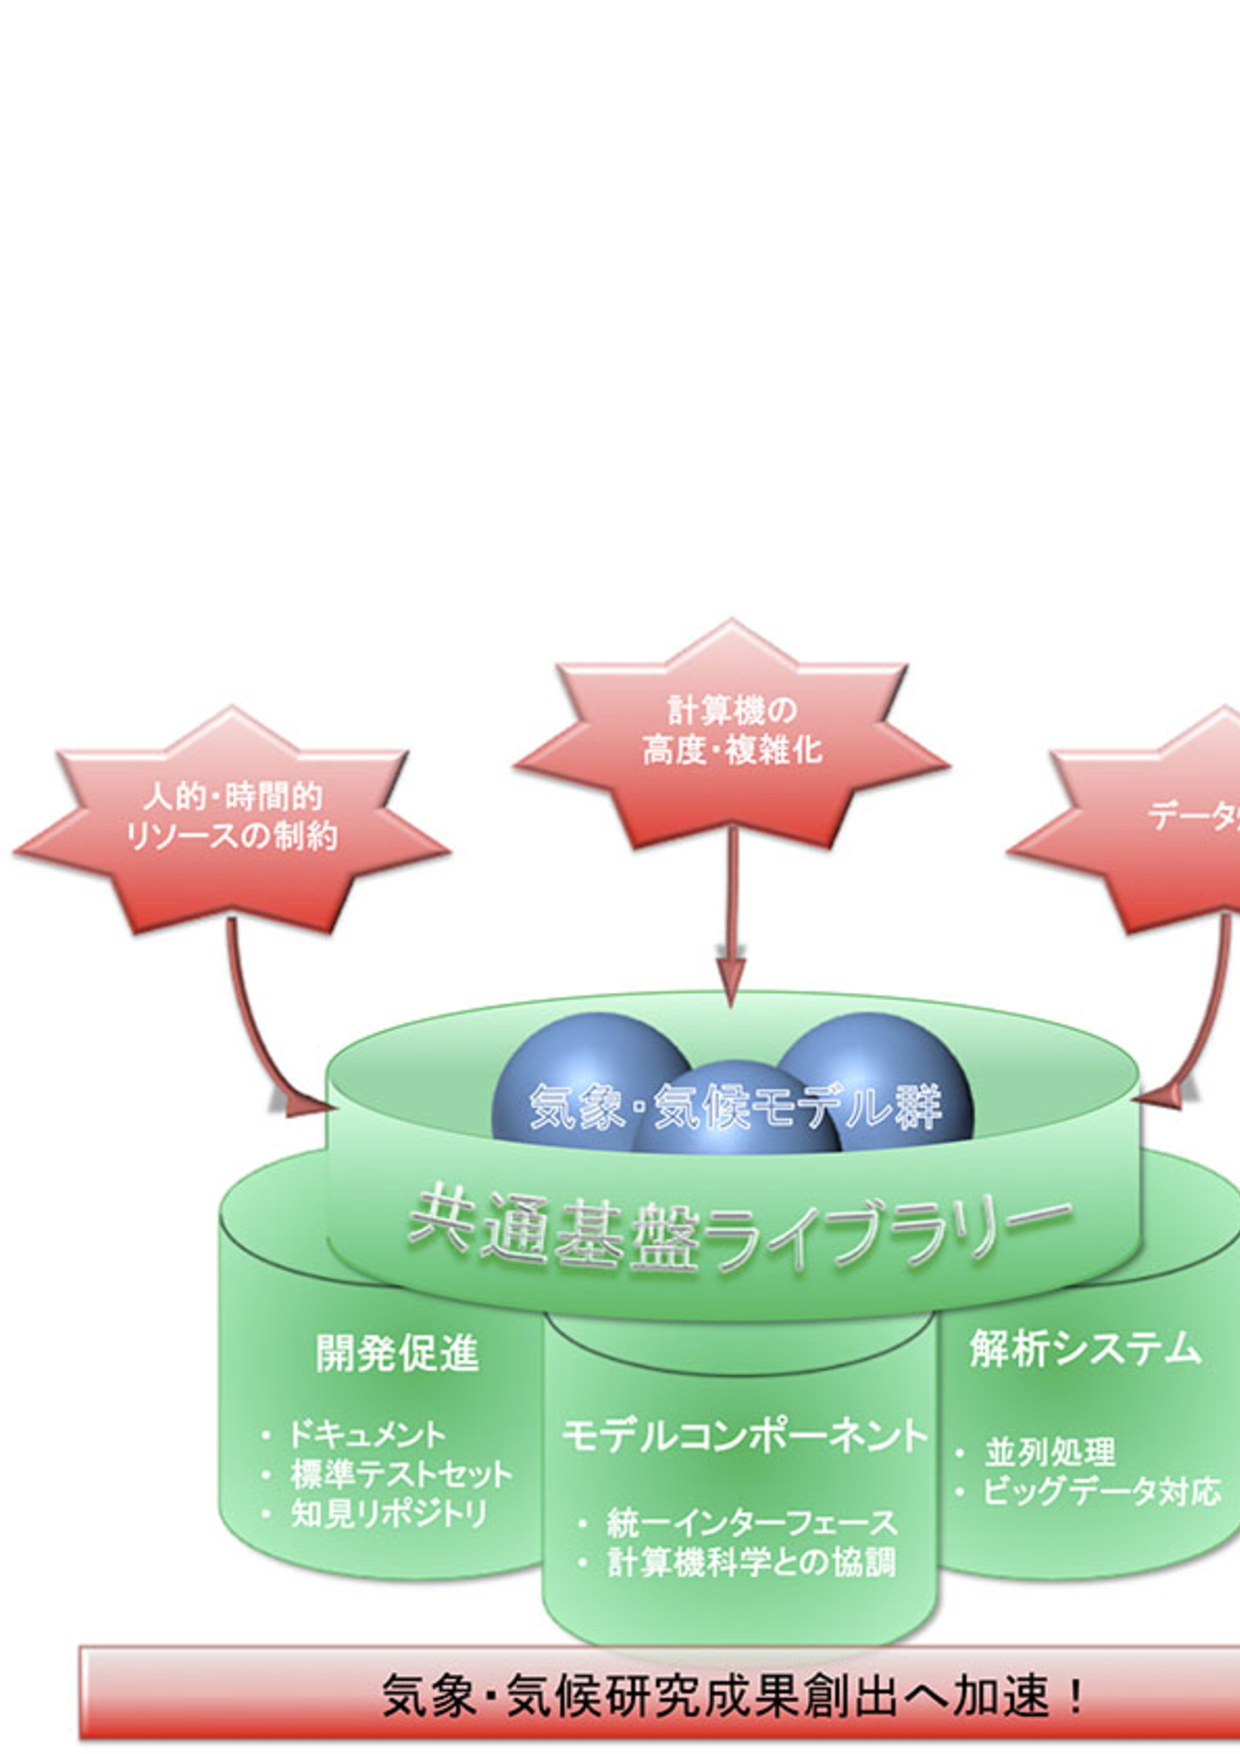
\includegraphics[width=0.9\hsize]{./../../figure/library.pdf}\\
  \caption{Aims of \scalelib}
  \label{fig:scale}
\end{center}
\end{figure}

\scalelib was developed in RIKEN with several outside contributors,
and its improvement and extension continue.
Figure \ref{fig:scale} shows the schematic concept of \scalelib.
As shown in this figure, SCALE aims to resolve various problems.
The development of \scalelib is considered in the context of its wide use
by devices ranging from small PC clusters to next-generation supercomputers.
For this purpose, scientists in meteorology/climate science
and computer science are cooperating.
%This has led to high computational performance of SCALE not only in supercomputers,
%such as the K Computer and the Fujitsu FX10,
%but also for general-purpose commercial computers,
%such as Intel processor-based machines.

\scalerm is a numerical model that fully uses \scalelib.
This model is contained in the \scalelib package,
as shown in Fig. \ref{fig:scale-rm}.
\scalelib manages the parallel processes,
file I/O, and inner-communication.
\scalelib also provides the solver for atmospheric flow ( dynamical core )
and physical processes such as micro-physics and radiation processes.
On the other hand,
\scalerm is constructed by combining functions provided by \scalelib.
\scalerm itself reads the input data of atmospheric status as prognostic variable,
and conducts time-integration.
Users can select a scheme in every component according to simulations they want.

\begin{figure}[hbt]
\begin{center}
  \includegraphics[width=0.9\hsize]{./../../figure/scale.pdf}\\
  \caption{Relationship between the library \scalelib and the model \scalerm}
  \label{fig:scale-rm}
\end{center}
\end{figure}


\section{Structure of \scalerm}  \label{subsec:sturcture_scale_rm}
%--------------------------------------------------------------%
All schemes in all components of \scalelib are available in \scalerm.
The components are categorized into three parts:
framework, dynamical core, and physical processes.
Components with various schemes already implemented
in the current version of \scalerm are listed below\footnote{Refer to \citet{scale_2015},\citet{satoy_2015b}, and \citet{nishizawa_2015} for the details of the model structure and the discretization method.}.

\subsubsection{Framework}
\begin{itemize}
 \item The three-dimensional (3D) Cartesian grid system based on actual distance
 \item 2D domain decomposition by Message Passing Interface (MPI) communication
 \item Several map projections commonly used
 \item Domain nesting system ( one-way, i.e., data transfer from parent domain to child domain. )
   \begin{itemize}
    \item  On-line nesting: concurrent execution of multiple domains).
    \item  Offline nesting: execution of computation in an inner domain after that in an outer domain.
   \end{itemize}
 \item Collective execution system of multiple cases, i.e., bulk job system
 \item \netcdf file I/O based on CF (Climate and Forecast) convention\footnote{\url{http://cfconventions.org/}}
   \begin{itemize}
   \item Selection of {\netcdf}3 and {\netcdf}4 formats
   \end{itemize}
 \item Generation of initial data for an ideal experiment
 \item Generation of topographical and land-use data, converted from external data
 \item Generation of initial and boundary data from external data
   \begin{itemize}
    \item 
      Supporting inputs from the WRF-ARW\footnote{\url{http://www.wrf-model.org/}} and
      \grads \footnote{\url{http://cola.gmu.edu/grads/}} formats.
   \end{itemize}
\end{itemize}

\subsubsection{Dynamical core}
\begin{itemize}
 \item Governing equations: 3D fully compressible non-hydrostatic equations
 \item Spatial discretization: finite volume method
    \begin{itemize}
      \item central advection schemes with 2nd-, 4th-, 6th-order, and 8th-order accuracy
      \item upwind advection schemes with 3rd- , 5th-order, and 7th-order accuracy
    \end{itemize}
 \item Time integration: selection from the ``fully explicit method'' (HEVE)
   or the ``horizontally explicit and vertically implicit methods'' (HEVI)
    \begin{itemize}
      \item \citet{Wicker_2002}'s 3 stage Runge--Kutta scheme with generally 2nd order accuracy
      \item Heun-type 3 stage Runge--Kutta scheme with 3rd order accuracy
      \item 4 stage Runge--Kutta scheme with 4th order accuracy
      \item 7 stage Runge--Kutta scheme with 6th order accuracy (supported only for HEVE)
      \item 11 stage Runge--Kutta scheme with 8th order accuracy (supported only for HEVE)
    \end{itemize}
 \item Guarantee of non-negative value:
    \begin{itemize}
      \item Flux corrected transport method \citep{zalesak_1979}
      \item \citet{Koren_1993}'s filter: available only with the use of the 3rd-order upwind advection scheme
    \end{itemize}
 \item Numerical filter: hyper-viscosity and diffusion with 2nd, 4th, 6th and 8th-order differential operators 
 \item Topography: expressed using terrain-following coordinates
\end{itemize}


\subsubsection{Physical processes}
\begin{itemize}
\item Turbulence process: selectable from among the following
  \begin{itemize}
  \item \citet{smagorinsky_1963} \& \citet{lilly_1962}-type sub-grid scale turbulent model
    with the corrections by \citet{Brown_etal_1994} and \citet{Scotti_1993}
  \item \citet{Deardorff_1980} sub-grid scale turbulent model
  \item MYNN level 2.5 boundary scheme ( \citet{my_1982,nakanishi_2004} )
  \end{itemize}
\item Cloud microphysics: selectable from among the following
  \begin{itemize}
  \item 3-class 1 moment bulk scheme \citep{kessler_1969}
  \item 6-class 1 moment bulk scheme \citep{tomita_2008}
  \item 6-class 2 moment bulk scheme \citep{sn_2014}
  \item spectral bin scheme \citep{suzuki_etal_2010}
  \end{itemize}
\item Radiation process: a k-distribution-based broadband radiation transfer model ( \citet{sekiguchi_2008} )
\item Surface models
  \begin{itemize}
  \item Land model: heat diffusion/bucket model
  \item Ocean model: selectable from among the following
    \begin{itemize}
    \item fixed to initial condition
    \item input from external data
    \item slab model
    \end{itemize}
  \item Urban model: a single-layer canopy model \citep{kusaka_2001}
  \item Heat transfer coefficient at land and in ocean: selectable from among the following
    \begin{itemize}
    \item The bulk method using the universal function \citep{beljaars_1991,wilson_2001}
    \item Louis-type bulk method \citep{uno_1995}
    \end{itemize}
  \end{itemize}
\end{itemize}

\section{Notations used in this document} \label{sec:notation}

This document assumes an execution in the shell ``bash'' on some Unix system.
If your environment is different, replace the commands
by the relevant commands suitable for your environment.
Unless there is a particular remark, this documentation obeys the following notation:

The command-line symbol for execution is expressed by \verb|$| or \verb|#|.
The difference between the two notations is 
in the permission levels of program execution, as shown below:
\begin{verbatim}
 #        <- command by root permission
 $        <- command by user permission
\end{verbatim}

A description enclosed in a rectangle expresses a message generated by the command line, as shown below.
\msgbox{
 -- -- -- -- command-line message\\
 -- -- -- -- -- -- -- -- command-line message\\
 -- -- -- -- -- -- -- -- -- -- -- -- command-line message\\
}

On the other hand, a description enclosed in a polygon with rounded corners means that the description is in an editable file.
\editbox{
 -- -- -- -- description in a file\\
 -- -- -- -- -- -- -- -- description in a file\\
 -- -- -- -- -- -- -- -- -- -- -- -- description in a file\\
}

In this documentation, the FORTRAN namelist and its items are denoted by
\namelist{\it namelist} and \nmitem{\it item_of_namelist}, respectively.



\chapter{インストール} \label{chap:install}
ここでは,日本域を対象とした実事例実験のチュートリアルを通して,SCALE-LESモデルを実行する一連の作業を説明する.


\section{Installation of SCALE-LES}
%####################################################################################

ここでは,SCALE-LESモデルパッケージを含むSCALEライブラリの
インストール方法を説明する.
SCALEライブラリのインストールに必要となるライブラリ環境のインストール方法については,
必要に応じてAppendix \ref{sec:env_setting}を参照して事前にインストールすること.
以降のチュートリアルでは,Ruby DCL/GPhysに含まれるgpviewがインストールされていると想定して描画の説明を行う.
SCALEのインストールにはコマンドライン端末を使う.コマンドラインのシンボル(\verb|$|)があれば、コマンドの実行を示す.


\subsection{Required Environment}
%====================================================================================

\begin{itemize}
  \item {\bf 計算機環境} : Linux互換OS (Mac OS-Xを含む)が動作する環境.
        マルチコアCPU環境以上を推奨する.
        実験サイズによるが4GB以上のメモリがインストールされているマシン環境が好ましい.
  \item {\bf OS} : Linux OS(Fedora, CentOS, SUSE等),Max OS-X.ここではLinux (CentOS7)を使用して説明する.
  \item {\bf コンパイラ} : Fortran 2003をサポートするC,Fortranコンパイラを必要とする.
        GNU 4.6.x以上,Intel compiler 2012以上を推奨する.ここでは,gcc/gfortranを使用して説明する.
  \item {\bf MPIライブラリ} : MPICH2, OpenMPI, Intel MPI等をサポートする.ここではopenMPIを使用して説明する.
  \item {\bf netcdf3 もしくは HDF5/netcdf4} : gzip, szipをサポートするHDF5,
        およびそのHDF5をサポートするnetcdf4を必要とする.
        ただし,netcdf3の環境下ではscaleライブラリが提供する全ての機能をサポートできない可能性がある.
  \item {\bf 描画環境(非必須)} : Dennou Club提供のRuby DCL/GPhysに含まれるgpview,
        もしくはGrads等の描画環境があると計算結果を簡単にチェックできる.gpviewの使用を推奨する.
  \item SCALEは演算性能評価のためにPAPIライブラリを使用が可能です.
        PAPIライブラリがインストールされている環境下では,
        以下で説明するconfigureファイルの編集によってPAPIを適用することができます.
\end{itemize}



\subsection{Building the source code} \label{sec:source_code}
%====================================================================================

\subsubsection{ソースコードの入手}
%-----------------------------------------------------------------------------------

\url{http://scale.aics.riken.jp/download/scale.tar.gz} の安定版ソースコードのtarballをダウンロードすることができる.
ソースコードのtarballファイルを展開すると\verb|scale/|というディレクトリができる.
以降の説明で\verb|${TOPDIR}|は,scaleディレクトリが存在する絶対PATHを差す.

実事例のシミュレーションを行うには,ソースコードに加えて外部データが必要になる.
このチュートリアル用の気象場のデータ,日本領域の地形・土地利用のデータが収められた
\url{http://scale.aics.riken.jp/download/tutorial_data.tar.gz}も入手し,\verb|${TOPDIR}|の下,
つまりscaleディレクトリと同じ場所に展開しておくこと.\\
\begin{itemize}
 \item \verb|tutorial_data/input_atom| に気象場データ,\\
 \item \verb|tutorial_data/input_topo| に地形データ,\\
 \item \verb|tutorial_data/input_landuse| に土地利用データ\\
\end{itemize}
がそれぞれ格納されている.

\verb|tutorial_data|には,本チュートリアルに必要な最低限のデータのみが納めされているため,
その他の設定で実験を行う場合には別途,気象場,地形,および土地利用データが必要となる.


\subsubsection{configure ファイルと環境変数の設定}
%-----------------------------------------------------------------------------------

\verb|scale/sysdep|内にいくつかのコンフィグファイル(\verb|Makedef.***|)が準備されている.
これらの内から自分の環境にあったものを設定する.
ここでは,OSはLinux,gcc/gfortran コンパイラ,およびopenMPIを使用するため,
\verb|"Makedef.Linux-gnu-ompi"|が設定すべきコンフィグファイルである.
自分の環境に合うものがなければ既存ファイルをベースにして作成する必要がある.
\verb|Makedef.***|の\verb|"***"|の部分を下記のように環境変数として設定する.
\verb|.bashrc|などのファイルに記述しておくと便利である.

また、現実実験のための地形データ、
SCALEをコンパイルするのに必要な外部ライブラリについても下記のようにPATHを設定する.
ここでは,Appendix \ref{sec:env_setting}に従ったとして,
HDF5,netcdf4ともに\verb|/usr|の下にインストールされている場合の例を示す.

\begin{verbatim}
 $ export SCALE_SYS="Linux-gnu-ompi"
 $ export HDF5="/usr"
 $ export NETCDF4="/usr"
\end{verbatim}


\subsubsection{コンパイル}
%-----------------------------------------------------------------------------------

下記のディレクトリに移動して,makeコマンドによってコンパイルを行う.
\begin{verbatim}
 $ cd scale-les/test/tutorial/bin
 $ make -j 4
\end{verbatim}

\verb|make|のあとの \verb|"-j 4"| は,並列コンパイルを指示するオプションで,4並列コンパイルを行うことを指示する.
コンパイルを実行する環境によっては並列数を増やすこともできる.

このmakeによってSCALEライブラリ,およびSCALE-LESモデルのコンパイルが行われ,結果として
\verb|scale-les, scale-les_init, scale-les_pp|の3つの実行ファイルが生成されていればコンパイルは成功である.


{\bf 注意点}
\begin{itemize}
\item SCALEライブラリは,scaleのTOPディレクトリ直下の\verb|scale/scalelib/|というディレクトリ内でコンパイルと
アーカイブが行われ,\verb|"./lib"|という名前の隠しディレクトリとして\verb|bin/|ディレクトリ内へコピーされている.\\
\item Debugモードでコンパイルしたい場合や,コンパイルオプションを変更したい場合は,
      \verb|Makedef.***|のファイルを編集してください.
\item 開発版ソースコードをコンパイルしている場合,一部のコンパイラバージョンにおいて
      コンパイルが正常に終了しないケースがあります.そのような場合はぜひSCALE開発チームまでご報告ください.
\end{itemize}



%####################################################################################



\chapter{チュートリアル: 理想実験} \label{chap:tutorial_ideal}
%%%%%%%%%%%%%%%%%%%%%%%%%%%%%%%%%%%%%%%%%%%%%%%%%%%%%%%%%%%%%%%%%%%%%
%  File 31_ideal_exp.tex
%%%%%%%%%%%%%%%%%%%%%%%%%%%%%%%%%%%%%%%%%%%%%%%%%%%%%%%%%%%%%%%%%%%%%
\section{概要} \label{sec:ideal_exp_intro}

本章では、まずSCALE-RMを使ってみるための基本的な操作について説明する。
第\ref{chap:install}章で実行したSCALEのコンパイルが正常に完了しているか
どうかのチェックも兼ねているのでぜひ実施してもらいたい。

%%  ====2章に書いてあるので削除した。
%% \subsubsection{本章を実行するための推奨環境}

%% 本章の説明は、下記の環境を前提として記述している。
%% コンパイラ、ライブラリについては、適宜、使用環境に合わせて読み替えること。

%% \begin{itemize}
%%  \item {\bf CPU} : 物理コアが2コア以上 %[Intel Core i5 2410M 2.3GHz 2コア/4スレッド] %、第\ref{chap:tutorial_real}章は4コアを搭載
%%  \item {\bf Memory} : 512MB以上 %[DDR3-1333 4GB]     %、第\ref{chap:tutorial_real}章は2GB
%%  \item {\bf OS} : Linux OS x86-64  %[CentOS 6.6、CentOS 7.1、openSUSE 13.2のいずれか]
%%  \item {\bf コンパイラ} : GNU コンパイラ(gcc/gfortran)
%%  \item {\bf MPIライブラリ} : openMPI(リポジトリ経由でのインストール)
%% \end{itemize}

本章では、SCALEのコンパイルが正常に終了し、
すでに下記のファイルが生成されているものとして説明を行う。
\begin{alltt} 
  scale-{\version}/scale-rm/test/tutorial/bin/scale-rm
  scale-{\version}/scale-rm/test/tutorial/bin/scale-rm_init
  scale-{\version}/scale-rm/util/netcdf2grads_h/net2g
\end{alltt}
これらに加えて、描画ツールとして\grads を使用する。
gpviewは、結果の確認用に利用することができる。
\grads およびgpview(GPhys)との詳細やインストール方法については、
付録 \ref{sec:env_vis_tools}節を参照のこと。





\section{実行方法} \label{sec:ideal_exp_run}
%====================================================================================

実行の流れとしては、前準備、初期値の作成、モデル本体の実行、
後処理、そして描画といった順番で作業を進める。

\subsection{前準備} \label{subsec:ideal_exp_prepare}
%------------------------------------------------------
チュートリアル理想実験は、\verb|scale-rm/test/tutorial/ideal|の
ディレクトリにて実行する。
\begin{alltt}
  $ cd scale-rm/test/tutorial/ideal
\end{alltt}
次に、このディレクトリに、
SCALEの実行バイナリの静的リンクを張る。
\begin{alltt}
  $ ln -s ../bin/scale-rm       ./
  $ ln -s ../bin/scale-rm_init  ./
\end{alltt}
``\verb|scale-rm|''はモデル本体、
``\verb|scale-rm_init|''は初期値・境界値作成ツールである。
%もし、ここで説明するディレクトリとは異なる場所で実行している場合は、
%リンクを張る時のディレクトリ指定に注意すること。


\subsection{初期値作成} \label{subsec:ideal_exp_init}
%------------------------------------------------------
初期値の作成は、``\verb|scale-rm_init|''に
設定ファイルを与えて実行する。
``\verb|init_R20kmDX500m.conf|''には、
表\ref{tab:setting_ideal}に対応した実験設定が書き込まれている。
この設定ファイルを\verb|scale-rm_init|に与えることで、
設定ファイルの指示に従って大気の成層構造を計算し、
初期擾乱が設定される。


SCALEの基本的な実行コマンドは下記のとおりである。
\begin{alltt}
  $ mpirun  -n  [プロセス数]  [実行バイナリ名]  [設定ファイル]
\end{alltt}
[プロセス数]の部分にはMPI並列で使用したいプロセス数を記述する。
[実行バイナリ]には、\verb|scale-rm|や\verb|scale-rm_init|が入る。
そして、実験設定を記述した設定ファイルを
[設定ファイル]の部分に指定する。
%
例えば、
設定ファイルに\verb|init_R20kmDX500m.conf|を用いて、
2-MPI並列(2つのMPIプロセス)
で\verb|scale-rm_init|を実行する場合、
コマンドは次のようになる。
\begin{alltt}
  $ mpirun  -n  2  ./scale-rm_init  init_R20kmDX500m.conf
\end{alltt}
%
\noindent 実行が成功した場合には、コマンドラインのメッセージは
下記のように表示される。\\

\noindent {\small {\gt
\fbox{
\begin{tabularx}{140mm}{l}
 *** Start Launch System for SCALE-RM\\
 *** Execute preprocess? :  T\\
 *** Execute model?      :  F\\
 *** a single comunicator\\
 *** a single comunicator\\
\end{tabularx}
}}}\\


\noindent この実行によって、
\begin{alltt}
  init_LOG.pe000000
  init_00000101-000000.000.pe000000.nc
  init_00000101-000000.000.pe000001.nc
\end{alltt}
の3つのファイルが、現在のディレクトリ下に作成される。
``init\_LOG.pe000000''には、
コマンドラインには表示されない詳しい実行ログが記録されている。
実行が正常に終了している場合、このLOGファイルの最後に\\

\noindent {\small {\gt
\fbox{
\begin{tabularx}{140mm}{l}
 ++++++ Stop MPI\\
 \\
 *** MPI is peacefully finalized\\
\end{tabularx}
}}}\\

\noindent と記述される。

\verb|init_00000101-000000.000.pe000000.nc|と\verb|init_00000101-000000.000.pe000001.nc|の
2つのファイルは初期値ファイルである。
計算領域全体を2つのMPIプロセスで分割し担当するため、
2つのファイルが生成される。
もし、4-MPI並列で実行すれば、4つの初期値ファイルが生成される。
これらのファイル名の末尾が``.nc''で終わるファイルは
NetCDF形式のファイルであり、
GPhys/Ruby-DCLやncviewといったツールで直接読むことができる。


\subsection{モデル本体の実行} \label{subsec:ideal_exp_run}
%------------------------------------------------------
並列数は、初期値作成のときと同じ数を指定する。
設定ファイルには``\verb|run_R20kmDX500m.conf|''を指定する。
\begin{alltt}
  $ mpirun  -n  2  ./scale-rm  run_R20kmDX500m.conf
\end{alltt}

本書の必要要件にあった計算機であれば、2分程度で計算が終わる。
\noindent この実行によって、\\
\begin{alltt}
  LOG.pe000000
  history.pe000000.nc
  history.pe000001.nc
\end{alltt}
の3つのファイルが、現在のディレクトリ下に作成されているはずである。
``LOG.pe000000''には、
コマンドラインには表示されない詳しい実行ログが記録されている。
実行が正常に終了している場合、このLOGファイルの最後に\\

\noindent {\small {\gt
\fbox{
\begin{tabularx}{140mm}{l}
 ++++++ Stop MPI\\
 \\
 *** MPI is peacefully finalized\\
\end{tabularx}
}}}\\

\noindent と記述される。
``history.pe000000.nc''と``history.pe000001.nc''
の2つのファイルが計算結果が記録されたhistoryファイルである。
2-MPI並列で実行したため、2つのファイルが生成されており、
ファイル形式はNetCDFである。
%``monitor.pe000000''は、計算中にモニタリングしている
%物理変数の時間変化を記録したテキストファイルである。


\section{後処理と描画} \label{sec:ideal_exp_net2g}
%------------------------------------------------------
ここでは、後処理と計算結果の描画方法について説明する。本書のチュートリアルでは、
NetCDF形式の分散ファイルを1つのファイルにまとめ、ダイレクトアクセスが可能な
単純バイナリ形式(\grads 形式)に変換する方法を説明する。
このバイナリ形式は、ユーザーによる結果の解析を容易にする。
%GPhys/Ruby-DCLを使うと
%分割ファイルのまま直接描画することができるが、この方法については\ref{sec:quicklook}節を
%参照してもらいたい。

まず、\ref{sec:source_net2g}節でコンパイルした後処理ツール\verb|net2g|へリンクを張る。
\begin{verbatim}
  $ ln -s ../../../util/netcdf2grads_h/net2g  ./
\end{verbatim}
%もし、ここで説明するディレクトリとは異なる場所で実行している場合は、
%リンクを張る時のディレクトリ指定に注意すること。

\verb|net2g| の実行方法は、基本的に{\scalerm}と同じであり、
\begin{verbatim}
  $ mpirun  -n  [プロセス数]  ./net2g  [設定ファイル]
\end{verbatim}
の形式で実行する。
net2g専用の \verb|net2g_R20kmDX500m.conf|を設定ファイルとして与えて、
次のように実行する。
\begin{verbatim}
  $ mpirun  -n  2  ./net2g  net2g_R20kmDX500m.conf
\end{verbatim}
エラーメッセージがなく、下記のメッセージだけが標準出力へ表示されていれば、正常に変換は完了している。\\

\noindent {\gt
\fbox{
\begin{tabularx}{150mm}{l}
\verb|+++ MPI COMM: Corrective Finalize| \\
\end{tabularx}
}}\\

\noindent net2gの実行には、{\scalerm}の実行時に使用したMPIプロセス数と同じか、
その約数のプロセス数を使用しなければならない。
%HDDの読み書き速度に依存するが、本書の必要要件にあった計算機であれば2分程度で計算が終わる。
この実行によって、実行ディレクトリ下に下記6つのファイルが作成される。
\begin{alltt}
  QHYD_d01z-3d.ctl
  QHYD_d01z-3d.grd
  U_d01z-3d.ctl
  U_d01z-3d.grd
  W_d01z-3d.ctl
  W_d01z-3d.grd
\end{alltt}
「grd」ファイルは、分割ファイルを結合することによって得られる、
ダイレクトアクセス可能の単純バイナリ形式(\grads 形式)である。
一方、「ctl」ファイルは、\grads によって「grd」ファイルを読む込むときに必要な情報を含む。

計算が問題なく完了しているかを確認するため、\grads スクリプト \verb|checkfig_ideal.gs|
を使って作図する。なお、\grads のバージョンによって文法が異なるため、
警告が出る場合には\grads スクリプトを適宜変更されたい。
\begin{verbatim}
  $ grads -blc checkfig_ideal.gs
\end{verbatim}
作図が成功すると、下記の図が生成される。
\begin{verbatim}
   ideal_QHYD.png
   ideal_W.png
\end{verbatim}
シミュレーションと後処理が成功していれば、図\ref{fig_ideal}と同じ図が得られる。

\begin{figure}[t]
\begin{center}
  \includegraphics[width=0.7\hsize]{./figure/ideal_qhyd.eps}\\
  \includegraphics[width=0.7\hsize]{./figure/ideal_W.eps}\\
  \caption{積分開始から 1200 秒(20 分)後の Y=750 mにおける東西-鉛直断面図;
           カラーシェードは、(a)において全質量に対する凝結物の質量比、
           (b)において鉛直速度を表す。ベクトルは東西-鉛直断面内の風の流れを表す。}
  \label{fig_ideal}
\end{center}
\end{figure}


他の変数についてもバイナリデータに変換したい場合には、
\verb|net2g_R20kmDX500m.conf|の\namelist{VARI}の\nmitem{VNAME} に必要な変数を追加すればよい。\\

\noindent {\small {\gt
\ovalbox{
\begin{tabularx}{150mm}{l}
\verb|&VARI|\\
\verb| VNAME       = "U","W","QHYD"|\\
\verb|/|\\
\end{tabularx}
}}}\\

\noindent
historyファイルに出力されている変数は、{\netcdf} の\verb|ncdump| などを
使えば簡単に確認できる。net2gの詳しい使用方法は、第\ref{sec:net2g}節を参照されたい。





\section{Guideline for further study} \label{sec:ideal_exp_last}

In this chapter,
the method for the execution of \scalerm was explained by using a simple ideal experiment. We recommend studying methods of changing the model resolution, the calculation domain, and the number of MPI processes for further study.  With regard to the ideal experiment, several files of other configurations,  e.g., to increase resolution, the number of domains, and the physical scheme, are prepared in the directory ``sample'' under the same directory as was used in this experiment.  These configuration files are useful to change such configurations.  Moreover, various ideal experimental settings  have been prepared in the directory ``\verb|scale-rm/test/case|.'' For some ideal experiments,  it may be necessary to carry out the ``make'' command again in the same directory as in the configuration file  because some test cases need special source codes according to their experimental settings. The procedures for the generation of the initial conditions and those for simulation execution are the same as in the tutorial in this chapter.

It is important to study the method for the configuration of physical processes, such as cloud microphysics, radiation, and turbulence schemes. Methods to alter them in detail are described in Chapter \ref{chap:basic_usel}.



\chapter{チュートリアル: 現実実験} \label{chap:tutorial_real}
%-------------------------------------------------------%
\section{Overview} \label{sec:tutrial_real_intro}
%-------------------------------------------------------%
In this chapter, the basic execution procedure of the real atmospheric experiment is described using a simple case according to the workflow in Fig. \ref{fig:howto}.
\begin{enumerate}
\item Preparations for input data. The input data must be prepared by users themselves.
\item \texttt{pp}:   Making topographical data
\item \texttt{init}: Making initial and boundary data
\item \texttt{run}:  Executing the simulation
\item \texttt{net2g}: Converting {\netcdf} output data to {\grads} format ( optional )
\end{enumerate}
Hereinafter, the absolute path \texttt{scale-{\version}/scale-rm/test/tutorial/} is denoted by\\
\verb|${Tutorial_DIR}|.

\begin{figure}[tb]
\begin{center}
  \includegraphics[width=0.9\hsize]{./figure/real_procedure.eps}\\
  \caption{\scalerm procedure of model execution}
  \label{fig:howto}
\end{center}
\end{figure}

The settings for the calculation domain used in this tutorial are given in Table \ref{tab:grids}.
Figure \ref{fig:tutrial_real_domain} shows the target domain.
Since this tutorial focuses on learning how to conduct 
real atmospheric experiments using \scalerm quickly,
the experiment is designed to be completed in a short time.
Note that this setting may not be appropriate as a physically valid experiment;
e.g., there is no cumulus parameterization in this simulation, even though the horizontal resolution is 20 km.

\begin{table}[tb]
\begin{center}
  \caption{Overview of experimental settings}
  \label{tab:grids}
  \begin{tabularx}{150mm}{|l|X|} \hline
    \rowcolor[gray]{0.9} Item & Configuration \\ \hline
    MPI process decomposition (east-west $\times$ north-south) & 2 $\times$ 2 (total: 4 processes) \\ \hline
    Number of horizontal grids (east-west $\times$ north-south) & 90 $\times$ 90  \\ \hline
    Number of vertical layers   & 36                   \\ \hline
    Horizontal grid intervals   & $\Delta x  = \Delta y = $ 20km       \\ \hline
    Integration period & July 14, 2007, 18UTC - July 15 00UTC (6 hour integration) \\ \hline
    Time step & 90 s/step (total:240 steps) \\ \hline
  \end{tabularx}
\end{center}
\end{table}

\begin{figure}[tb]
\begin{center}
  \includegraphics[width=1.0\hsize]{./figure/real_domain.eps}\\
  \caption{Topographical and land-ocean distribution in the domain}
  \label{fig:tutrial_real_domain}
\end{center}
\end{figure}



%-------------------------------------------------------%
\section{実験セットの準備} \label{sec:tutrial_real_prep}
%-------------------------------------------------------%

現実大気実験は、理想実験よりも実行手続きや必要なファイルが多く、
プレ処理\verb|pp|、初期値作成\verb|init|、シミュレーション実行\verb|run|
で使用する設定ファイル(**.conf)内の実験設定を統一する必要がある。
準備段階でのファイルの不足や設定の不一致はモデルが正常に動かない原因となる。
これを回避するため、
現実実験の実行に必要なファイル一式を用意するためのツールが用意されている。
まずはじめに、
以下のディレクトリーに移動し、
次の手続きにより現実大気実験のためのファイル一式を用意する。
\begin{alltt}
 $ cd scale-{\version}/scale-rm/test/tutorial/real/
 $ ls 
    Makefile : 実験セット一式作成のためのMakefile
    README   : 実験セット一式作成ツールに関するREADME
    USER.sh  : 実験設定の記述
    config/  : 実験セット一式作成つーつのためのファイル(ユーザーは基本書き換えない)
    data/    : チュートリアルのためのツール類
    sample/  : サンプルプログラム
    tools/   : チュートリアル用の入力大気データ用意のためのツール(基本各自で準備)
 $ make
 $ ls experiment/    : make により追加
   init/  net2g/  pp/  run/
\end{alltt}
\verb|make|を実行すると、\verb|USER.sh|に記述された設定に従って、
\verb|experiment|ディレクトリの下に実験セットが作成される。
実験セット一式準備ツールに関する詳しい説明については、第\ref{sec:basic_makeconf}節を参照いただきたい。
なお、\verb|sample|ディレクトリにはネスティングの際に利用できるファイルが用意されており、
必要に応じて参考にされたい。

これ以降の説明では、\texttt{scale-{\version}/scale-rm/test/tutorial/}の絶対PATHを
\verb|${Tutorial_DIR}|と示すこととする。


\input{43_real_exp_pp}
%-------------------------------------------------------%
\section{初期値・境界値データの作成:init} \label{sec:tutrial_real_init}
%-------------------------------------------------------%

init では、SCALE計算に必要な初期値・境界値データを作成する。
まず、initディレクトリへ移動する。
\begin{verbatim}
 $ cd ${Tutorial_DIR}/real/init
\end{verbatim}
ディレクトリの中には、\verb|init.conf|という名前の設定ファイルが準備されている。
\verb|pp.conf|と同様に、実験設定に合わせて、この\verb|init.conf|を書き換える必要があるが、
チュートリアル用の\verb|init.conf|ファイルは表\ref{tab:grids}の設定に
すでに合わせてある。
初期値・境界値データの作成には前節で作成した地形・土地利用データを利用する。
これは、\verb|init.conf|の中で、下記のように相対PATHを用いて参照するように設定されている。\\

\noindent {\gt
f\ovalbox{
\begin{tabularx}{140mm}{l}
\verb|&PARAM_TOPO| \\
\verb|   TOPO_IN_BASENAME = "../pp/topo_d01",| \\
\verb|/| \\
 \\
\verb|&PARAM_LANDUSE| \\
\verb|   LANDUSE_IN_BASENAME  = "../pp/landuse_d01",| \\
\verb|/| \\
\end{tabularx}
}}\\

\noindent その他に\verb|init.conf|の設定の中で特に確認してほしい項目は、
\namelist{PARAM_MKINIT_REAL}である。\\

\noindent {\gt
\ovalbox{
\begin{tabularx}{140mm}{l}
\verb|&PARAM_MKINIT_REAL| \\
\verb|   BASENAME_BOUNDARY    = "boundary_d01",|   {\small ← 境界値データの出力名} \\
\verb|   FILETYPE_ORG         = "GrADS",| \\
\verb|   NUMBER_OF_FILES      = 3,|                      {\small ← 読み込むファイルの数} \\
\verb|   BOUNDARY_UPDATE_DT   = 21600.D0,|           {\small ← 入力データの時間間隔} \\
\verb|   INTERP_SERC_DIV_NUM  = 20,|                   {\small ← 内挿計算用のチューニングパラメータ} \\
\verb|   PARENT_MP_TYPE       = 3,| \\
\verb|   USE_FILE_DENSITY     = .false.,|          {\small ← 親モデルの大気密度データを使うか} \\
\verb|   USE_FILE_LANDWATER   = .true.,|           {\small ← 親モデルの土壌水分データを使うか} \\
\verb|   INTRP_LAND_SFC_TEMP  = "mask",|           {\small ← 親モデルの欠測値処理方法} \\
\verb|   INTRP_LAND_TEMP      = "fill",| \\
\verb|   INTRP_LAND_WATER     = "fill",| \\
\verb|   INTRP_OCEAN_SFC_TEMP = "mask",| \\
\verb|   INTRP_OCEAN_TEMP     = "mask",| \\
\verb|/| \\
\end{tabularx}
}}\\

\noindent \nmitem{FILETYPE_ORG}は入力する気象場データのファイルフォーマットに
関するパラメータを設定しており、ここでは
grads形式のデータを読み込むことを指定している。
詳細な設定ファイルの内容については、付録\ref{app:namelist}を参照されたい。

次に、コンパイル済みのバイナリをinitディレクトリへリンクする。
\begin{verbatim}
  $ ln -s ../../bin/scale-rm_init ./
\end{verbatim}
第\ref{sec:tutrial_real_prep_fnl}節で作成した入力データに、
initディレクトリの中に準備されている\verb|"gradsinput-link_FNL.sh"|を用いてリンクをはる。
\begin{verbatim}
  $ sh gradsinput-link_FNL.sh
\end{verbatim}
下記のgrads形式のファイルにリンクが張れれば成功である。\\

\noindent {\gt
\fbox{
\begin{tabularx}{140mm}{l}
\verb|FNLatm_00000.grd -> ../tools/FNL_output/200707/FNLatm_2007071418.grd| \\
\verb|FNLatm_00001.grd -> ../tools/FNL_output/200707/FNLatm_2007071500.grd| \\
\verb|FNLatm_00002.grd -> ../tools/FNL_output/200707/FNLatm_2007071506.grd| \\
\verb|FNLatm_00003.grd -> ../tools/FNL_output/200707/FNLatm_2007071512.grd| \\
\verb|FNLland_00000.grd -> ../tools/FNL_output/200707/FNLland_2007071418.grd| \\
\verb|FNLland_00001.grd -> ../tools/FNL_output/200707/FNLland_2007071500.grd| \\
\verb|FNLland_00002.grd -> ../tools/FNL_output/200707/FNLland_2007071506.grd| \\
\verb|FNLland_00003.grd -> ../tools/FNL_output/200707/FNLland_2007071512.grd| \\
\verb|FNLsfc_00000.grd -> ../tools/FNL_output/200707/FNLsfc_2007071418.grd| \\
\verb|FNLsfc_00001.grd -> ../tools/FNL_output/200707/FNLsfc_2007071500.grd| \\
\verb|FNLsfc_00002.grd -> ../tools/FNL_output/200707/FNLsfc_2007071506.grd| \\
\verb|FNLsfc_00003.grd -> ../tools/FNL_output/200707/FNLsfc_2007071512.grd| \\
\end{tabularx}
}}\\






次に、陸面の変数を用意するのに必要なパラメータファイルにリンクをはる。
\begin{verbatim}
 $ ln -s ../../../data/land/* ./   <- 陸面スキーム用のパラメータファイル
\end{verbatim}
準備が整ったら、4つのMPIプロセスを使用してinitを実行する。
\begin{verbatim}
 $ mpirun -n 4 ./scale-rm_init init.conf
\end{verbatim}

正常にジョブが終了すると、
\begin{verbatim}
 $ ls
  boundary_d01.pe000000.nc
  boundary_d01.pe000001.nc
  boundary_d01.pe000002.nc
  boundary_d01.pe000003.nc
  init_d01_20070714-180000.000.pe000000.nc
  init_d01_20070714-180000.000.pe000001.nc
  init_d01_20070714-180000.000.pe000002.nc
  init_d01_20070714-180000.000.pe000003.nc
  init_LOG_d01.pe000000
\end{verbatim}
が作成される。
\verb|boundary_d01.pe######.nc|は境界値データ、
\verb|init_d01_20070714-180000.000.pe######.nc|は初期値データ、
\verb|init_LOG_d01.pe######|はログファイルである。
\verb|######|はMPIプロセス番号を表している。


%% サポート外
%% \vspace{1cm}
%% \noindent {\Large\em OPTION} \hrulefill \\
%% gpviewがインストールされている場合,作成された初期値と境界値が
%% 正しく作成されているかどうかを確認することが出来る。
%% 正しく作成されていれば、図 \ref{fig:init}と同じように描かれる。

%% \begin{verbatim}
%% $ gpvect --scalar --slice z=1500 --nocont --aspect=1 --range=0.002:0.016          \
%%          --xintv=10 --yintv=10 --unit_vect init_d01_20140810-000000.000.pe00*@QV      \
%%          init_d01_20140810-000000.000.pe00*@MOMX init_d01_20140810-000000.000.pe00*@MOMY
%% \end{verbatim}


%% \begin{figure}[h]
%% \begin{center}
%%   \includegraphics[width=0.7\hsize]{./figure/init_qv-momxy.eps}\\
%%   \caption{チュートリアル実験の高さ1500mにおける初期場の様子.カラーシェードは比湿,
%%            ベクトルは水平運動量フラックスを表している.}
%%   \label{fig:init}
%% \end{center}
%% \end{figure}


\input{45_real_exp_run}
\section{結果を描画する:net2g}
\label{sec:quicklook}
%####################################################################################

SCALEモデルの出力ファイルは、MPIプロセス毎に計算領域が分割されて、別々のファイルとして出力される。
それぞれのファイルフォーマットは気候・予報(CF)メタデータ規約
に対応したNetCDF4形式である\footnote{gpviewがインストールされている場合、gpviewを使って作図することも出来る。
gpviewならばhistoryデータを変換することなく直接作図することができるため、クイックチェックに適している。}。
ここでは、1) プロセス毎に分割されたNetCDFファイルを
gradsで扱えるように1つのバイナリーファイルにまとめ、
2) 作図して結果の確認を行う。


\subsubsection{GrADSバイナリーに変換}
%-----------------------------------------------------------------------------------
プロセスごとに分割されたNetCDF形式のhistoryファイルから
GrADSバイナリー変換するには、\verb|netcdf2grads_h|を使用する。
詳細な使用方法は \ref{sec:net2g}節を参照頂くこととして、
ここでは最低限の手続きのみ説明する。まず、net2gディレクトリへ移動する。
\begin{verbatim}
 $ cd ${Tutorial_DIR}/real/net2g
\end{verbatim}

\ref{sec:source_net2g}節でコンパイルしたバイナリーファイルにリンクを張る。
\begin{verbatim}
 $ ln -s ../../../../util/netcdf2grads_h/net2g ./
\end{verbatim}
ここでは例として、2次元変数であるMSLP、PRECを、
3次元変数として850hPa,500h,200hPa面のU、Vを変換する.
2次元変数のための設定ファイルは\verb|net2g.2d.conf|に、
3次元変数のための設定ファイルは\verb|net2g.3d.conf|に用意している。

\verb|netcdf2grads_h|実行時のプロセス数は、
計算実行時に使用したプロセス数の約数である必要がある。
ここでは、計算に用いたのと同じ4プロセスを使用することとする。
\begin{verbatim}
 $ mpirun -n 4 ./net2g net2g.2d.conf
 $ mpirun -n 4 ./net2g net2g.3d.conf
\end{verbatim}
%両方とも数秒程度で終了する。
エラーメッセージがなく、次のメッセージだけが標準出力へ表示されて終了すれば変換完了である。\\

\noindent {\gt
\fbox{
\begin{tabularx}{140mm}{l}
\verb|+++ MPI COMM: Corrective Finalize| \\
\end{tabularx}
}}\\

成功すれば、下記のファイルが作成される。
\begin{verbatim}
  MSLP_d01z-2d.ctl
  MSLP_d01z-2d.grd
  PREC_d01z-2d.ctl
  PREC_d01z-2d.grd
  U_d01z-3d.ctl
  U_d01z-3d.grd
  V_d01z-3d.ctl
  V_d01z-3d.grd
\end{verbatim}


\subsubsection{計算結果の確認}
%-----------------------------------------------------------------------------------
現在のバージョンの\verb|netcdf2grads_h|では、
SCALEのXY格子座標で、ctlファイルを作成する。
今後、緯度経度座標で描画するためのctlファイルを
出力できるようにする予定であるが、
現バージョンは未対応のため、
緯度経度座標で作図するためのctlを別途用意している。
\begin{verbatim}
  MSLP_d01z-2d_lcc.ctl
  PREC_d01z-2d_lcc.ctl
  U_d01z-3d_lcc.ctl
  V_d01z-3d_lcc.ctl
\end{verbatim}

計算結果確認用の図を作成するための
スクリプト\verb|checkfig.gs|を使って作図する。
\begin{verbatim}
 $ grads -blc checkfig.gs
\end{verbatim}
成功すると、下記の図が作成される。
なお、GrADSのバージョンによって文法が異なるので、
Warningが出る場合は、適宜変更する。
\begin{verbatim}
  real_mslp.png
  real_prec.png
  real_wind.png
\end{verbatim}
計算と変換が成功していれば、下記と同じ図が描画される。

\begin{figure}[h]
\begin{center}
  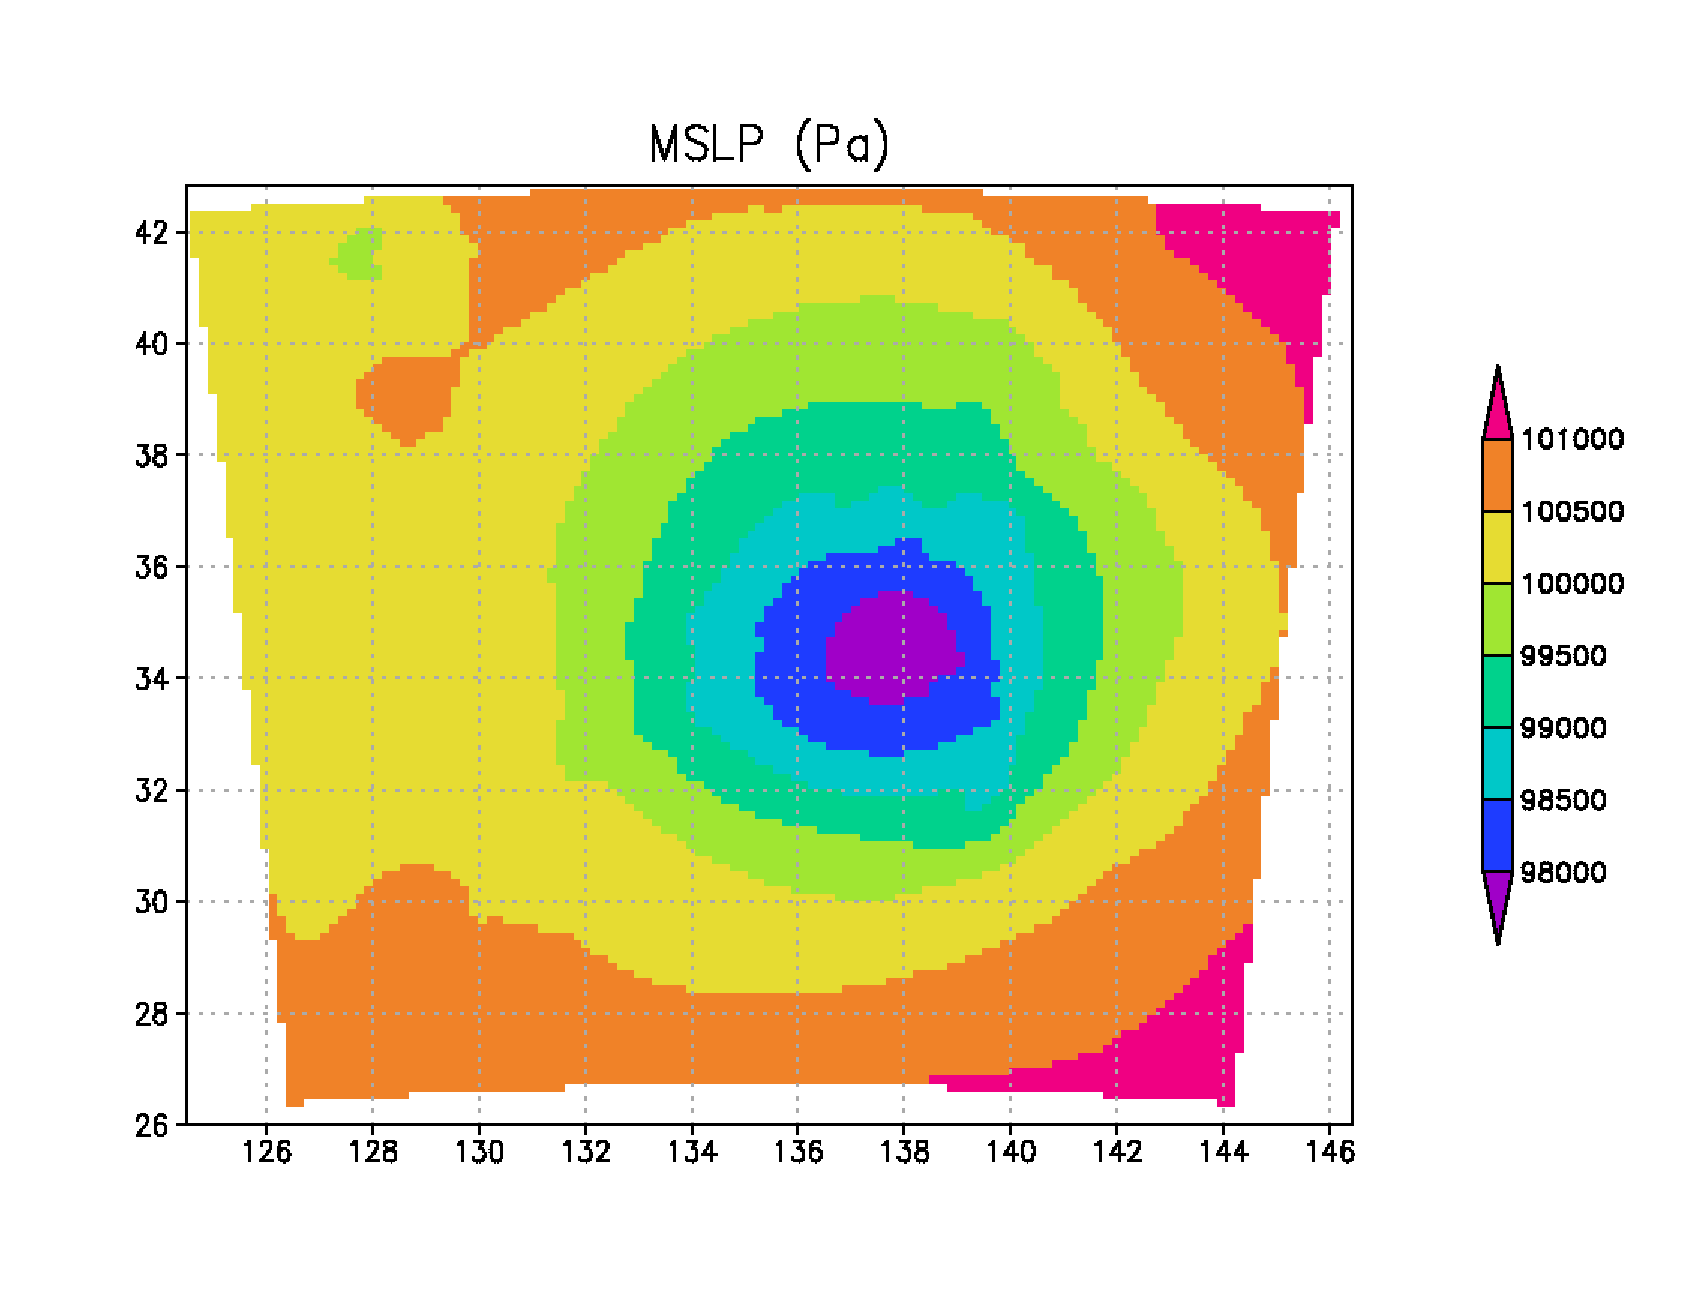
\includegraphics[width=0.55\hsize]{./figure/real_mslp.eps}\\
  \caption{計算開始から6時間後の海面更正気圧}
  \label{fig:real_mslp}
\end{center}
\begin{center}
  \includegraphics[width=0.55\hsize]{./figure/real_prec.eps}\\
  \caption{計算開始から6時間後の降水フラックス}
  \label{fig:real_prec}
\end{center}
\begin{center}
  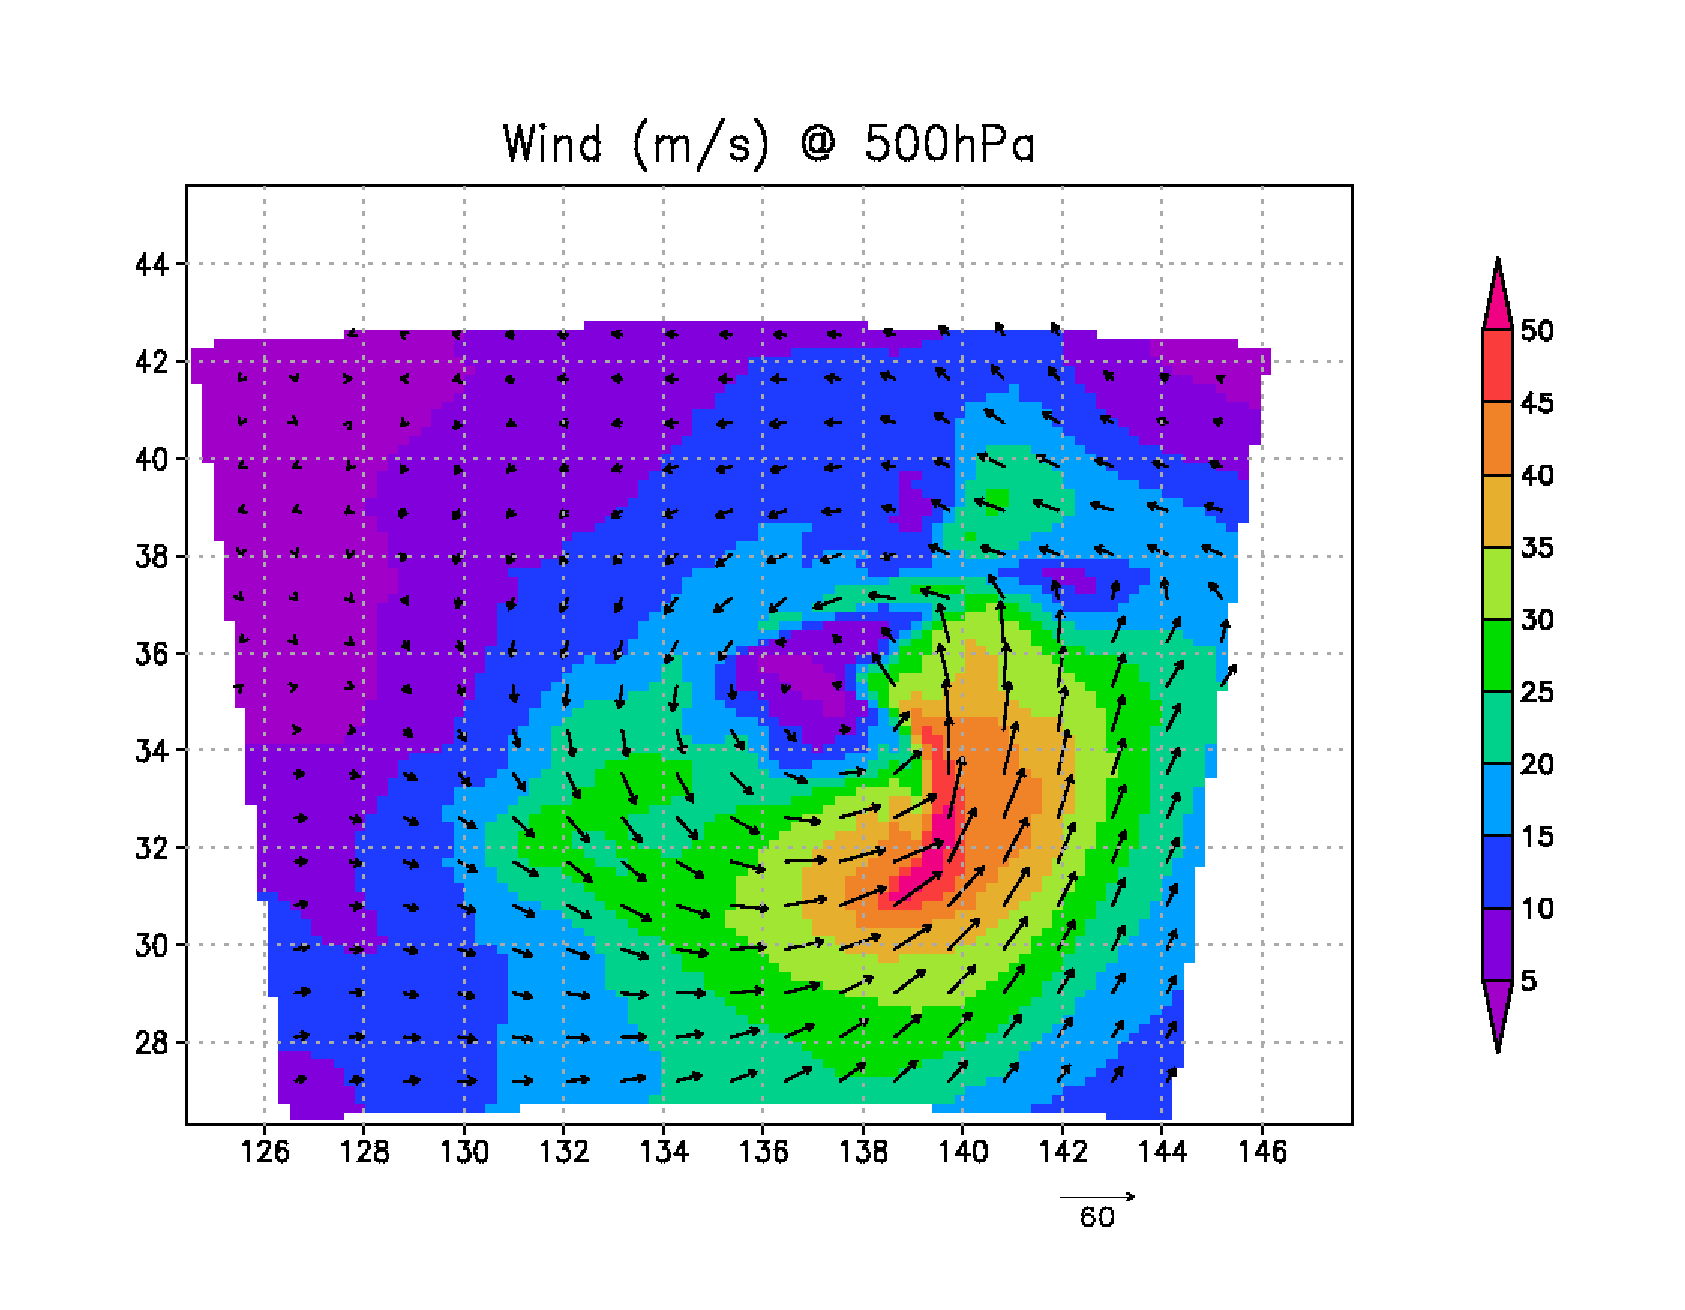
\includegraphics[width=0.55\hsize]{./figure/real_wind.eps}\\
  \caption{計算開始から6時間後の500hPaの風速と風ベクトル}
  \label{fig:real_wind}
\end{center}
\end{figure}





\chapter{各種設定: 基礎編} \label{chap:basic_usel}
\section{概要} \label{chap:basic_usel_intro}

この章では、チュートリアルから発展して、基本的な様々な設定が出きるように、
各種設定を網羅的に記述している。
各節で閉じており、以下の項目に記述されており、辞書代わりに使ってほしい。

{%\small
\begin{center}
\begin{tabular}[h]{ll}\hline
対象計算領域の設定 & 第\ref{sec:domain} 節 \\
計算領域と解像度、格子点数、MPIプロセスの関係 & 第\ref{subsec:relation_dom_reso} 節 \\
計算領域の設定 & 第\ref{subsec:relation_dom_reso2} 節 \\
MPIプロセス数 & 第\ref{subsec:relation_dom_reso3} 節 \\
水平・鉛直格子数 & 第\ref{subsec:relation_dom_reso4} 節 \\
水平・鉛直格子間隔 & 第\ref{subsec:gridinterv} 節 \\
緩和領域の設定 & 第\ref{sec:buffer} 節 \\
積分時間と積分時間間隔の設定 & 第\ref{sec:timeintiv} 節 \\
出力変数の追加・変更 & 第\ref{sec:output} 節\\
力学スキームの設定 & 第\ref{sec:atmos_dyn} 節 \\
数値解法  & 第\ref{subsec:atmos_dyn_sover} 節 \\
時間・空間差分スキーム & 第\ref{subsec:atmos_dyn_scheme} 節 \\
物理スキームの設定 & 第\ref{chap:basic_usel_physics} 節 \\
雲微物理スキーム & 第\ref{chap:basic_usel_microphys} 節 \\
乱流スキーム & 第\ref{chap:basic_usel_turbulence} 節 \\
放射スキーム & 第\ref{chap:basic_usel_radiation} 節 \\
地表面(大気下端境界) & 第\ref{chap:basic_usel_surface} 節 \\
海洋モデル & 第\ref{chap:basic_usel_ocean} 節 \\
陸面モデル & 第\ref{chap:basic_usel_land} 節 \\
都市モデル(大気-都市面フラックス) & 第\ref{chap:basic_usel_urban} 節 \\
\hline
\end{tabular}
\end{center}
}

%\section{対象計算領域の設定} \label{sec:domain}
\section{\SecBasicDomainSetting} \label{sec:domain}
%=======================================================================

\subsubsection{\SubsecRelationOfResoGridProcess} \label{subsec:relation_dom_reso}
各設定を行う前に、\scalerm での計算領域、解像度、格子点数、MPIプロセスの関係を整理しておく。
計算領域は、水平格子間隔と格子点数を指定することで決定されるようになっている。
図\ref{fig:domain}は、
計算領域、水平格子間隔、格子数、及びMPIプロセス数の関係を示している。
水平方向に2次元の領域分割を行うことで並列化がなされている。

これらは、\namelist{PARAM_INDEX}内の\nmitem{IMAX}、\nmitem{JMAX}、
\namelist{PARAM_PRC}内の\nmitem{PRC_NUM_X}、\nmitem{PRC_NUM_Y}で
水平格子間隔については、\namelist{PARAM_GRID}内の\nmitem{DX}、\nmitem{DY}で
設定する。

ここで、注意すべきことは、「指定する格子点数は各プロセスが受け持つ値」であることである。
設定する格子数(\nmitem{IMAX}, \nmitem{JMAX}, \nmitem{KMAX})は、
1つのMPIプロセスが担当する格子点数を与える仕様となっている。
すなわち、計算領域は、水平格子間隔、格子点数とともに
各方向のMPIプロセス数を考慮して決定する必要がある。

図\ref{fig:domain}に示すように、
MPIプロセス数が$n$(=\verb|PRC_NUM_X|$\times$\verb|PRC_NUM_Y|)の時、
計算領域は、$x$方向に\verb|PRC_NUM_X|個、$y$方向に\verb|PRC_NUM_Y|個に分割される。
以上の関係から、計算領域全体のそれぞれの方向の格子点数および総格子点数は、
\begin{eqnarray}
&& 領域内{\XDIR} の格子数 = \left(\verb|IMAX| \times \verb|PRC_NUM_X|\right)
   \times (\verb|KMAX| )  \label{eq:xgridnum}\\
&& 領域内{\YDIR}の格子数 = \left(\verb|JMAX| \times \verb|PRC_NUM_Y|
   \times (\verb|KMAX|\right)  \label{eq:ygridnum}\\
&& 領域内の総格子数 = \left(\verb|IMAX| \times \verb|PRC_NUM_X|\right)
   \times (\verb|JMAX| \times \verb|PRC_NUM_Y|)
   \times (\verb|KMAX| )  \nonumber
\end{eqnarray}
の関係となる。
ここで、\verb|KMAX|は、鉛直方向の格子点数であり、
\namelist{PARAM_INDEX}内の項目で指定されている。
次節以降では、MPIプロセス数、格子数、格子間隔、
それぞれの設定方法について詳しく説明する。

\begin{figure}[h]
\begin{center}
  \includegraphics[width=0.8\hsize]{./figure/domain_decomposition.eps}\\
  \caption{計算領域に対する、水平格子間隔(DX, DY)、1MPIプロセスあたりの格子数(IMAX, JMAX)、MPIプロセス数(PRC\_NUM\_X, PRC\_NUM\_Y)の関係。
水色領域は、ある1つのMPIプロセスが担当する領域。}
  \label{fig:domain}
\end{center}
\end{figure}

\subsection{\SubsecDomainSetting} \label{subsec:relation_dom_reso2}

前節で述べた関係が理解できれば、領域の設定は容易である。
すなわち、式(\ref{eq:xgridnum},\ref{eq:ygridnum})を使って、
\begin{eqnarray}
&& {\XDIR} の領域の長さ = {\XDIR} の格子点数 \times \verb|DX| \nonumber\\
&& {\YDIR}の領域の長さ = {\YDIR}の格子点数 \times \verb|DY| \nonumber
\end{eqnarray}
となる。ここで、\nmitem{DX,DY}は、後述するように
\namelist{PRAM_GRID}で指定されるものである。
逆算して、解像度と領域の大きさをを決めて、MPIプロセス数が決まると、
ローカルな領域の格子点数が決まる。

\subsection{\SubsecMPIProcess} \label{subsec:relation_dom_reso3}

MPIプロセス数は、設定ファイルの\namelist{PARAM_PRC}で指定する。
先に述べた通り、\scalerm の入出力ファイルは、MPIプロセス毎に分割されている。
そのため、MPIプロセス数を変更すると分割ファイル数も必ず変わることになる。
従って、例えば、2-MPI並列用に作成した初期値ファイルは、
4-MPI並列のモデル実行には使用できない。
MPIプロセス数を変更するには、
\verb|pp_***.conf|、\verb|init_***.conf|、\verb|run_***.conf| の
すべてを編集・変更し、\verb|pp|, \verb|init| から行う必要がある。\\

\noindent {\small {\gt
\ovalbox{
\begin{tabularx}{140mm}{lX}
\verb|&PARAM_PRC| & \\
\verb| PRC_NUM_X       = 2,| & ; {\XDIR} (東西方向)のMPI並列分割数 \\
\verb| PRC_NUM_Y       = 1,| & ; {\YDIR}(南北方向)のMPI並列分割数 \\
\verb|/|\\
\end{tabularx}
}}}\\


全MPIプロセス数は、\verb|PRC_NUM_X| $\times$ \verb|PRC_NUM_Y|  となり、
上記の例では、$x$方向に2分割、$y$方向に1分割(分割なし)の
2-MPI並列ということになる。

実行時にMPIコマンドに指定するMPIプロセス数は、
この総MPIプロセス数を指定しなければならない。
この条件を満たさない場合は、下記のメッセージが
LOGファイルなどに出力されて計算は行われず、直ちに終了する。

\noindent {\small {\gt
\ovalbox{
\begin{tabularx}{140mm}{l}
\verb|xxx total number of node does not match that requested. Check!| \\
\end{tabularx}
}}}\\





\subsection{\SubsecGridNumSettng} \label{subsec:relation_dom_reso4}
%-----------------------------------------------------------------------

格子数の設定は、設定ファイル(\verb|***.conf|)の\namelist{PARAM_INDEX}で行う。
以下で設定する水平格子数の値は、1つのMPIプロセス当たりの値であることに注意が必要である。\\

\noindent {\small {\gt
\ovalbox{
\begin{tabularx}{140mm}{lX}
\verb|&PARAM_INDEX| & \\
\verb| KMAX = 97,|  & 鉛直層数 \\
\verb| IMAX = 20,|  & プロセスあたりの{\XDIR} の格子点数 \\
\verb| JMAX = 25,|  & プロセスあたりの{\YDIR}の格子点数 \\
\verb|/|\\
\end{tabularx}
}}}\\



\subsection{\SubsecGridIntvSettng} \label{subsec:gridinterv}
%-----------------------------------------------------------------------
\scalerm では、水平方向には格子点の位置を均等間隔に設定する。
鉛直方向には均等間隔でも任意の格子点位置を直接指定することもできる。
以下で説明する
\textcolor{red}{\bf 格子間隔の設定は、pp\_***.conf、init\_***.conf、run\_***.confの
設定ファイルの間で一致させなければならないことに注意が必要である。}
以下で設定する値は、MPIプロセス当たりの値であることに注意が必要である。

%-----------------------------------------------------------------------&
第\ref{subsec:buffer}節で述べる緩和領域を覗き、
水平格子間隔は等間隔でしか設定できない。
鉛直格子間隔については、任意に定義することが可能である。
すべての方向について等間隔で設定する場合には、以下のように
設定ファイルの\namelist{PARAM_GRID}の\nmitem{DX,DY,DZ}に
それぞれ、東西、南北、鉛直方向の格子間隔を指定する。
単位はmである。

\noindent {\small {\gt
\ovalbox{
\begin{tabularx}{140mm}{lX}
\verb|&PARAM_GRID  | & \\
\verb| DX = 500.D0,| & ; {\XDIR} (東西方向)の格子間隔\\
\verb| DY = 500.D0,| & ; {\YDIR}(南北方向)の格子間隔\\
\verb| DZ = 500.D0,| & ; {\ZDIR}(鉛直方向)の格子間隔\\
\verb|/|\\
\end{tabularx}
}}}\\


以下に、鉛直方向での任意の格子点位置を指定する場合の設定を示す。
鉛直方向は、Lorenz格子を採用しており、
速度成分定義格子点とスカラー定義格子点が半格子分ずれた食い違い格子にになっている。
ここでは、スカラー量を定義している格子点をセンターポイントと呼び、
半格子ズレた格子点をフェイスポイントと呼ぶ(図\ref{fig:scale_grid}参照)。

直接格子点の位置を指定する場合は、フェイスポイントの位置を
\namelist{PARAM_GRID}の中の\nmitem{FZ(:)}で配列として与えればよい。
\footnote{指定の際には、シミュレーションの計算精度
(モデルのコンパイル時に指定した浮動小数点の精度。デフォルトでは倍精度)を用いることが望ましい。}
また、\nmitem{FZ(:)}で指定する値の数は、鉛直層数
(\namelist{PARAM_INDEX}の\nmitem{KMAX})と一致させる必要がある。
例として理想実験のチュートリアルのrun.confファイル
(run\_R20kmDX500m.conf)を下記に示す。

\noindent {\small {\gt
\ovalbox{
\begin{tabularx}{140mm}{lX}
\verb|&PARAM_GRID|     & \\
\verb| DX = 500.D0,|   & {\XDIR} の格子間隔(等間隔)[m]\\
\verb| DY = 500.D0,|   & {\YDIR}の格子間隔(等間隔)[m]\\
\verb| FZ(:) = |       & {\ZDIR}のフェイスポイントの位置[m] \\
\verb|    80.000000000000000      ,| & \\
\verb|    168.00000190734863      ,| & \\
\verb|    264.80000610351567      ,| & \\
\verb|     〜 中略 〜|           & \\
\verb|    14910.428862936289      ,| & \\
\verb|    15517.262523292475      ,| & \\
\verb|    16215.121232702089      ,| & \\
\verb|    17017.658748523147      ,| & \\
\verb|    17940.576891717363      ,| & \\
\verb|    19001.932756390710      ,| & \\
\verb|    20222.492000765058      ,| & \\
\verb| BUFFER_DZ = 5000.D0,|          & 第\ref{subsec:buffer}節参照\\
\verb| BUFFFACT  =   1.0D0,|          & 第\ref{subsec:buffer}節参照\\
\verb|/|\\
\end{tabularx}
}}}\\


\begin{figure}[tb]
\begin{center}
  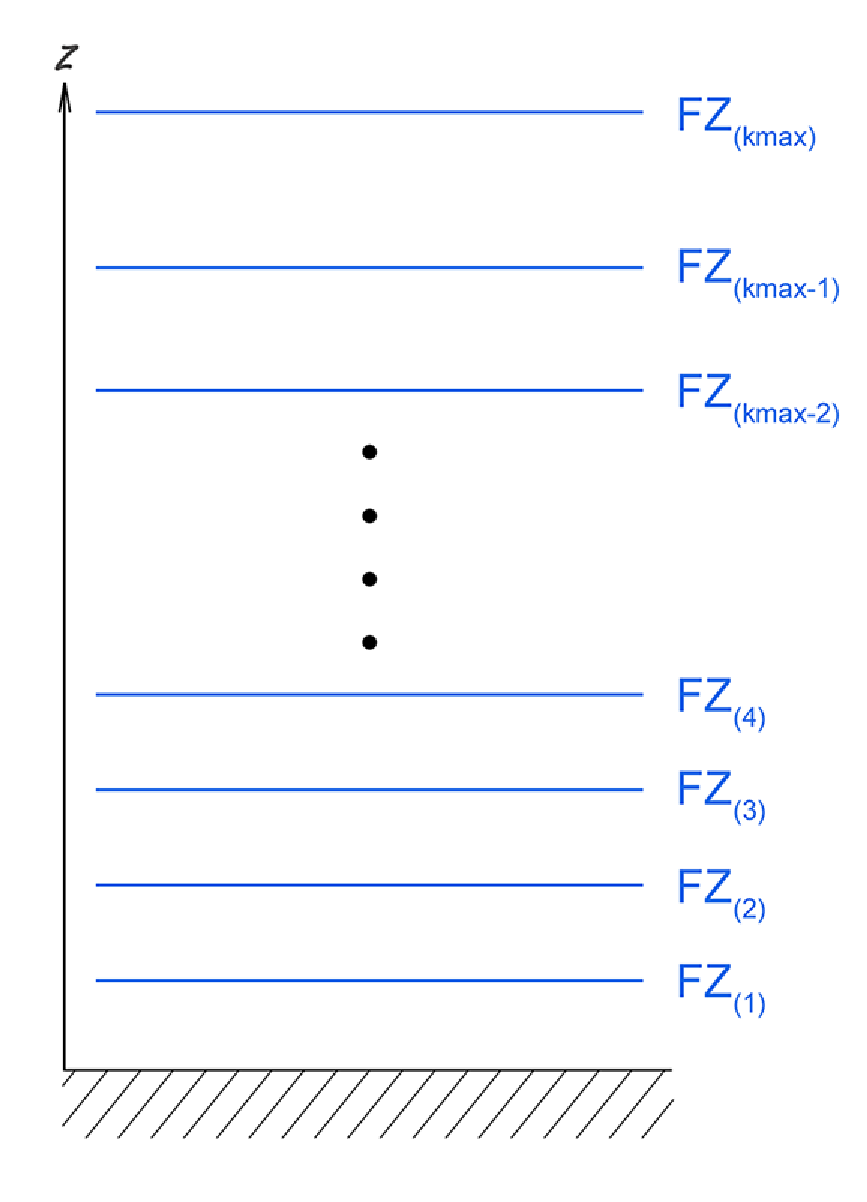
\includegraphics[width=0.4\hsize]{./figure/verticalface.eps}\\
  \caption{\scalerm の鉛直格子の定義点。\namelist{PARAM_GRID}で\nmitem{FZ}を指定する時は、ハロを除いた計算領域下端の格子から$k=1$として与える。}
  \label{fig:scale_grid}
\end{center}
\end{figure}
なお、これらの指定では、
標高0mでの格子点として設定され、標高を持つ位置では山岳に沿った座標系によって適切に処理される。


格子点位置は任意に設定できるが、場合によっては計算不安定につながる。
鉛直層の設定については、作成をサポートするツール(\verb|scale/scale-rm/util/makevgrid/|)が
用意されているので参考にされたい。
\footnote{``make\_vgrid.f90''というFortranプログラムと
いくつかのサンプルnamelistが用意されている。}
ツールをコンパイルして実行すれば直ちに設定ファイルに貼り付けて使用できる
\nmitem{FZ(:)}の値が作成される。

\subsection{\SecBasicBufferSetting} \label{subsec:buffer}
%-----------------------------------------------------------------------
モデル最上層では重力波の反射、
側面境界では現実大気実験/ネスティング実験を行う際に親領域と対象領域の間の不一致が起こる。
この問題を解決するため、「緩和領域」を設ける。
\scalerm では計算領域の境界のすぐ内側に緩和領域を設定することができる。
緩和領域の格子では、指定された値(境界値データ、親領域のデータなど)に対して
ある時定数で緩和される。以下これをナッジングと呼ぶ。
緩和領域の幅は、設定ファイルの\namelist{PARAM_GRID}の中で設定する。
以下に例を示す。
設定はすべての設定ファイルにおいて共通していなければならない。\\

\noindent {\small {\gt
\ovalbox{
\begin{tabularx}{150mm}{lX}
\verb|&PARAM_GRID  |            & \\
 \verb|BUFFER_DZ = 5000.D0,   | & ; {\ZDIR}(モデルトップから下向き方向)の緩和領域の幅 [m]\\
 \verb|BUFFER_DX = 300000.D0, | & ; {\XDIR} (東西方向)の緩和領域の幅 [m]\\
 \verb|BUFFER_DY = 300000.D0, | & ; {\YDIR}(南北方向)の緩和領域の幅 [m]\\
 \verb|BUFFFACT  = 1.D0,      | & ; 緩和領域内の格子間隔に対するストレッチ係数(デフォルトは1.0)\\
\verb|/|\\
\end{tabularx}
}}}\\

水平方向には東西南北の四方境界に緩和領域が設定されるが、
鉛直方向には計算領域の上端にのみ緩和領域が設定され、下端には設定されない。
%
緩和領域は、計算領域内に設定されるため、
ナッジングの影響を受けない領域(緩和領域を除いた範囲)は
計算領域よりも狭くなることに注意が必要である。

\subsubsection{緩和領域の格子間隔をストレッチさせる}
緩和領域の格子間隔は、基本的に 
\namelist{PARAM_GRID}の中の\nmitem{DX, DY, DZ}で指定した通りであるが、
\nmitem{BUFFFACT}に1以上の値を設定することで、ストレッチさせることも可能である。
ただし、格子間隔を等間隔で指定した場合、
この\nmitem{BUFFFACT}の設定は、x, y, {\ZDIR}すべてに適用されることの注意されたい。
{\ZDIR}の層レベルを任意の格子点位置に指定する場合、
すなわち、\nmitem{FZ(:)}を与える場合(第\ref{subsec:gridinterv}節参照のこと)には適用されない。

緩和領域内の格子間隔 (\verb|BDX|) は次の通り決定される。
\begin{eqnarray}
 \verb|BDX(|n\verb|)| &=& \verb|DX| \times \verb|BUFFFACT|^n \nonumber
\end{eqnarray}
ここで、$n$は緩和領域内の格子点番号を表し、計算領域の内側から外側へ向かって番号が振られる。
緩和領域の格子間隔は、
\verb|BUFFFACT=1.0|ならば内部領域と同じであり、
\verb|BUFFFACT=1.2|ならば内側から外側(境界)に向かって1.2倍の割合で広がっていく。
\verb|BUFFFACT|はいくつに設定しても良いが、計算の安定性を考慮すると 1.0から1.2 が推奨である。

緩和領域の格子数\verb|ibuff|は、
\begin{eqnarray}
\sum_{n=1}^{\verb|ibuff|} \verb|BDX|(n) \ge \verb|BUFFER_DX| \nonumber
\end{eqnarray}
の関係を満たす最小の整数で自動的に計算される。
%
緩和領域の幅(\nmitem{BUFFER_DX})が同じでも、
\nmitem{BUFFFACT}の値を大きくすると緩和領域に用意される格子数は少なくなる。
ここでは、{\XDIR} の説明をしたが、{\YDIR}、{\ZDIR}も同様である。


一般に、緩和領域の大きさ、緩和格子点の数については、解く問題により、明確な指標はない。
\scalerm では、鉛直方向(計算領域トップ)の緩和格子点は5点以上、
水平方向(側面境界付近)の緩和格子点は20〜40点程度を推奨している。
実験設定や事例によっては、さらに緩和格子点を増やしたり、
ストレッチ係数を用いて緩和領域を広げたり、
ここでは説明しないが
\namelist{PARAM_ATMOS_BOUNDARY}の中の
\nmitem{ATMOS_BOUNDARY_taux,ATMOS_BOUNDARY_tauy}を調整して
緩和領域のナッジング強度を調整したりする必要があるだろう。


\subsection{\SecBasicTopoSetting} \label{subsec:basic_usel_topo}
%-----------------------------------------------------------------------

\scalerm では地形データに対しモデル下端の格子面を傾斜させて地形を表現するTerrain followingを採用している。
力学計算過程において安定的に計算を実行するためには、この地形の傾斜角度が45度以下でなければならない。
水平の最大格子間隔をDX [m]、鉛直の最小格子間隔をDZ [m]とすると、地形傾斜角度$\theta$[deg]は次の式で計算される。

\[ \theta = \arctan( DZ/DX ) * 180/pi \]

地形の設定は、設定ファイルの\namelist{PARAM_CNVTOPO}の中で設定する。
以下に例を示す。\\

\noindent {\small {\gt
\ovalbox{
\begin{tabularx}{150mm}{lX}
\verb|&PARAM_CNVTOPO  |            & \\
 \verb|CNVTOPO_name            = "GTOPO30", | & ; 使用する地形データ名\\
 \verb|CNVTOPO_smooth_maxslope = 0.229,     | & ; 許容する最大傾斜角度 [deg]\\
 \verb|CNVTOPO_smooth_local    = .true.,    | & ; 傾斜を緩める範囲を最大傾斜角度を超えた格子のみ行うかどうか \\
 \verb|CNVTOPO_smooth_itelim   = 10000,     | & ; 傾斜を緩める際の反復計算回数 \\
 \verb|CNVTOPO_copyparent      = .false.,   | & ; 緩和領域に親ドメインの地形データのコピーするかどうか \\
\verb|/|\\
\end{tabularx}
}}}\\

使用する地形データの名称を与え、地形データを読み込む。
\scalerm ではGTOPO30、または国土地理院による高精度地形データ(DEM50M)をサポートしている。

設定された地形傾斜角度を超える傾斜が与えられた地形データ内に検出された場合、
それを設定された地形傾斜角度以下になるように、反復計算を用いて徐々に傾斜を緩めていく。
このとき、傾斜を緩める範囲を最大傾斜角度を超えた格子のみ行うか、計算領域全体で行うかを選択することができる。
前者は、最大傾斜角度以内のシャープな地形構造を残すことができるので、細かな地形表現を望む場合に選択する。
最大傾斜角度が小さい場合、反復計算回数が相当に大きな数になる場合があるので、適宜反復計算の最大回数を調整する。

上記の計算式で分かるように、許容される最大傾斜角度は空間解像度に応じて変わる。
一般的に、多段ネスティング計算を行う場合、
子ドメインのほうが空間解像度が細かいため、地形もシャープに表現される。
このとき、親ドメインと子ドメインの地形表現が異なるために、
子ドメインの緩和領域に挿入される親ドメインの大気データを外挿する必要が発生し、不整合を起こすことがある。
これを回避するために、
\nmitem{CNVTOPO_copyparent}を\verb|.true.|とすることで、親ドメインの地形データを子ドメインの緩和領域にコピーすることができる。
親ドメインが存在しない場合は\nmitem{CNVTOPO_copyparent}を必ず\verb|.false.|に設定しなければならない。

\newpage
\section{積分時間と積分時間間隔の設定} \label{sec:timeintiv}
%------------------------------------------------------
積分時間やタイムステップは、実験の目的や設定によって適切に設定する必要がある。
空間解像度を変えた場合はそれに応じたタイムステップを設定する必要があり、
同じ解像度でも計算不安定を防ぐためにタイムステップを短くすることもある。

積分時間とタイムステップの設定は、
設定ファイル\verb|run_***.conf|の\verb|PARAM_PRC|の項目を編集することで設定できる。
この項目はモデル本体(\verb|scale-rm|)実行時のみで有効であり、初期化作成時には無効である。\\

\noindent {\small {\gt
\ovalbox{
\begin{tabularx}{140mm}{lX}
\verb|&PARAM_TIME| & \\
\verb| TIME_STARTDATE             = 2014, 8, 10, 0, 0, 0,| & 計算開始の日付:放射過程を用いる実験等で必要\\
\verb| TIME_STARTMS               = 0.D0,  | & 計算開始時刻[mili sec]\\
\verb| TIME_DURATION              = 12.0D0,| & 積分時間[単位は\verb|TIME_DURATION_UNIT|で設定]\\
\verb| TIME_DURATION_UNIT         = "HOUR",| & \verb|TIME_DURATION|の単位\\
\verb| TIME_DT                    = 60.0D0,| & トレーサー移流のタイムステップ\\
\verb| TIME_DT_UNIT               = "SEC", | & \verb|TIME_DT|の単位 \\
\verb| TIME_DT_ATMOS_DYN          = 30.0D0,| & 力学過程計算のタイムステップ\\
\verb| TIME_DT_ATMOS_DYN_UNIT     = "SEC", | & \verb|TIME_DT_ATMOS_DYN|の単位\\
\verb| TIME_DT_ATMOS_PHY_MP       = 60.0D0,| & 雲物理過程のタイムステップ \\
\verb| TIME_DT_ATMOS_PHY_MP_UNIT  = "SEC", | & \verb|TIME_DT_ATMOS_PHY_MP|の単位\\
\verb| TIME_DT_ATMOS_PHY_TB       = 60.0D0,| & 乱流スキームのタイムステップ \\
\verb| TIME_DT_ATMOS_PHY_TB_UNIT  = "SEC", | & \verb|TIME_DT_ATMOS_PHY_TB|の単位\\
\verb| TIME_DT_ATMOS_PHY_RD       = 600.0D0, | & 放射スキームのタイムステップ \\
\verb| TIME_DT_ATMOS_PHY_RD_UNIT  = "SEC",  | & \verb|TIME_DT_ATMOS_PHY_RD|の単位\\
\verb| TIME_DT_ATMOS_PHY_SF       = 60.0D0, | & 大気下端境界(フラックス計算)のタイムステップ\\
\verb| TIME_DT_ATMOS_PHY_SF_UNIT  = "SEC",  | & \verb|TIME_DT_ATMOS_PHY_SF|の単位\\
\verb| TIME_DT_OCEAN              = 300.0D0,| & 海面・海洋スキームのタイムステップ\\
\verb| TIME_DT_OCEAN_UNIT         = "SEC",  | & \verb|TIME_DT_OCEAN|の単位\\
\verb| TIME_DT_LAND               = 300.0D0,| & 陸面スキームのタイムステップ\\
\verb| TIME_DT_LAND_UNIT          = "SEC",  | & \verb|TIME_DT_LAND|の単位\\
\verb| TIME_DT_URBAN              = 300.0D0,| & 都市スキームのタイムステップ\\
\verb| TIME_DT_URBAN_UNIT         = "SEC",  | & \verb|TIME_DT_URBAN|の単位\\
\verb| TIME_DT_ATMOS_RESTART      = 21600.D0, | & リスタートファイル(大気)の出力間隔\\
\verb| TIME_DT_ATMOS_RESTART_UNIT = "SEC",    | & \verb|TIME_DT_ATMOS_RESTART|の単位\\
\verb| TIME_DT_OCEAN_RESTART      = 21600.D0, | & リスタートファイル(海洋)の出力間隔\\
\verb| TIME_DT_OCEAN_RESTART_UNIT = "SEC",    | & \verb|TIME_DT_OCEAN_RESTART|の単位\\
\verb| TIME_DT_LAND_RESTART       = 21600.D0, | & リスタートファイル(陸面)の出力間隔\\
\verb| TIME_DT_LAND_RESTART_UNIT  = "SEC",    | & \verb|TIME_DT_LAND_RESTART|の単位\\
\verb| TIME_DT_URBAN_RESTART      = 21600.D0, | & リスタートファイル(都市)の出力間隔\\
\verb| TIME_DT_URBAN_RESTART_UNIT = "SEC",    | & \verb|TIME_DT_URBAN_RESTART|の単位\\
\verb|/|\\
\end{tabularx}
}}}\\


\verb|TIME_DT| は、トレーサー移流のためのタイムステップであり、
格子間隔と移流速度からクーラン条件(CFL条件)を満たすように決定する。
つまり、格子間隔を移流速度で割った値が取りうる最少値よりも小さな値を設定する。
\verb|TIME_DT_ATMOS_DYN| は、力学変数の時間積分のためのタイムステップであり、音速で制約される。
計算安定性のためには、\verb|ATMOS_DYN_TINTEG_SHORT_TYPE| が \verb|RK4| の場合には
最少格子間隔(HE-VI利用時には水平の最少格子間隔)を 420 m/s で割った値が、
\verb|RK3| の場合には 840 m/s で割った値が目安となる。




\input{56_basic_historysetting}
\input{57_basic_dynsetting}
\input{58_basic_physsetting}

\chapter{各種設定: 実用編} \label{chap:advance_use}
\section{概要} \label{sec:advance_use_overview}

この章では、更に発展的な使い方似ついて説明する。
以下に、項目を列挙する。

{
\begin{center}
\begin{tabular}[h]{ll}\hline
\SecAdvanceMapprojectionSetting & 第\ref{sec:adv_mapproj}節 \\
\SecAdvanceInputDataSetting & 第\ref{sec:adv_datainput}節\\
\SecAdvanceRestart & 第\ref{sec:restart}節 \\
\SecAdvancePostprosess & 第\ref{sec:net2g}節 \\
\SecAdvanceNesting & 第\ref{sec:nest_exp}節 \\
\SubsecOflineNesting & 第\ref{subsec:nest_offline}節\\
\SubsecOnlineNesting & 第\ref{subsec:nest_online}節\\
\SecAdvanceBulkjob & 第\ref{sec:bulkjob}節\\
\hline
\end{tabular}
\end{center}
}




\section{地図投影法と計算領域の位置} \label{sec:adv_mapproj}
%------------------------------------------------------
計算領域の位置と投影法は、設定ファイルの\verb|PARAM_MAPPROJ|の項目を編集することで設定できる。
\textcolor{red}{\bf この設定も、pp\_***.conf、init\_***.conf、run\_***.confの設定ファイルの間で
必ず一致させなければならない。}はじめに下記の例をもとに説明する。\\

\noindent {\small {\gt
\ovalbox{
\begin{tabularx}{140mm}{l}
\verb|&PARAM_MAPPROJ| \\
\verb| MPRJ_basepoint_lon = 138.727778D0,| \\
\verb| MPRJ_basepoint_lat = 35.360556D0,| \\
\verb| MPRJ_type          = 'MER',| \\
\verb|/| \\
\end{tabularx}
}}}\\

\noindent まず\verb|MPRJ_basepoint_lat|と\verb|MPRJ_basepoint_lon|は、計算領域の中心の緯度・経度を表す。
SCALEでは、北緯を正、南緯を負の値として表現し、経度は0度を起点に右回りで表現するため、この設定では計算領域の
中心が北緯35.360556度、東経138.727778度に位置することになる。この場所を中心に指定された大きさで、計算領域が
設定される\footnote{デフォルトではメルカトル図法に基づいて緯度・経度を計算する際の基準とする緯度は、
MPRJ\_basepoint\_latの値が使用されるが、MPRJ\_M\_latを用いて任意の緯度を指定することもできる。}。
実際にはSCALE内部での格子点は実距離に基づいて格子点が配置されるので、投影法で設定されるのは、
実距離に基づいた緯度・経度座標が計算される。この緯度・経度情報は、すべてのSCALEのNetCDF形式の出力ファイルに
含まれている。

\verb|MPRJ_type|は、地図投影法の種類を表しており、\verb|MER|はメルカトル図法を意味する。
SCALEで現在選択できる地図投影法とその指定文字列は次のとおりである。

\begin{table}[htb]
\begin{center}
\caption{SCALEで選択できる地図投影法}
\begin{tabularx}{150mm}{|l|X|} \hline
 \rowcolor[gray]{0.9} 地図投影法 & \verb|MPRJ_type| \\ \hline
 地図投影なし(理想実験用)& \verb|NONE| \\ \hline
 ランベルト正角円錐図法 & \verb|LC| \\ \hline
 極心平射図法(ポーラーステレオ) & \verb|PS| \\ \hline
 メルカトル図法 & \verb|MER| \\ \hline
 正距円筒図法 & \verb|EC| \\ \hline
\end{tabularx}
\label{tab:map_proj}
\end{center}
\end{table}

メルカトル図法以外の投影法も、\verb|MPRJ_type|の指定を変更するだけで、上記と同じように使用可能であるが、
ランベルト正角円錐図法の設定方法については、設定方法が異なるため以下で説明する。ここでは、現実大気実験
チュートリアルで使用した\verb|run.conf|ファイルを例に挙げる。\\

\noindent {\small {\gt
\ovalbox{
\begin{tabularx}{140mm}{l}
\verb|&PARAM_MAPPROJ| \\
\verb| MPRJ_basepoint_lon = 135.220404D0,| \\
\verb| MPRJ_basepoint_lat = 34.653396D0,| \\
\verb| MPRJ_type          = 'LC',| \\
\verb| MPRJ_LC_lat1       =  30.00D0,| \\
\verb| MPRJ_LC_lat2       =  40.00D0,| \\
\verb|/| \\
\end{tabularx}
}}}\\

SCALEでは``standard parallel type''の実装を採用しているため、投影を決定する上で2つの``standard latitude''の
位置を指定する必要がある。2つのstandard latitudeに挟まれた領域では、緯線・経線の長さの比が地球楕円体面上における
長さの比と近くなるように調節される。従って、メルカトル図法の場合に比べて、standard latitudeを設定する
\verb|MPRJ_LC_lat1|と\verb|MPRJ_LC_lat2|の項目が追加されている。それぞれ、南側、北側のstandard latitudeの
値を``degree''で指定する。

さらに下記のように\verb|MPRJ_basepoint_x|と\verb|MPRJ_basepoint_y|という変数を用いることで、地図投影中心と
計算領域中心をずらすこともできる。\\

\noindent {\small {\gt
\ovalbox{
\begin{tabularx}{140mm}{l}
\verb|&PARAM_MAPPROJ| \\
\verb| MPRJ_basepoint_lon = 135.220404D0,| \\
\verb| MPRJ_basepoint_lat = 34.653396D0,| \\
\verb| MPRJ_basepoint_x   = 100.0D0,| \\
\verb| MPRJ_basepoint_y   = 100.0D0,| \\
\verb| MPRJ_type          = 'LC',| \\
\verb| MPRJ_LC_lat1       =  30.00D0,| \\
\verb| MPRJ_LC_lat2       =  40.00D0,| \\
\verb|/| \\
\end{tabularx}
}}}\\

\noindent \verb|MPRJ_basepoint_x|と\verb|MPRJ_basepoint_y|は、地図投影中心の位置を、計算領域の南西端(左下角)から
の距離で指定するパラメータで、単位はメートルである。これらを指定しない場合は、デフォルト設定として計算領域中心と
地図投影中心の位置は一致する。上記の場合とデフォルト設定の場合を比較したものが図\ref{fig:map_lc}である。
図\ref{fig:map_lc}aはデフォルト設定で投影中心と計算領域中心が一致している場合、図\ref{fig:map_lc}bは、
計算領域の位置を投影中心からずらした場合の関係を表している。図\ref{fig:map_lc}bでは、計算領域の南西端から
\verb|MPRJ_basepoint_x|と\verb|MPRJ_basepoint_y|で指定した距離だけ離れた位置に投影中心がある。

\begin{figure}[t]
\begin{center}
  \includegraphics[width=0.8\hsize]{./figure/LC_latlon_xy.eps}\\
  \caption{投影中心と計算領域の関係:(a)はデフォルト設定の場合、(b)は計算領域の位置を投影中心からずらした場合。
  赤線の矩形が計算領域を表す。}
  \label{fig:map_lc}
\end{center}
\end{figure}


\input{63_advance_howtoinput}
\section{\SecAdvanceRestart}\label{sec:restart}
%=======================================================================

\section{Postprocess : net2g} \label{sec:net2g}
%====================================================================================

本節では、SCALEの後処理ツールnet2gについて説明する。net2gは、SCALE-RMで出力された
領域分割のnetcdf形式historyデータ(\verb|history.***.nc|)を結合しGrADSで読み込める
バイナリ形式に変換するツールである。
分割データを結合することで、GrADSでの描画に適するだけでなく、Fortranプログラムなどで
解析しやすいデータになる。
net2gはMPI並列実行も可能であり、単一プロセス実行に比べて変換に要する時間を短縮できる。
その他、net2gの機能として次のものが利用できる。

\begin{itemize}
 \item モデル面から任意の鉛直高度座標、鉛直気圧座標への内挿
 \item 3次元変数に対する鉛直の積算値、平均値、最大値、最小値の出力
 \item 3次元変数を鉛直層ごとに分割したファイルとしての出力
 \item 時間ステップごとに分割したファイルとしての出力
\end{itemize}

特に大規模計算結果においては、鉛直層や時間ステップごとに分割することで
ハンドリングしやすいデータサイズにして保存することができるため便利である。
さらに、大規模計算結果を解析するだけのケースを踏まえてポータビリティを重視した設計とし、
SCALEライブラリに対する依存性をなくしたため、net2gだけを独立にコンパイル・実行できることも特徴である。
net2gのインストール方法については、\ref{sec:source_net2g}節を参照すること。

ただし、現行のnet2gにおいては下記の制約がある。
\begin{itemize}
 \item net2gに使用するMPIプロセス数は、SCALE-RM実行時に使用したMPIプロセス数の約数でなければならない。
 \item SCALE-RM実行時のhistory出力形式は、``\verb|HIST_BND = .false.|''でなければならない。
 \item 2次元データと3次元データは同時に変換できない。
 \item 変換できるデータはhistoryデータのみである。
\end{itemize}
\noindent これらの制約を無くすため、今後早急に対応を進める予定である。

その他に注意するべき点は、net2g実行時のMPIプロセス数をむやみに大きくしないことである。
net2gは実行内容のほとんどがデータ入出力であるため、MPIプロセス数を増やしすぎると
読み込み/書き込み要求が立て込んで、作業効率が下がり、結果として実行速度が落ちることもある。
特に大規模計算結果を手元のマシンで変換する際は注意が必要である。

net2gの実行はMPI並列を用いて、
\begin{verbatim}
 $ mpirun  -n  [procs]  ./net2g  net2g.conf
\end{verbatim}
とする。\verb|[procs]|には任意のMPIプロセス数を指定する。最後の``net2g.conf''はnet2gの実行設定が
記述された設定ファイルである。一方、シングルプロセス版としてコンパイルした場合はMPIコマンドを使わずに、
\begin{verbatim}
 $ ./net2g  net2g.conf
\end{verbatim}
とする。
エラーメッセージがなく、次のメッセージだけが標準出力へ表示されて終了すれば変換完了である。\\

\noindent {\gt
\fbox{
\begin{tabularx}{140mm}{l}
\verb|+++ MPI COMM: Corrective Finalize| \\
\end{tabularx}
}}\\

次に、3次元変数と2次元変数を変換する場合における設定ファイルの記述方法について説明する。
それぞれ、``scale/scale-rm/util/netcdf2grads\_h/''のディレクトリに
入っている``net2g.3d.conf''と``net2g.2d.conf''に基づいて説明する。
本節では主要な設定項目だけを取り上げる。
ここで触れなかったオプションについては、``scale/scale-rm/util/netcdf2grads\_h/''のディレクトリに
入っている設定ファイルサンプル``net2g.all.conf''を参照してもらいたい。


\subsubsection{設定ファイルサンプル:3次元変数の変換}
%------------------------------------------------------

\noindent {\small {\gt
\ovalbox{
\begin{tabularx}{140mm}{l}
\verb|&LOGOUT| \\
\verb| LOG_BASENAME   = "LOG_d01_3d",| \\
\verb| LOG_ALL_OUTPUT = .false.,| \\
\verb|/| \\
 \\
\verb|&INFO| \\
\verb| START_TSTEP = 1,| \\
\verb| END_TSTEP   = 25,| \\
\verb| DOMAIN_NUM  = 1,| \\
\verb| CONFFILE    = "../run/run.d01.conf",| \\
\verb| IDIR        = "../run",| \\
\verb| Z_LEV_TYPE  = "plev",| \\
\verb|/| \\
 \\
\verb|&VARI| \\
\verb| VNAME       = "PT","U","V","W","QHYD",| \\
\verb| TARGET_ZLEV = 850,500,200,| \\
\verb|/| \\
\end{tabularx}
}}}\\

\noindent 上記はあるdomainの3次元変数を、気圧高度面へ内挿して出力する場合の
例を示している。各々の設定項目は次のとおりである。
\begin{itemize}
 \item \namelist{LOGOUT}(このNamelistは必須ではない)
 \begin{itemize}
  \item \verb|LOG_BASENAME|:デフォルトのLOGファイル名``LOG''を変更したいときに指定する。
  \item \verb|LOG_ALL_OUTPUT|:プロセス番号0番以外もLOGファイルを出力させたい場合に``true''にする。
        デフォルト値は``false''である。
 \end{itemize}
 \item \namelist{INFO}
 \begin{itemize}
  \item \verb|START_TSTEP|:変換するNetCDFデータの最初のTime Stepを指定する。最初のいくつかの
        ステップを飛ばして変換したい場合に任意の値を指定する。デフォルト値は1である。
  \item \verb|END_TSTEP|:変換するNetCDFデータの最後のTime Stepを指定する。必ず指定すること。
  \item \verb|DOMAIN_NUM|:ドメイン番号を指定する。デフォルト値は1である。
  \item \verb|CONFFILE|:SCALE-RM本体を実行したときの\verb|run.***.conf|ファイルのPATHを指定する
        (ファイル名を含む)。
  \item \verb|IDIR|:SCALE-RM本体のhistory出力ファイルのPATHを指定する。
  \item \verb|Z_LEV_TYPE|:鉛直方向のデータ変換の種類を指定する。``original''はモデル面、
        ``plev''は気圧面に内挿、そして``zlev''は高度面に内挿して出力する。
        ``anal''を指定すると別途指定の簡易解析を行なって出力する(次項で説明)。デフォルト値は``plev''である。
 \end{itemize}
 \item \namelist{VARI}
 \begin{itemize}
  \item \verb|VNAME|:変換したい変数名を指定する。デフォルトでは、``PT''、``PRES''、``U''、``V''、
        ``W''、``QHYD''が指定される。
  \item \verb|TARGET_ZLEV|:\verb|Z_LEV_TYPE|に応じた変換高度を指定する。plevの場合は``hPa''、
        zlevの場合は``m''、そしてoriginalの場合は格子点番号で指定する。デフォルトでは、
        1000hPa、975hPa、950hPa、925hPa、900hPa、850hPa、800hPa、700hPa、600hPa、500hPa、400hPa、
        300hPa、250hPa、200hPaの14層が指定される。 
 \end{itemize}
\end{itemize}

\subsubsection{設定ファイル変更例:3次元変数の変換:鉛直積算値を出す}
%------------------------------------------------------

\noindent {\small {\gt
\ovalbox{
\begin{tabularx}{140mm}{l}
\verb|&INFO| \\
\verb|    〜 中略 〜|\\
\verb| Z_LEV_TYPE  = "anal",| \\
\verb| ZCOUNT      = 1,| \\
\verb|/| \\
 \\
\verb|&ANAL| \\
\verb| ANALYSIS    = "sum",| \\
\verb|/| \\
 \\
\verb|&VARI| \\
\verb| VNAME       = "QC","QI","QG",| \\
\verb|/| \\
\end{tabularx}
}}}\\

\noindent 上記は、簡易解析を利用する場合の設定ファイル変更例の抜粋である。
他の設定項目については先の3次元変数の変換の場合と同じである。
\verb|Z_LEV_TYPE|を``anal''と指定することで、3次元変数の鉛直次元に対する簡易解析が有効になり、
\namelist{ANAL}を指定できるようになる。
このとき変換後のデータは必ず水平2次元データとなるため、\namelist{VARI}の\nmitem{TARGET_ZLEV}は
指定できない。
また、2次元データ出力を指定するため、\textcolor{red}{\namelist{INFO}の\nmitem{ZCOUNT}を必ず``1''と指定する。}

\begin{itemize}
 \item \namelist{ANAL}
 \begin{itemize}
  \item \verb|ANALYSIS|:鉛直次元のの簡易解析の種類を指定する。``max''を指定すると鉛直カラム中の最大値、
        ``min''を指定するすると最小値、``sum''を指定すると鉛直カラム積算値、そして``ave''を指定すると
        鉛直カラム平均値を算出する。デフォルト値は``ave''である。現時点では、単純な積算値や平均値の出力であり、
        混合比に密度を掛けて質量にして出力する等の機能は有していない。
 \end{itemize}
\end{itemize}

\subsubsection{設定ファイルサンプル:2次元変数の変換}
%------------------------------------------------------

\noindent {\small {\gt
\ovalbox{
\begin{tabularx}{140mm}{l}
\verb|&LOGOUT| \\
\verb| LOG_BASENAME   = "LOG_d01_2d",| \\
\verb|/| \\
 \\
\verb|&INFO| \\
\verb| START_TSTEP = 1,| \\
\verb| END_TSTEP   = 25,| \\
\verb| DOMAIN_NUM  = 1,| \\
\verb| CONFFILE    = "../run/run.d01.conf",| \\
\verb| IDIR        = "../run",| \\
\verb| ZCOUNT      = 1,| \\
\verb|/| \\
 \\
\verb|&VARI| \\
\verb| VNAME       = "T2","MSLP","PREC"| \\
\verb|/| \\
\end{tabularx}
}}}\\

\noindent 上記はあるdomainの2次元変数をデータ形式変換する場合の設定例である。
\textcolor{red}{2次元変数の変換を指定するため、\namelist{INFO}の\nmitem{ZCOUNT}を必ず``1''と指定する。}
また、2次元データなので\namelist{VARI}の
\nmitem{TARGET_ZLEV}は指定できない。その他の設定項目は3次元変数変換の場合と変わりない。


\subsubsection{設定ファイル変更例:特殊な時間軸を持つデータの変換}
%------------------------------------------------------

\noindent {\small {\gt
\ovalbox{
\begin{tabularx}{140mm}{l}
\verb|&EXTRA| \\
\verb| EXTRA_TINTERVAL = 600.0,| \\
\verb| EXTRA_TUNIT     = "SEC",| \\
\verb|/| \\
 \\
\verb|&VARI| \\
\verb| VNAME = "RAIN",| \\
\verb|/| \\
\end{tabularx}
}}}\\

\noindent 上記は設定ファイル変更例である。その他の項目は先の3次元や2次元変数の場合と同じである。
SCALE-RM実行時に、\ref{sec:output}節の最後で説明した出力アイテム毎の設定で、\namelist{HISTITEM}の
\nmitem{TINTERVAL}を設定し、一部の出力変数が\nmitem{HISTORY_DEFAULT_TINTERVAL}に
従わない場合、net2gでは\namelist{EXTRA}を上記のように設定することで対応できる。
この例では、\ref{sec:output}節の最後で説明した設定に合わせて、2次元データの``RAIN''だけが
600秒間隔で出力された場合の例を示している。
net2gでは、異なる出力時間間隔を同時に取り扱うことはできないため、
複数の異なる出力間隔が存在するhistoryデータにおいては、それぞれに独立してnet2gを走らせる必要がある。


\subsection{大型並列計算機での実行} \label{subsec:on_supercom}
%------------------------------------------------------

スーパーコンピュータ「京」などの大型計算機で大規模並列計算を行った場合、出力ファイルの数が多く、
それぞれのファイルのデータ容量も大きい。そのような場合には、手元のマシンへhistoryデータをコピーするだけの
ディスク容量がなかったり、後処理に膨大な時間がかかることがある。
こういった場合には、SCALE-RM本体の計算を行ったスーパーコンピュータ上で後処理も行なってしまうことを
おすすめする。

スーパーコンピュータ「京」では、\ref{subsec:set_evniromnet}節で説明されている環境変数の設定がされていれば、
net2gはそのままmakeコマンドでコンパイルできる。

ジョブの投入・実行方法については、スーパーコンピュータ「京」のユーザーズマニュアル等を参照されたい。
net2gの実行方法や制約、注意点については通常のマシンで実行する場合と何ら変わりない。

%% サポート外
%%
%% \noindent {\gt \verb|job.sh|の記述例} \\
%% \noindent {\small {\gt
%% \ovalbox{
%% \begin{tabularx}{140mm}{l}
%% \verb|#! /bin/bash -x| \\
%% \verb|#PJM --rsc-list "rscgrp=micro"| \\
%% \verb|#PJM --rsc-list "node=12"| \\
%% \verb|#PJM --rsc-list "elapse=00:30:00"| \\
%% \verb|#PJM -j| \\
%% \verb|#PJM -s| \\
%% \verb|#| \\
%% \verb|. /work/system/Env_base| \\
%% \verb|#| \\
%% \verb|export PARALLEL=8| \\
%% \verb|export OMP_NUM_THREADS=8| \\
%% \verb|#| \\
%% \verb|mpiexec -n 12 ./net2g  n2g_d01-3d.conf| \\
%% \end{tabularx}
%% }}}\\


%% サポート外(今後、統合サポート予定)
%%
%% \subsection{バルクジョブ対応版の使用方法}
%% %------------------------------------------------------

%% \ref{sec:bulkjob}節で説明した「複数の実験を一括実行するバルクジョブ機能」を用いてSCALEを走らせた場合は、
%% バルクジョブ対応版のnet2gを利用するのが便利である。コンパイルは、通常版のnet2gと同じである。
%% ``scale/scale-rm/util/netcdf2grads\_bulk''の下で\ref{sec:source_net2g}節で説明したとおりの方法で
%% コンパイルすれば、バルクジョブ対応版のnet2gが生成される。

%% 基本的な使用方法や制限事項も通常版のnet2gと同じである。net2gに渡す設定ファイルなどの記述も通常版と
%% 同じように記述すればよい。ただし、実行にあたっては``launch.conf''が必要になることと、\ref{sec:bulkjob}節で
%% 説明したバルクジョブ実行時のディレクトリ構造を準備する必要がある。SCALE本体をバルクジョブ機能で実行した
%% 場合にはディレクトリ構造はすでに準備されているため新たに用意する必要はない。net2gに渡す設定ファイルだけ、
%% 各バルク番号のディレクトリ下に設置すればよい。以下に、launch.confファイルの記述例を挙げておく。\\

%% \noindent {\small {\gt
%% \ovalbox{
%% \begin{tabularx}{140mm}{l}
%% \verb|&PARAM_LAUNCHER| \\
%% \verb| NUM_BULKJOB = 31,| \\
%% \verb| NUM_DOMAIN  = 2,| \\
%% \verb| PRC_DOMAINS = 12,36,| \\
%% \verb| CONF_FILES  = net2g.3d.d01.conf,net2g.3d.d02.conf,| \\
%% \verb|/| \\
%% \end{tabularx}
%% }}}\\

%% \noindent この例の場合、一度に31個のジョブを実行している。また1つのジョブは2段オンライン・ネスティング実験
%% となっており、net2gの実行にあたってはdomain 1は12-MPI並列、domain 2は36-MPI並列で実行される。ここで
%% 指定するMPIプロセス数は、SCALE本体の実行時に使用したMPIプロセス数の約数でなければならない。

%% それぞれのドメインについて実行するnet2gの設定ファイルは、
%% それぞれ``net2g.3d.d01.conf''と``net2g.3d.d02.conf''と指定されている。
%% この設定ファイルは31個のバルク番号ディレクトリの中に
%% 収められてことを想定している。

%% この例では、1つのジョブあたり、$12 + 36 = 48$プロセスを使用し、全体で31ジョブあるので総計で1488プロセスを
%% 必要とする。下記のコマンドのように実行する。

%% \begin{verbatim}
%%  $ mpirun  -n  1488  ./net2g  launch.conf
%% \end{verbatim}


%% サポート外
%%
%% \subsection{旧型netcdf2gradsの使用方法}
%% %------------------------------------------------------
%% ここでは、シングルプロセス実行しかできないが、``HIST\_BND''の対応、そしてhistoryデータ以外のデータにも対応
%% する「旧型netcdf2grads」の実行方法概略について説明する。このプログラムは、並列版/シングル版net2gの整備が
%% 済み次第、サポート外となるため注意して欲しい。

%% netcdf2gradsのソースファイルは \verb|scale/scale-rm/util/netcdf2grads/|にある。
%% SCALE本体とは独立なので、ディレクトリを任意の場所に移動/コピーして使用することが可能である。

%% \subsubsection{コンパイル}
%% \begin{description}
%% \item[Intel compiler]\mbox{}\\
%%  \begin{verbatim}
%%  $ ifort -convert big_endian -assume byterecl -I${NETCDF4}/include 
%%     -L${NETCDF4}/lib -lnetcdff -lnetcdf make_grads_file.f90 -o convine
%%   \end{verbatim}
%% \item[gfortran]\mbox{}\\
%% \begin{verbatim}
%%  $ gfortran -frecord-marker=4 --convert=big-endian -I${NETCDF4}/include
%%     -L${NETCDF4}/lib -lnetcdff -lnetcdf make_grads_file1.f90 -o convine
%% \end{verbatim}
%% \end{description}

%% \subsubsection{使用方法}
%% 実行時に,インタラクティブモードかサイレントモードかを選択することが出来る.
%% \begin{verbatim}
%%    Interactive mode :  ``./convine -i''
%%    Silent mode      :  ``./convine -s''
%% \end{verbatim}
%% \begin{description}
%% \item[インタラクティブモード]\mbox{}\\
%% \begin{verbatim}
%%  $ cd netcdf2grads/
%%  $ ./convine -i
%% \end{verbatim}
%% と実行すると、下記のメッセージが出るので、指示通りに必要なファイルのパスを打ち込む。\\

%% \noindent {\small {\gt
%% \fbox{
%% \begin{tabularx}{140mm}{l}
%% \verb|path to configure file for run with the quotation mark| \\
%% \textcolor{blue}{\verb| `${path to directory of configure file}/run.conf' <- configureファイルへのパス|} \\
%% \verb|path to directory of history files with the quotation mark| \\
%% \textcolor{blue}{\verb| `${path to directory of history files}/' <- SCALE-RMの出力ファイルのパス|} \\
%% \verb|path to directory of output files with the quotation mark| \\
%% \textcolor{blue}{\verb| `./grads/'  <- gradsファイルの出力先|} \\
%% \verb|start time of convert data| \\
%% \textcolor{blue}{\verb| 1           <- 任意の番号の時間から変換可能 |} \\
%% \verb|end time of convert data| \\
%% \textcolor{blue}{\verb| 10          <- 変換を終了する時間|} \\
%% \verb|Imput number of variable| \\
%% \verb|0 -> all variable output from model| \\
%% \textcolor{blue}{\verb| X           <- 変換したい変数の数|} \\
%% \verb|Imput variable| \\
%% \textcolor{blue}{\verb| VARIABLE(PRECなど)  <- 変換したい変数名|} \\
%% \end{tabularx}
%% }}}\\

%% \noindent \textcolor{blue}{青色文字}の行は、ユーザーが入力する行である。
%% うまく実行されれば、指定した出力先にctlファイルとgrdファイルが作成される。
%% \item[サイレントモード]\mbox{}\\
%% サイレントモードの場合は、あらかじめ、\verb|namelist.in|に必要な情報を書き入れておく.
%% \begin{verbatim}
%%  $ cd netcdf2grads/
%%  $ ./convine -s
%% \end{verbatim}
%% と実行すれば変換が始まる。
%% \end{description}


%####################################################################################


\section{領域ネスティング実験} \label{sec:nest_exp}
%====================================================================================

本節では、SCALEでネスティング実験を行う方法について説明する。ネスティング実験とは、図\ref{fig_nestsample}に
示すように、水平格子間隔の異なる複数の計算領域(ドメイン)を設定し、領域が重複するように入れ子(ネスト)構造に
することで、広領域かつ高解像度の領域を設定する計算領域設定方法である。図\ref{fig_nestsample}の例では、
3つの領域を用いた3段ネスティング構成になっている。外側の領域は比較的粗い
水平解像度であるが広い領域を取ることで大きな場の構造を表現することができる。逆に内側の領域は、比較的狭い
領域であるが細かい水平解像度を取ることで対象とする現象の細かい構造を表現することができる。ここでは、
入れ子構造のうち、データを渡す側の領域を「親領域」、データを受ける側の領域を「子領域」と称する。

SCALEはオフライン・ネスティング実験とオンライン・ネスティング実験の両方をサポートしている。オフライン・ネスティング実験は、
はじめに親領域だけで時間積分を行い、その計算結果のhistoryデータを用いて、子領域用の初期値・境界値を作成する。
その後に子領域の時間積分を行う。オンライン・ネスティング実験は、親領域と子領域を同時に実行し、適宜計算途中の
データを親領域から子領域へMPI通信によって受け渡しすることで、子領域の時間積分を行う。
オンライン・ネスティング実験が実行できる計算機リソースがあれば、オンラインで実行することを推奨する。
それは、オンラインの場合、子領域の境界条件の更新間隔は親領域の時間積分間隔に一致するため、
可能な限り細かい境界条件の更新間隔を得ることができるからである。


オフラインネスティング実験を行う上での実験設定の制限事項は、以下の2点である。
\textcolor{red}{
\begin{itemize}
 \item 親領域の領域は子領域の領域を完全に内包しなければならない。
 \item 親領域の積分時間は子領域の積分時間を完全に内包しなければならない。
\end{itemize}
}

これに加えて、オンライン・ネスティング実験の場合、現在のところ親領域と子領域の積分時間は一致している必要があり、かつ、親領域の時間ステップは子領域の時間ステップの倍数でなければならない。
SCALEではオンライン・ネスティングであっても、親領域と子領域の間で鉛直層数、鉛直層設定、地図投影法、そして
物理スキームが異なっていても構わない。

オフライン、オンラインに関わらず、領域間の格子間隔比率($DX_{parent}/DX_{child}$)にシステム上は制限はないが、
この比率が大きすぎると計算結果の物理的なパフォーマンスが下がる可能性がある。本書では5倍以下で使用することを推奨する。

以降、まずは実行方法がわかりやすいオフライン・ネスティング実験から説明し、ついでオンライン・ネスティング実験に
ついて説明する。設定ファイルの名前に特に指定はないが、ここでの表記としては、
\textcolor{blue}{``***.parent.conf''と表記すれば、親領域の設定ファイルを編集する}ことを意味し、
\textcolor{blue}{``***.child.conf''と表記すれば、子領域の設定ファイルを編集する}ことを意味する。


\begin{figure}[t]
\begin{center}
  \includegraphics[width=1.0\hsize]{./figure/nesting_sample.eps}\\
  \caption{日本の近畿地方を対象領域とした領域ネスティング設定の例. domain 1が最外領域でdomain 3が最内領域である。
           赤い矩形と線は、それぞれの位置関係を示している。domain 1の水平格子間隔は7.5 km、domain 2は2.5 km、
           そしてdomain 3は0.5 kmである。}
  \label{fig_nestsample}
\end{center}
\end{figure}


\subsection{オフライン・ネスティング実験の方法} \label{subsec:nest_offline}
%------------------------------------------------------

ここでは、
親領域は解像度は粗いが広領域の外側領域で、子領域は領域は狭いが高解像度の内側領域で
あるとする。このとき、2段ネスティングのオフライン・ネスティング実験の実行過程は次のようになる。

{\gt
\begin{enumerate}
 \item 親領域の時間積分計算を行う。
 \item 親領域の出力ファイル(history)を用いて子領域の初期値/境界値を作成する。
 \item 作成した初期値/境界値を用いて子領域の時間積分計算を行う。
\end{enumerate}
}

以下、この流れに沿って説明を進める。親領域と子領域それぞれについて、``pp.***.conf''、``init.***.conf''、
そして``run.***.conf''ファイルを事前に作成し、親領域、子領域ともに地形/土地利用データの作成を終え、
親領域については、初期値/境界値データの作成を終えていることを想定して説明を進める。
ここで説明するオフライン・ネスティング実験の設定を記述した設定ファイルがチュートリアルディレクトリの下、
``tutorial/real/sample/offline\_nesting''に置いてあるので、説明を読み進める上で参考にしてもらいたい。

\subsubsection{親領域の時間積分計算を行う}
基本的には通常のシングル領域の計算と同じ方法で実行すればよいが、``run.conf''ファイルの設定について、
次の5点に注意して設定する必要がある。

\begin{itemize}
 \item 親領域のhistory出力間隔を適度に細かくとること。
 \item 親領域のhistory出力変数に必要なものが揃っているか確認すること。
 \item 親領域のhistory出力形式で\verb|ZINTERP|は``false''に設定すること。
 \item 親領域のhistory出力形式で\verb|STEP0|は``true''に設定すること。
 \item 親領域の計算領域を子領域へ伝える「カタログファイル」を出力すること。
\end{itemize}


この設定を``run.parent.conf''に適用すると下記のようになる。赤文字で示した部分が、
上記の注意点・変更点に対応する部分である。\\

\noindent {\small {\gt
\ovalbox{
\begin{tabularx}{140mm}{l}
\textcolor{red}{\verb|&PARAM_DOMAIN_CATALOGUE|} \\
\textcolor{red}{\verb| DOMAIN_CATALOGUE_OUTPUT = .true.,|} \\
\textcolor{red}{\verb|/|} \\
 \\
\verb|&PARAM_HISTORY| \\
\verb| HISTORY_DEFAULT_BASENAME  = "history",| \\
\textcolor{red}{\verb| HISTORY_DEFAULT_TINTERVAL = 600.D0,|} \\
\verb| HISTORY_DEFAULT_TUNIT     = "SEC",| \\
\verb| HISTORY_DEFAULT_TAVERAGE  = .false.,| \\
\verb| HISTORY_DEFAULT_DATATYPE  = "REAL4",| \\
\textcolor{red}{\verb| HISTORY_DEFAULT_ZINTERP   = .false.,|} \\
\textcolor{red}{\verb| HISTORY_OUTPUT_STEP0      = .true.,|} \\
\verb|/| \\
\end{tabularx}
}}}\\

\verb|PARAM_DOMAIN_CATALOGUE|の項目の``\verb|DOMAIN_CATALOGUE_OUTPUT|''の変数がカタログファイルの出力設定である。
もともとの設定ファイルには項目自体がないこともあるので、その場合は自分で項目を加えて設定すること。
カタログファイルは、``latlon\_domain\_catalogue.txt''というファイル名で出力される。この中には、MPIプロセス毎に分割
して担当した計算領域の四隅の緯度・経度が記述されている。

\verb|HISTORY_DEFAULT_TINTERVAL|の設定項目によってhistoryデータ出力間隔を指定する(単位は秒である)。指定値に
任意性はあるが、子領域の側面境界条件の更新間隔として使用可能であると考えられる範囲で指定すること。
メソ気象の計算では、おおよそ最大で1時間間隔、10分間隔のhistoryデータ出力間隔を指定することが多い。
実行環境のディスク空き容量に注意されたい。


また、historyデータを用いて初期値/境界値データを作成するために、
下記の全ての変数を出力する必要がある。
run.confファイルの``HISTITEM''の項目を確認すること。

\begin{itemize}
 \item \verb|T2, Q2, MSLP, DENS, MOMZ, MOMX, MOMY, RHOT|
 \item \verb|QV, QC, QR, QI, QS, QG| {\small (親の雲微物理モデルに合わせて出力; 例えばTomita08なら全て)}
 \item \verb|NC, NR, NI, NS, NG| {\small (親の雲微物理モデルに合わせて出力; 例えばTomita08なら不要)}
 \item \verb|LAND_SFC_TEMP, URBAN_SFC_TEMP, OCEAN_SFC_TEMP|
 \item \verb|OCEAN_ALB_LW, OCEAN_ALB_SW, LAND_ALB_LW, LAND_ALB_SW|
 \item \verb|OCEAN_TEMP, OCEAN_SFC_Z0M, LAND_TEMP, LAND_WATER|
\end{itemize}

設定が完了すれば、scale-rmを実行して親領域の時間積分計算を行う。


\subsubsection{親領域の出力ファイルを用いて子領域の初期値/境界値を作成する}
次に計算が終わった親領域のhistoryデータ出力を用いて、子領域の初期値/境界値を作成する。
実行するプログラムは、通常の初期値/境界値作成と同じ``scale-rm\_init''だが、
``init.child.conf''を下記のように編集する。\\

\noindent {\small {\gt
\ovalbox{
\begin{tabularx}{140mm}{l}
\verb|&PARAM_MKINIT_REAL| \\
\verb| BASENAME_BOUNDARY   = "boundary",| \\
\textcolor{red}{\verb| BASENAME_ORG        = "history",|} \\
\textcolor{red}{\verb| FILETYPE_ORG        = "SCALE-RM",|} \\
\textcolor{red}{\verb| NUMBER_OF_TSTEPS    = 25,|} \\
\textcolor{red}{\verb| BOUNDARY_UPDATE_DT  = 600.D0,|} \\
\verb|/| \\
 \\
\textcolor{red}{\verb|&PARAM_NEST|} \\
\textcolor{red}{\verb| USE_NESTING               = .true.,|} \\
\textcolor{red}{\verb| OFFLINE                   = .true.,|} \\
\textcolor{red}{\verb| OFFLINE_PARENT_PRC_NUM_X  = 4,|} \\
\textcolor{red}{\verb| OFFLINE_PARENT_PRC_NUM_Y  = 4,|} \\
\textcolor{red}{\verb| OFFLINE_PARENT_KMAX       = 35,|} \\
\textcolor{red}{\verb| OFFLINE_PARENT_IMAX       = 40,|} \\
\textcolor{red}{\verb| OFFLINE_PARENT_JMAX       = 40,|} \\
\textcolor{red}{\verb| OFFLINE_PARENT_LKMAX      = 5,|} \\
\textcolor{red}{\verb| LATLON_CATALOGUE_FNAME    = "latlon_domain_catalogue.txt",|} \\
\textcolor{red}{\verb|/|} \\
\end{tabularx}
}}}\\

\noindent 読み込む外部入力データのファイル名を指定する``\verb|BASENAME_ORG|''は、親モデルのhistory.pe***.nc
ファイルを読み込むので、``history''と指定する。また、このhistoryファイルはSCALE-RMモデルの出力データなので、
``\verb|FILETYPE_ORG|''は、``SCALE-RM''と指定する。\verb|NUMBER_OF_TSTEPS|には、historyファイルが持つ時間ステップ数
を記述する(例として25が記述されているだけ)。\verb|BOUNDARY_UPDATE_DT|には、時間ステップの時間間隔を指定する
(単位は秒である)。つまり、親領域の\verb|HISTORY_DEFAULT_TINTERVAL|の設定項目に一致する値を指定する。
この説明では、親領域で600秒としたので、ここでも600秒を指定する。

\verb|PARAM_NEST|の項目は、ネスティング実験のために新たに加える項目である。もともとの設定ファイルには項目自体がないので、
自分で設定ファイルに追記する。最初の2つの項目によって、オフライン・ネスティング実験であることが決定される。
``\verb|OFFLINE_PARENT_|''で始まる6つの設定変数は、親領域の設定を記述する変数である。親領域の対応する項目を
参照して正しく設定すること。この例では、親領域は$4 \times 4$のMPIプロセス数を使用し、鉛直35層で、水平には1つの
MPIプロセスあたり$40 \times 40$の格子点を持っており、陸面モデルは5層モデルであることを想定している。
最後の``\verb|LATLON_CATALOGUE_FNAME|''の項目は、親領域を実行した時に出力したカタログファイルを指定する。

設定の編集が完了すれば、``scale-rm\_init''を実行して子領域の初期値/境界値を作成する。\\

\noindent {\small {\gt
\fbox{
\begin{tabularx}{140mm}{l}
\verb|xxx ERROR: REQUESTED DOMAIN IS TOO MUCH BROAD| \\
\verb|xxx -- LONGITUDINAL direction over the limit| \\
\end{tabularx}
}}}\\

\noindent 実行時に上記のようなメッセージが表示されて計算が止まる場合は、子領域の計算領域が親領域の計算領域の
外側に取られている部分がある。この場合は、各領域の大きさや領域中心の設定を見直す必要がある。


\subsubsection{作成した初期値/境界値を用いて子領域の時間積分計算を行う}
初期値/境界値作成が終われば、子領域の時間積分計算を実行する。子領域の実行は、通常の現実大気実験と何も変わらないので、
必要なデータのPATHが正しく設定ファイルに記述されていることを確認してから、``scale-rm''を実行すればよい。

1点だけ忘れやすい設定項目を挙げておく。\\

\noindent {\small {\gt
\ovalbox{
\begin{tabularx}{140mm}{l}
\verb|&PARAM_MKINIT_REAL| \\
\verb|     〜 中略 〜|\\
\textcolor{red}{\verb| BOUNDARY_UPDATE_DT  = 600.D0,|} \\
\verb|/| \\
\end{tabularx}
}}}\\

\noindent ``run.child.conf''の\verb|BOUNDARY_UPDATE_DT|を、初期値/境界値作成で使用した親領域の
historyデータ出力間隔に合わせておくことを忘れないようにすること。オフライン・ネスティング実験の場合、
現在のところこの設定に親領域と子領域間で不整合あっても警告やエラーメッセージが発せられないまま、
時間積分計算が進み、場合によっては正常終了してしまうため注意が必要である。

多段のオフライン・ネスティング実験を行いたい場合は、ここまでの過程を繰り返せばよい。つまり、子領域として
時間積分計算した結果を再度、親領域と見立てて、さらに内側の孫領域の初期値/境界値作成を行なえばよい。
以上でオフライン・ネスティングの実行方法の説明を終える。


\subsection{オンライン・ネスティング実験の方法} \label{subsec:nest_online}
%------------------------------------------------------

オフライン・ネスティング実験では、各領域の計算を逐次的に実行する必要があったが、オンライン・ネスティング実験では
全ての領域の計算を同時に実行する。現在は、親領域から子領域へのみデータ受け渡しを行う、いわゆる
``1-wayネスティング''のみをサポートしている。オンライン・ネスティング実験でサポートするネスティング段数は、
最大で10段までである。

SCALEのオンライン・ネスティング実験は、複数の領域を逐次的に時間積分計算を進めるのではなく、並列的に時間積分計算を行う。
図\ref{fig_mpisplit}に示すイメージ図のように、与えられたMPIプロセスを分割してそれぞれの領域に分配し、各々の領域が
独立したモデルのように計算を進める。後ほど説明するが、複数の領域を立ち上げるために実行時には``launch.conf''という
起動用の設定ファイルが別途必要になる。

\begin{figure}[t]
\begin{center}
  \includegraphics[width=0.8\hsize]{./figure/mpisplit_nesting.eps}\\
  \caption{オンライン・ネスティング実験のMPIプロセス配分イメージ. 全部で13のプロセスを立ち上げ、これを適切に分配することで、
           Domain 1は$2 \times 2$の4-MPI並列、Domain 2は$3 \times 3$の9-MPI並列計算を行う。Domain 1からDomain 2へMPI通信
           によってデータを受け渡ししながら時間積分計算を進める。}
  \label{fig_mpisplit}
\end{center}
\end{figure}


ここでは、最も単純な2段ネスティングの例を説明する。親領域は解像度は粗いが広領域の外側領域で、
子領域は領域は狭いが高解像度の内側領域であることを想定する。

オンライン・ネスティング実験を行う場合は、``scale-rm''のモデル本体実行前に全ての領域について、
地形/土地利用データの作成、及び初期値/境界値データの作成を事前に行っておく必要がある。従って、親領域と子領域
それぞれについて、``pp.***.conf''、``init.***.conf''、そして``run.***.conf''ファイルを事前に作成し、
親領域、子領域ともに地形/土地利用データの作成、及び初期値/境界値データの作成を終えていることを想定して説明を進める。
ここで説明するオンライン・ネスティング実験の設定を記述した設定ファイルがチュートリアルディレクトリの下、
``tutorial/real/sample/online\_nesting''に置いてあるので、説明を読み進める上で参考にしてもらいたい。


\subsubsection{設定ファイルの編集}
まず、親領域、子領域それぞれに``run.***.conf''ファイルを編集する。

\noindent {\gt \verb|run.parent.conf|の編集内容}\\
{\small {\gt
\ovalbox{
\begin{tabularx}{140mm}{l}
\verb|&PARAM_NEST| \\
\verb| USE_NESTING              = .true.,| \\
\verb| OFFLINE                  = .false.,| \\
\verb| ONLINE_DOMAIN_NUM        = 1,| \\
\verb| ONLINE_IAM_PARENT        = .true.,| \\
\verb| ONLINE_IAM_DAUGHTER      = .false.,| \\
\verb| ONLINE_BOUNDARY_USE_QHYD = .true.,| \\
\verb| ONLINE_AGGRESSIVE_COMM   = .true.,| \\
\verb|/| \\
\end{tabularx}
}}}\\

\vspace{0.5cm}

\noindent {\gt \verb|run.child.conf|の編集内容}\\
{\small {\gt
\ovalbox{
\begin{tabularx}{140mm}{l}
\verb|&PARAM_NEST| \\
\verb| USE_NESTING              = .true.,| \\
\verb| OFFLINE                  = .false.,| \\
\verb| ONLINE_DOMAIN_NUM        = 2,| \\
\verb| ONLINE_IAM_PARENT        = .false.,| \\
\verb| ONLINE_IAM_DAUGHTER      = .true.,| \\
\verb| ONLINE_BOUNDARY_USE_QHYD = .true.,| \\
\verb| ONLINE_AGGRESSIVE_COMM   = .true.,| \\
\verb|/| \\
\end{tabularx}
}}}\\

\noindent 上記の\verb|PARAM_NEST|の項目は、ネスティング実験のために新たに加える項目である。
もともとの設定ファイルには項目自体がないので、自分で設定ファイルに追記する。最初の2つの項目によって、
オンライン・ネスティング実験であることが決定される。``\verb| ONLINE_|''で始まる設定変数はオンライン・ネスティング実験
専用の設定変数である。\verb|ONLINE_DOMAIN_NUM|は、領域のID番号であり、外側領域から内側領域へ順番に
番号を振っていく。ここでは、親領域は1番、子領域は2番と設定する。

\verb|ONLINE_IAM_PARENT|と\verb|ONLINE_IAM_DAUGHTER|は各領域の役割を設定するパラメータである。
これらの変数は、``In online nesting system, I am parent (or, I am child).''という意味で覚えれば設定を間違うことはない。
少し脇道にそれるが、ここで説明している設定より複雑なものとして、図\ref{fig_nestsample}のような
3段ネスティング実験の場合の設定例を表\ref{tab:triple_nested}に示した。

\begin{table}[htb]
\begin{center}
\caption{3段ネスティング実験の設定例}
\begin{tabularx}{150mm}{|l|l|l|X|} \hline
 \rowcolor[gray]{0.9} 領域 & \verb|ONLINE_DOMAIN_NUM| & \verb|ONLINE_IAM_PARENT| & \verb|ONLINE_IAM_CHILD|\\ \hline
 最外領域 & 1 & \textcolor{blue}{true} & \textcolor{red}{false} \\ \hline
 中間領域 & 2 & \textcolor{blue}{true} & \textcolor{blue}{true} \\ \hline
 最内領域 & 3 & \textcolor{red}{false} & \textcolor{blue}{true} \\ \hline
\end{tabularx}
\label{tab:triple_nested}
\end{center}
\end{table}

\noindent 最外領域は親領域としてのみ働き、最内領域は子領域としてのみ働く。一方、中間領域は最外領域に
対しては子領域、最内領域に対しては親領域として働くため両方共``true''となる。

さて、設定ファイルの編集内容の説明に戻る。\verb|ONLINE_BOUNDARY_USE_QHYD|は、「側面境界条件として親領域の凝結物の
混合比を使うかどうか」を指定する設定変数である。外部入力データから側面境界条件を作成するときには通常使わないが、
ネスティングの場合、領域間の物理スキームの違いがなかったり、解像度もそれほど大きく離れていないため、側面境界から
凝結物自体が移流して入ってくる設定も選択肢に入るだろう。側面境界付近で雲が立ちにくい問題を解決したり、親領域との乖離を
抑制したりする可能性がある。

%最後の\verb|ONLINE_AGGRESSIVE_COMM|はオンライン・ネスティング時の領域間通信に関する最適化変数である。
%通常は、``true''と設定して実行する。


\subsubsection{launchファイルの編集}
オンライン・ネスティング実験の実行には、``run.***.conf''の他に、起動用設定ファイル``launch.conf''が必要である。
\begin{verbatim}
 $ vi launch.conf
\end{verbatim}
などとして、適宜エディタをたちあげて新規ファイルを作成し、下記の内容を記述する。\\

\noindent {\small {\gt
\ovalbox{
\begin{tabularx}{140mm}{l}
\verb|&PARAM_LAUNCHER| \\
\verb| NUM_DOMAIN  = 2,| \\
\verb| CONF_FILES  = run.parent.conf,run.child.conf,| \\
\verb| PRC_DOMAINS = 4,9,| \\
\verb|/| \\
\end{tabularx}
}}}\\

\noindent 図\ref{fig_mpisplit}のイメージを思い浮かべながら設定を確認してもらいたい。\verb|PARAM_LAUNCHER|の項目のうち、
\verb|NUM_DOMAIN = 2|が「2つの領域を起動する」ことを表しており、\verb|CONF_FILES|の項目に羅列されたファイル名は、
各々の領域で読み込む設定ファイルを指定している。\verb|PRC_DOMAINS|は各々の領域で使用するMPIプロセス数を
指定する。\verb|PRC_DOMAINS|は、\verb|CONF_FILES|で羅列した順番で指定しなければならない。従ってこの場合、
親領域は4-MPI並列、子領域は9-MPI並列で実行するように指定されている。ここで指定するMPIプロセス数は、
各々の``run.***.conf''で指定されている総MPIプロセス数と合致させなければならない。
この2段オンライン・ネスティング実験で使用する総MPIプロセス数は、$4 + 9 = 13$プロセスとなる。

実行時には、シングル領域計算とは異なり、\verb|launch.conf|を引数に指定し、計算全体で使用するMPIプロセス数を
指定して実行する。
\begin{verbatim}
 $ mpirun  -n  13  ./scale-rm  launch.conf
\end{verbatim}

実行にあたって注意することは、複数の領域の計算を同時に実行するため、\textcolor{red}{領域間で設定ファイルに
記述された出力ファイル名を領域毎に変更しなければならない}ことである。たとえば,``history.pe***.nc''は、
``history\_d01.pe***.nc''、``history\_d02.pe***.nc''といったように領域毎に名前を変えながらどの領域の
出力データであるか判別がつくように設定ファイルの記述を設定する。
historyファイルのほかに、LOGファイル、topoファイル、landuseファイル、boundaryファイル、initファイル、restartファイル、
そしてmonitorファイルの名前を変更しておく必要がある。

実行時に次のようなエラーメッセージが出力されて計算が異常終了することがある。\\

\noindent {\small {\gt
\fbox{
\begin{tabularx}{140mm}{l}
\verb|xxx region of daughter domain is larger than that of parent: SW search| \\
\end{tabularx}
}}}\\

\noindent {\small {\gt
\fbox{
\begin{tabularx}{140mm}{l}
\verb|xxx region of daughter domain is larger than that of parent: NE search| \\
\end{tabularx}
}}}\\

\noindent これは、子領域で設定された計算領域が親領域の計算領域よりも大きいことを意味するエラーメッセージである。
``SW search''のエラーが出る場合は子領域の西側か南側が親領域の外側に出ており、``NE search''のエラーが出る場合は
子領域の東側か北側が親領域の外側に出ていることを意味している。再度設定を確認し、地形・土地利用データ、および
初期値/境界値作成からやり直すこと。


\subsubsection{MPIプロセスの分配ガイドライン}
SCALEのオンライン・ネスティング実験は、図\ref{fig_mpisplit}のイメージ図で説明したように、MPIプロセスを分割し、複数の領域
に分配する。現在のところ、その分配割合はユーザーに委ねられているため、適切にMPIプロセスを分配しなければ余計な計算時間が
かかってしまう。ここでは、適切にMPIプロセスを分配するためのガイドラインについて説明する。ガイドラインは、領域毎に
\textcolor{blue}{「単位あたりの時間積分にかかる1プロセスあたりの演算量を揃える」}という単純なものである。
ここでは、以下に示す2段オンライン・ネスティング実験を行う場合を想定し、ガイドラインに沿ったプロセス分配方法の例を示す。
``domain 1''は外側の親領域、``domain 2''は内側の子領域を意味する。

\begin{table}[htb]
\begin{center}
\caption{2段オンライン・ネスティング実験の設定想定}
\begin{tabularx}{150mm}{|l|l|X|} \hline
 \rowcolor[gray]{0.9} 設定項目 & domain 1 & domain 2 \\ \hline
 計算領域 & 450 km $\times$ 450 km & 200 km $\times$ 200 km \\ \hline
 DX \& DY(X,Y同一設定) & 3 km & 1 km \\ \hline
 鉛直層設定 & 40層 & 60層 \\ \hline
 積分時間間隔(DT)& 30 sec & 10 sec \\ \hline
 積分時間 & 3600 sec & 3600 sec \\ \hline
\end{tabularx}
\label{tab:nest_proc_guide1}
\end{center}
\end{table}

このとき、親領域の水平方向の一辺の格子点数は、$450 \mathrm{km} \div 3 \mathrm{km} = 150$点であるので、総格子点数は
$X \times Y \times Z = 150 \times 150 \times 40 = 900,000$点である。一方、子領域の水平方向の一辺の格子点数は、
$200 km \div 1 km = 200$点であるので、総格子点数は$200 \times 200 \times 60 = 2,400,000$点である。1つの時間ステップの
積分を行うのにこれだけの格子点について計算を行わなければならない。

積分時間間隔は格子間隔に依存するために領域毎に異なる。この例では、domain 1は30 secだが、domain 2は10 secであり、
3倍の差がある。したがって、同じ30 secという積分時間に対してdomain 2は3倍多くの時間ステップ、つまり3倍の演算量を要する。
これらを考慮して、簡単な領域間の演算量比率(Computation Rate)の指標を考えると下記の式で表される。
\begin{eqnarray}
ComputationRate=\frac{Xgrd_{child} \times Ygrd_{child} \times Zgrd_{child} \times Ustep_{child}}
                     {Xgrd_{parent} \times Ygrd_{parent} \times Zgrd_{parent} \times Ustep_{parent}} \nonumber
\end{eqnarray}
ここで、$Xgrd, Ygrd, Zgrd$ はそれぞれ{\XDIR} 、{\YDIR}、{\ZDIR}の格子点数を表し、Ustepは単位時間積分に必要な時間ステップ数を表す。
ここでの例をこの式に当てはまると、演算量比率は$(2,400,000 \times 3) \div (900,000 \times 1) = 8$であることがわかる。
おおよそ、この割合にしたがってMPIプロセスを領域毎に分配すればよい。例えばdomain 1は4プロセス、domain 2は32プロセスを
使用し、全体で36プロセスを使用する設定が考えられる。この場合、例えば次のように設定することができる。

\begin{table}[htb]
\begin{center}
\caption{2段オンライン・ネスティング実験のMPIプロセス設定例}
\begin{tabularx}{150mm}{|l|l|X|} \hline
 \rowcolor[gray]{0.9} 設定項目 & domain 1 & domain 2 \\ \hline
 MPIプロセス(X $\times$ Y) & 2 $\times$ 2 & 4 $\times$ 8 \\ \hline
 水平格子点数(IMAX $\times$ JMAX) & 75 $\times$ 75 & 50 $\times$ 25 \\ \hline
\end{tabularx}
\label{tab:nest_proc_guide2}
\end{center}
\end{table}

{\XDIR} と{\YDIR}に分配するプロセス数には任意性が残るが、
IMAXとJMAXの違を小さくとる方がHalo領域を小くすることが出来るため、計算機の演算性能を引き出しやすいと考えられる\footnote{ただし、京の場合のようにスレッド並列も併用するハイブリッド並列の場合には{\YDIR}の格子点数をある程度大きくしてスレッド間の演算量のインバランスを小さくする必要性も出てくる。}。

この設定は一例であり、これ以外の方法で設定しても構わない。また、ここでは格子点数と積分時間間隔だけに着目して演算量比率
を考えたが、実際の計算には様々な物理過程も含まれるだろうし、それらを 呼び出す時間間隔も領域毎に異なるかもしれない。
さらに領域内通信や領域間通信のMPI通信にかかる時間も影響を及ぼす。
オンライン・ネスティングの設定では、最も計算負荷が高い領域(通常は最内領域)が時間積分を実行し続ける(MPI通信のための待ち時間が最小になる)ようにプロセスを分配するのが効率的である場合が多い。
同じ設定で何度も実験を行うような場合には、上記の方法である程度の見通しをつけた上で、いくらかの微調整を行うことをおすすめする。
以上でオンライン・ネスティングの実行方法の説明を終える。


\subsection{子領域における地形の取り扱い} \label{subsec:nest_topo}
%------------------------------------------------------
ネスティング実験を行う際、領域間の格子間隔比率が大きい場合などに
子領域の緩和領域内で不整合が発生する
可能性がある。
緩和領域内は親領域の計算結果を用いて一部の変数を緩和していくが、地形の表現性が異なる
ことで、子領域にとっては正しくない値へ引きずられる可能性がある。
例えば、子領域では斜面上の小さな谷として
表現されている地形が、親領域では格子間隔が大きすぎて
谷がなくスムーズな斜面として表現される場合が考えられる。

こういった不整合を無くすために、緩和領域では親領域の地形を用い、内側領域では子領域自身の地形を用いる
「地形コピー」の機能が実装されている。この機能を使えば、図\ref{fig_topocopy}に示すように緩和領域は完全に
親領域に一致する地形で、内側に移る地形遷移領域内では親領域と子領域のミックス、それより内側では完全に
子領域の地形という設定を構築することができる。以降、その設定方法と実行手順を説明する。基本的には、
オフライン・ネスティングのフレームワークを利用して進める。
ここで説明する地形コピーの設定を記述した``pp.d0*.conf''ファイルがチュートリアルディレクトリの下、
``tutorial/real/sample/online\_nesting''に置いてあるので、説明を読み進める上で参考にしてもらいたい。

\begin{figure}[tb]
\begin{center}
  \includegraphics[width=0.4\hsize]{./figure/topo_copy.eps}\\
  \caption{地形コピーを適用した子領域の地形データ水平分布. 最外の水色の2格子(Haloの数。水平差分スキームによって異る)は側面境界で、それより内側の赤色の線で
           囲われた領域が計算領域である。緑色の部分が緩和領域、桃色の部分が地形遷移領域、そして最内の白色の
           部分が子領域の地形をもつ領域である。地形遷移領域では外側から内側にかけて徐々に親領域の地形データから
           子領域の地形データへ遷移する。}
  \label{fig_topocopy}
\end{center}
\end{figure}

まず親領域の``pp.d01.conf''ファイルを編集して、計算領域の大きさを子領域へ伝えるために緯度経度カタログ
ファイルを出力するように設定する。具体的には、下記の記述を``pp.d01.conf''ファイルに追記する。\\

\noindent {\small {\gt
\ovalbox{
\begin{tabularx}{140mm}{l}
\verb|&PARAM_DOMAIN_CATALOGUE| \\
\verb| DOMAIN_CATALOGUE_FNAME  = "latlon_domain_catalogue.txt",| \\
\verb| DOMAIN_CATALOGUE_OUTPUT = .true.,| \\
\verb|/| \\
\end{tabularx}
}}}\\

\noindent その他の設定項目は通常通りで良い。編集ができたら親領域の地形データ作成を実行する(つまり、
scale-rm\_ppを実行する)。ここで、出力データは、``topo\_d01.pe***.nc''というファイル名で保存されていると
想定する。次に、子領域の``pp.d02.conf''ファイルを編集する。\\

\noindent {\small {\gt
\ovalbox{
\begin{tabularx}{140mm}{l}
\verb|&PARAM_CNVTOPO| \\
\verb|     〜 中略 〜|\\
\verb| CNVTOPO_copy_parent     = .true.,| \\
\verb|/| \\
 \\
\verb|&PARAM_COPYTOPO| \\
\verb| COPYTOPO_IN_BASENAME   = "topo_d01",| \\
\verb| COPYTOPO_ENTIRE_REGION = .false.,| \\
\verb| COPYTOPO_LINEAR_H      = .true.,| \\
\verb|/| \\
 \\
\verb|&PARAM_NEST| \\
\verb| USE_NESTING               = .true.,| \\
\verb| OFFLINE                   = .true.,| \\
\verb| OFFLINE_PARENT_PRC_NUM_X  = 4,| \\
\verb| OFFLINE_PARENT_PRC_NUM_Y  = 4,| \\
\verb| OFFLINE_PARENT_KMAX       = 35,| \\
\verb| OFFLINE_PARENT_IMAX       = 40,| \\
\verb| OFFLINE_PARENT_JMAX       = 40,| \\
\verb| OFFLINE_PARENT_LKMAX      = 5,| \\
\verb| LATLON_CATALOGUE_FNAME    = "latlon_domain_catalogue.txt",| \\
\verb|/| \\
\end{tabularx}
}}}\\

\noindent もともと設定ファイルにある\verb|PARAM_CNVTOPO|の項目に、\verb|CNVTOPO_copy_parent = .true.|
という記述を加える。これは地形コピーの実行を指示するスイッチである。
次の\verb|PARAM_COPYTOPO|は、地形コピーの設定項目群であり、すべて追記すること。
1つ目の\verb|COPYTOPO_IN_BASENAME|は、親領域の地形データのPATHを指定する。ここでは、親領域の
出力データは``topo\_d01.pe***.nc''というファイル名でカレントディレクトリに保存されていると指定している。
2つ目の\verb|COPYTOPO_ENTIRE_REGION|は、全領域でコピーするかどうかを決定するオプションである。
このスイッチをtrueにすると、図\ref{fig_topocopy}に示された桃色と白色の領域は無くなり、全て緑色の
完全コピー領域になる。3つ目の\verb|COPYTOPO_LINEAR_H|は、地形遷移領域の遷移具合を調整するスイッチである。
\verb|COPYTOPO_LINEAR_H|がtrueだと線形プロファイルで遷移し、falseだと指数関数プロファイルで遷移する。

地形遷移領域の幅は、デフォルト設定では緩和領域と同じ幅になる。緩和領域の設定と同じ要領で、
\verb|COPYTOPO_TRANSITION_DX|、\verb|COPYTOPO_TRANSITION_DY|、および\verb|COPYTOPO_TRANSFACT|の
変数を使って任意の幅に設定することができる。

最後の\verb|PARAM_NEST|の項目はオフライン・ネスティング実験のフレームワークを利用するための設定項目であり、
全て追記する必要がある。設定変数の詳しい説明は、\ref{subsec:nest_offline}節のオフライン・ネスティング実験の説明を
参照してほしい。

設定ファイルの編集が終われば、子領域の地形データ作成を実行する。3つ以上の領域がある場合は、
上記の実行過程を外側領域から順に繰り返せばよい。




\input{67_advance_bulkjob}

\bibliographystyle{plainnat}
\bibliography{reference}

\begin{appendix}

\chapter{ライブラリ環境のインストール} \label{achap:env_setting}
%%%%%%%%%%%%%%%%%%%%%%%%%%%%%%%%%%%%%%%%%%%%%%%%%%%%%%%%%%%%%%%%%%%%%%%%%%%%%%%%%%%%%%%%%%%%

SCALEのインストールに必要なコンパイラやライブラリ環境のインストール方法について説明する。
ここでの記載内容は、こちらのテスト環境でのインストールプロセスを示しているものであって
必ずしも全く同じとは限らない。
うまくいかない場合には、それぞれのツール・ライブラリの開発元に直接問い合わせること。


Linuxをインストール後、各種プログラムのインストールはコマンドライン端末にて行う。
本書で説明するライブラリ環境のインストールでは、root権限が必要になる。
したがって、想定する環境は、ユーザがroot権限を所持しているかサーバやデスクトップマシンである。
別途サーバー管理者が存在し、root権限を取得できない場合等は、必要な環境条件が整っているか
サーバー管理者に問い合わせること。

本節では、HDF5, NetCDF, MPIについてGNU compilerでコンパイルされたライブラリの説明を行う。
GNU compiler以外のIntel compilerなどを利用する場合は、各自でインストール方法を調べてインストールすること。\\

\noindent ここでインストールするコンパイラおよびライブラリ環境は、主に下記の4点である。
\begin{itemize}
\item GNU C/C++, fortran compiler
\item HDF5 Library (\url{https://www.hdfgroup.org/HDF5/})
\item NetCDF Library (\url{http://www.unidata.ucar.edu/software/netcdf/})
\item Message Passing Interface (MPI) Library (openMPI版、\url{http://www.open-mpi.org/})
\end{itemize}
これらのインストール方法について、本書では下記の5種類のOperating System (OS)について説明する。
\begin{itemize}
\item Linux CentOS 6.6 x86-64
\item Linux CentOS 7.1 x86-64
\item Linux openSUSE 13.2 x86-64
\item Apple Mac OS X 10.10 Yosemite
\item スーパーコンピュータ「京」
\end{itemize}
他のOSディストリビューション(下記参照)でもSCALEを利用可能だが、
本書でサポートするのは上記の範囲とする。\\

\noindent{\bf 動作確認済みの他のOSディストリビューション}
\begin{itemize}
\item Linux SUSE Enterprise Linux 11.1, 11.3 x86-64
\item Linux Vine Linux 6.3 x86-64
\item Linux Fedora 16 x86-64
\end{itemize}


\section{インストール方法 (Linux - CentOS 6.6-6.8 編)} \label{chap:install_centos}
%==========================================================================================

以下の説明で使用した環境は次のとおりである。
\begin{itemize}
\item CPU: Intel Core i5 2410M (sandybridge)
\item Memory: DDR3-1333 4GB
\item OS: CentOS 6.6 (kernel: 2.6.32-504.23.4.el6.x86\_64)\\
{\small *インストール時、"日本語"、 "Desktop"、"Kdump有り"を選択}
\end{itemize}

\subsubsection{ライブラリのインストール}

CentOS 6.6では、一部のライブラリをエンタープライズLinux用の拡張パッケージ(EPEL)リポジトリからインストールする。
そこで、はじめにEPELリポジトリをシステムにインストールし登録する。
CentOS 6.6では、ソフトウェアのインストールに"yum"コマンドを利用する。
すべての作業を行うまえに、下記のコマンドにてパッケージをアップデートしておくことをおすすめする。
\begin{verbatim}
 # yum update
\end{verbatim}

ルート権限で、下記のコマンドを実行することでリポジトリの登録が可能である。
\begin{verbatim}
 # yum install epel-release
\end{verbatim}
実行時のコマンドラインの様子は以下のようになる。
インストール対象がリストされるので、確認して"y"をタイプして先へ進める。\\

\noindent {\small {\gt
\fbox{
\begin{tabularx}{140mm}{l}
読み込んだプラグイン:fastestmirror, refresh-packagekit, security\\
インストール処理の設定をしています\\
Loading mirror speeds from cached hostfile\\
 * base: ftp.***.**.jp\\
 * extras: ftp.***.**.jp\\
 * updates: ftp.***.**.jp\\
依存性の解決をしています\\
-- トランザクションの確認を実行しています。\\
--- パッケージ epel-release.noarch 0:7-5 を インストール\\
-- 依存性解決を終了しました。\\
\\
依存性を解決しました\\
\\
======================================\\
 Package                アーキテクチャー バージョン      リポジトリー      容量\\
======================================\\
インストール中:\\
 epel-release           noarch           6-8             extras            14 k\\
\\
トランザクションの要約\\
======================================\\
インストール  1 パッケージ\\
\\
総ダウンロード容量: 14 k\\
インストール容量: 24 k\\
Is this ok (y/N): y\\
パッケージをダウンロードしています:
epel-release-6-8.noarch.rpm                                   14 kB     00:00\\
rpm\_check\_debug を実行しています\\
トランザクションのテストを実行しています\\
トランザクションのテストを成功しました\\
トランザクションを実行しています\\
  インストールしています  : epel-release-6-8.noarch                            1/1\\
  Verifying               : epel-release-6-8.noarch                            1/1\\
\\
インストール:\\
  epel-release.noarch 0:6-8\\
\\
完了しました!\\
\end{tabularx}
}}}\\

\noindent {\small *この時点で、yumによるインストールに失敗する場合は、
プロキシ設定等を含めた通信環境、yumリポジトリの登録状況等を再確認すること。}

\noindent yumのグループインストール機能を用いて,開発ツール
(ここでの対象は主にGNU compilerとmakeシステム)をまとめてインストールする。
\begin{verbatim}
 # yum groupinstall "development tools"
\end{verbatim}

\noindent つづいて、グループインストールではインストールされないライブラリを個別に追加する。
\begin{verbatim}
 # yum install zlib-devel
 # yum install hdf5-devel hdf5-static
 # yum install netcdf-devel netcdf-static
 # yum install openmpi-devel
 # yum install wgrib wgrib2
\end{verbatim}

SCALEは陰解法計算の部分で、数値計算ライブラリ Lapack
\footnote{\url{http://www.netlib.org/lapack/}}
を利用するオプションがある。
もし必要ならば、Lapack もインストールすること。
\begin{verbatim}
 # yum install lapack lapack-devel
\end{verbatim}

\noindent \textcolor{blue}{\small *wgrib、wgrib2は、第\ref{chap:tutorial_real}章:Tutorial: Real case で
外部入力データのプレ処理を行うために使用する。}

\noindent {\small *"yum -y install package name" のように ``-y'' オプションをつけて実行することで、インストール前の再確認をスキップできる。}


\subsubsection{環境変数の設定}

ローカルシステムでMPI並列プログラムを実行するために、OpenMPIライブラリの環境変数設定を行う。
ユーザ権限に移動して.bashrcをエディタで開き,
\begin{verbatim}
 $ vi ~/.bashrc
\end{verbatim}
下記をファイルの最後に追加して,環境変数の設定を記述する。\\

\noindent {\gt
\ovalbox{
\begin{tabularx}{140mm}{l}
 \\
 \verb|// ---------------- Add to end of the file ----------------|\\
 \verb|# OpenMPI|\\
 \verb|export MPI="/usr/lib64/openmpi"|\\
 \verb|export PATH="$PATH:$MPI/bin"|\\
 \verb|export LD_LIBRARY_PATH="$LD_LIBRARY_PATH:$MPI/lib"|\\
 \\
\end{tabularx}
}}\\

編集が終わったら、環境設定を有効にする。
\begin{verbatim}
 $ . ~/.bashrc
\end{verbatim}


%\subsubsection{Installation of GPhys}
%CentOSの場合、yumリポジトリに地球電脳倶楽部のGFD-Dennouリポジトリを登録することで、
%簡単にGPhysをインストールできる。
%root権限で、GFD-Dennouリポジトリを次のような内容で登録する。
%
%\begin{verbatim}
% # vi /etc/yum.repos.d/GFD-Dennou.repo
%\end{verbatim}
%
%\begin{verbatim}
% // ---------------- Edit the file ----------------
% [gfd-dennou]
% name=GFD DENNOU Club RPMS for CentOS $releasever - $basearch
% baseurl=http://www.gfd-dennou.org/library/cc-env/rpm-dennou/CentOS/$releasever/$basearch/
% enabled=1
% gpgcheck=0
%\end{verbatim}
%編集が終わったら、yumでGPhysをインストールする。
%\begin{verbatim}
% # yum install gphys
%\end{verbatim}


\section{インストール方法 (Linux - CentOS 7.1-7.2 編)} \label{chap:install_centos71}
%==========================================================================================

以下の説明で使用した環境は次のとおりである。
\begin{itemize}
\item CPU: Intel Core i5 2410M (sandybridge)
\item Memory: DDR3-1333 4GB
\item OS: CentOS 7.1 (kernel: 3.10.0-229.7.2.el7.x86\_64)\\
{\small *インストール時、"日本語"、 "Gnome デスクトップ"、"Kdump有り"を選択}
\end{itemize}

\subsubsection{ライブラリのインストール}

CentOS 7.1では、一部のライブラリをエンタープライズLinux用の拡張パッケージ(EPEL)リポジトリからインストールする。
そこで、はじめにEPELリポジトリをシステムにインストールし登録する。
CentOS 7.1では、ソフトウェアのインストールに"yum"コマンドを利用する。
すべての作業を行うまえに、下記のコマンドにてパッケージをアップデートしておくことをおすすめする。
\begin{verbatim}
 # yum update
\end{verbatim}

ルート権限で、下記のコマンドを実行することでリポジトリの登録が可能である。
\begin{verbatim}
 # yum install epel-release
\end{verbatim}
実行時のコマンドラインの様子は以下のようになる。
インストール対象がリストされるので、確認して"y"をタイプして先へ進める。\\

\noindent {\small {\gt
\fbox{
\begin{tabularx}{140mm}{l}
読み込んだプラグイン:fastestmirror, langpacks\\
base                                                      3.6 kB     00:00\\
extras                                                    3.4 kB     00:00\\
updates                                                   3.4 kB     00:00\\
Loading mirror speeds from cached hostfile\\
 * base: ftp.***.**.jp\\
 * extras: ftp.***.**.jp\\
 * updates: ftp.***.**.jp\\
依存性の解決をしています\\
-- トランザクションの確認を実行しています。\\
--- パッケージ epel-release.noarch 0:7-5 を インストール\\
-- 依存性解決を終了しました。\\
\\
依存性を解決しました\\
\\
======================================\\
 Package                アーキテクチャー バージョン      リポジトリー      容量\\
======================================\\
インストール中:\\
 epel-release           noarch           7-5             extras            14 k\\
\\
トランザクションの要約\\
======================================\\
インストール  1 パッケージ\\
\\
総ダウンロード容量: 14 k\\
インストール容量: 24 k\\
Is this ok (y/d/N): y\\
Downloading packages:\\
extras/7/x86\_64/prestodelta                                 7.6 kB   00:00\\
epel-release-7-5.noarch.rpm                                  14 kB   00:00\\
Running transaction check\\
Running transaction test\\
Transaction test succeeded\\
Running transaction\\
  インストール中          : epel-release-7-5.noarch                         1/1\\
  検証中                  : epel-release-7-5.noarch                         1/1\\
\\
インストール:\\
  epel-release.noarch 0:7-5\\
\\
完了しました!\\
\end{tabularx}
}}}\\

\noindent {\small *この時点で、yumによるインストールに失敗する場合は、
プロキシ設定等を含めた通信環境、yumリポジトリの登録状況等を再確認すること。}

\noindent yumのグループインストール機能を用いて,開発ツール
(ここでの対象は主にGNU compilerとmakeシステム)をまとめてインストールする。
\begin{verbatim}
 # yum groupinstall "development tools"
\end{verbatim}

\noindent つづいて、グループインストールではインストールされないライブラリを個別に追加する。
\begin{verbatim}
 # yum install hdf5-devel hdf5-static
 # yum install netcdf-devel netcdf-static
 # yum install netcdf-fortran-devel
 # yum install openmpi-devel
 # yum install wgrib wgrib2
\end{verbatim}

SCALEは陰解法計算の部分で、数値計算ライブラリ Lapack
\footnote{\url{http://www.netlib.org/lapack/}}
を利用するオプションがある。
もし必要ならば、Lapack もインストールすること。
\begin{verbatim}
 # yum install lapack lapack-devel
\end{verbatim}

\noindent \textcolor{red}{\small *fortran用のモジュールファイルは別パッケージになっている。
"netcdf-fortran-devel"のインストールを忘れないこと。}

\noindent \textcolor{blue}{\small *wgrib、wgrib2は、第\ref{chap:tutorial_real}章:Tutorial: Real case で
外部入力データのプレ処理を行うために使用する。}

\noindent {\small *"yum -y install package name"として実行することで、インストール前の再確認をスキップできる。}

\subsubsection{環境変数の設定}

ローカルシステムでMPI並列プログラムを実行するために、OpenMPIライブラリの環境変数設定を行う。
ユーザ権限に移動して.bashrcをエディタで開き,
\begin{verbatim}
 $ vi ~/.bashrc
\end{verbatim}
下記をファイルの最後に追加して,環境変数の設定を記述する。\\

\noindent {\gt
\ovalbox{
\begin{tabularx}{140mm}{l}
 \\
 \verb|// ---------------- Add to end of the file ----------------|\\
 \verb|# OpenMPI|\\
 \verb|export MPI="/usr/lib64/openmpi"|\\
 \verb|export PATH="$PATH:$MPI/bin"|\\
 \verb|export LD_LIBRARY_PATH="$LD_LIBRARY_PATH:$MPI/lib"|\\
 \\
\end{tabularx}
}}\\

編集が終わったら、環境設定を有効にする。
\begin{verbatim}
 $ . ~/.bashrc
\end{verbatim}


\section{インストール方法 (Linux - openSUSE 13.2 編)} \label{chap:install_opensuse}
%==========================================================================================

以下の説明で使用した環境は次のとおりである。
\begin{itemize}
\item CPU: Intel Core i5 2410M (sandybridge)
\item Memory: DDR3-1333 4GB
\item OS: openSUSE 13.2 (kernel: 3.16.7-21-desktop x86\_64)\\
{\small *インストール時、"日本語"、 "Gnome Desktop"を選択}
\end{itemize}

\subsubsection{ライブラリのインストール}

openSUSE 13.2では、一部のライブラリを外部リポジトリ
(ocefpaf's Home Project; \url{https://build.opensuse.org/project/show/home:ocefpaf})からインストールする。
このため、まずhome\_ocefpafリポジトリをシステムにインストールし登録する。
このリポジトリには、grads、ncview、GMT、ncl、そしてcdoといったツール群も含まれており便利である。

openSUSE 13.2では、ソフトウェアのインストールに"zypper"コマンドを利用する。
openSUSEでは一般にユーザがrootユーザにスイッチすることを推奨しておらず、
デフォルトのままOSをインストールすると"su"コマンドによってrootユーザに
スイッチすることはできないので、"sudo"コマンドを利用してインストール作業を行う。
すべての作業を行うまえに、下記のコマンドにてパッケージをアップデートしておくことをおすすめする。
\begin{verbatim}
 # sudo zypper update
\end{verbatim}

下記のコマンドを実行することでリポジトリの登録が可能である。
\begin{verbatim}
 $ sudo zypper ar \\
   http://download.opensuse.org/repositories/home:/ocefpaf/openSUSE_13.2/ \\
   home_ocefpaf
\end{verbatim}
{\small *上記コマンド中の"\verb|\\|"は、組版上の改行であることを意味する。
実際は改行も"\verb|\\|"の記述も必要ない。}
実行時のコマンドラインの様子は以下のようになる。\\

\noindent {\small {\gt
\fbox{
\begin{tabularx}{140mm}{l}
 リポジトリ 'home\_ocefpaf' を追加しています ...............................完了 \\
 リポジトリ 'home\_ocefpaf' を正常に追加しました\\
 有効         : はい (Y)\\
 自動更新     : いいえ (N)\\
 GPG チェック : はい (Y)\\
 URI          : \url{http://download.opensuse.org/repositories/home:/ocefpaf/openSUSE_13.2/}
\end{tabularx}
}}}\\

{\small *この時点で、zypperによるインストールに失敗する場合は、
プロキシ設定等を含めた通信環境、zypperリポジトリの登録状況等を再確認すること。}

\noindent zypperのパターンインストール機能を用いて,基本開発ツール
(ここでの対象は主にGNU compilerとmakeシステム)をまとめてインストールする。
\begin{verbatim}
 $ sudo zypper install --type pattern devel_basis
\end{verbatim}

home\_ocefpafリポジトリを登録して最初のインストールの場合、
下記のようにパッケージの署名鍵の信頼について問われることがある。
"a"の「ずっと信頼」を選択して作業を進める。
その後、インストール対象がリストされるので、確認して"y"をタイプして先へ進める。\\

\noindent {\small {\gt
\fbox{
\begin{tabularx}{140mm}{l}
 鍵を拒否しますか (R)? 一時的に信頼しますか (T)? \\
 それとも今後ずっと信頼しますか (A)? [r/t/a/? 全てのオプションを表示] (r): a
\end{tabularx}
}}}\\

\noindent つづいて、devel\_basisパッケージに含まれないライブラリを個別に追加する。
\begin{verbatim}
 $ sudo zypper install gcc-fortran
 $ sudo zypper install hdf5-devel hdf5-devel-static
 $ sudo zypper install netcdf-devel netcdf-devel-static
 $ sudo zypper install netcdf-fortran-devel netcdf-fortran-static
 $ sudo zypper install openmpi-devel openmpi-devel-static
 $ sudo zypper install wgrib wgrib2
\end{verbatim}

SCALEは陰解法計算の部分で、数値計算ライブラリ Lapack
\footnote{\url{http://www.netlib.org/lapack/}}
を利用するオプションがある。
もし必要ならば、Lapack もインストールすること。
\begin{verbatim}
 $ sudo zypper install lapack-devel lapack-devel-static
\end{verbatim}

\noindent \textcolor{blue}{\small *wgrib、wgrib2は、第\ref{chap:tutorial_real}章:Tutorial: Real case で
外部入力データのプレ処理を行うために使用する。}


\subsubsection{環境変数の設定}

ローカルシステムでMPI並列プログラムを実行するために、OpenMPIライブラリの環境変数設定を行う。
ユーザ権限に移動して.bashrcをエディタで開き,
\begin{verbatim}
 $ vi ~/.bashrc
\end{verbatim}
下記をファイルの最後に追加して,環境変数の設定を記述する。\\

\noindent {\gt
\ovalbox{
\begin{tabularx}{140mm}{l}
 \\
 \verb|// ---------------- Add to end of the file ----------------|\\
 \verb|# OpenMPI|\\
 \verb|export MPI="/usr/lib64/mpi/gcc/openmpi"|\\
 \verb|export PATH="$PATH:$MPI/bin"|\\
 \verb|export LD_LIBRARY_PATH="$LD_LIBRARY_PATH:$MPI/lib64"|\\
 \\
\end{tabularx}
}}\\

編集が終わったら、環境設定を有効にする。
\begin{verbatim}
 $ . ~/.bashrc
\end{verbatim}


\section{インストール方法(Mac OS X 編)} \label{chap:install_mac}
%==========================================================================================

\subsubsection{macportsを用いたインストール}

Apple Mac OS XでのSCALE実行環境を整備する方法について説明する。
ここではMac OS Xのパッケージマネージャの一つであるmacportsを用いる方法を紹介する。
その他の主要なパッケージマネージャとしては、homebrewが挙げられる。homebrewを利用しても環境は手軽に揃えられるので、
興味のある方は利用してもらいたい。

まずはAppleの開発ツールであるXcodeをインストールする。
大元のgccコンパイラを導入するために、必ずインストールする必要がある。
最近のOSのバージョンのものは、App Store経由で入手できる(無料)。
古いOSでは、インストールディスクから追加することが出来る。
最近のOSのXcodeの場合、最初に以下の様な設定をターミナルから行う必要がある。
\begin{verbatim}
 コマンドラインツールのインストール
 # xcode-select --install
\end{verbatim}
\begin{verbatim}
 ライセンス条項の承認(root権限必要)
 # sudo xcodebuild -license
\end{verbatim}

次にmacports本体をインストールする。
\url{https://www.macports.org/}
必要なパッケージインストーラーをダウンロードし、インストールを進める。\\
macportsとmacportsが管理するパッケージは/opt/local以下に配置される。
インストール時に\verb|.bash_profile|に、/opt/local/binへのパスが張られているので確認されたい。
macportsはコマンドラインから操作する。主要なコマンドは以下の通り。

\begin{verbatim}
 インストール可能なソフトウェアを検索する
 $ port search <検索文字>
\end{verbatim}
\begin{verbatim}
 ソフトウェアのインストール時に選択可能なオプション(variants)を確認する
 $ port variants <アプリ名>
\end{verbatim}
\begin{verbatim}
 ソフトウェアのインストール(root権限必要)
 $ sudo port install <アプリ名> [variants]
\end{verbatim}
\begin{verbatim}
 ソフトウェアのアンインストール(root権限必要)
 $ sudo port uninstall <アプリ名> [variants]
\end{verbatim}
\begin{verbatim}
 macports本体とパッケージカタログの更新(root権限必要)
 $ sudo port selfupdate
\end{verbatim}
\begin{verbatim}
 パッケージの更新(root権限必要)
 $ sudo port upgrade outdated
\end{verbatim}
\begin{verbatim}
 不要なパッケージ(activateされていない過去のバージョン等)の削除
 $ sudo port -u uninstall
\end{verbatim}

\subsubsection{gccからNetCDFまでのインストール}

macportsはパッケージの依存関係を解決してくれるが、必要なvariantsを備えたセットを作るには、
順番にインストールしていく方が問題が少ない。以下にsudo port installしていく順番とvariantsの設定を示す。
この例ではgcc4.9を利用する。
\begin{verbatim}
 $ gcc49
 $ openmpi-gcc49 +threads
 $ hdf4 +gcc49 +szip
 $ hdf5 +gcc49 +szip +fortran +cxx +openmpi +threadsafe
 $ netcdf +gcc49 +openmpi +netcdf4 +hdf4
 $ netcdf-fortran +gcc49 +openmpi
\end{verbatim}

macportsでは複数のコンパイラとMPIライブラリをインストール出来るため、
その中で利用するものを選択する必要がある。
今回の場合、gccとMPIライブラリが該当する。
この操作を行うと、gfortran等の一般的な名前でエイリアスが作られてPATHが通るようになる。
\begin{verbatim}
 $ sudo port select --set gcc mp-gcc49
 $ sudo port select --set mpi openmpi-gcc49-fortran
\end{verbatim}

インストールしたNetCDFライブラリを用いるときのPATHの設定は以下の通りである。
\verb|.bash_profile| をエディタで開き、
\begin{verbatim}
 $ emacs ~/.bash_profile
\end{verbatim}
下記をファイルに追加して、環境変数の設定を記述する。

\noindent {\gt
\ovalbox{
\begin{tabularx}{140mm}{l}
 \\
 \verb|export NETCDF_INCLUDE="-I/opt/local/include"|\\
 \verb|export NETCDF_LIBS="-L/opt/local/lib -lnetcdff -L/opt/local/lib -Wl,-headerpad_max_install_names -lnetcdf"|\\
 \\
\end{tabularx}
}}\\

SCALEは陰解法計算の部分で、数値計算ライブラリを利用するオプションがある。
もし必要ならば、macportsからATLASをインストールすることが出来る。
\begin{verbatim}
 $ atlas +gcc49
\end{verbatim}

追加する環境変数の設定は以下の通りである。

\noindent {\gt
\ovalbox{
\begin{tabularx}{140mm}{l}
 \\
 \verb|export LAPACK_LIBS="-L/opt/local/lib -llapack -lcblas -lf77blas -latlas"|\\
 \\
\end{tabularx}
}}\\

\subsubsection{Mac OS XにおけるGPhys / Ruby-DCLのインストール}

GphysはRubyのパッケージ管理システムRubyGemsを通してインストールできる。
詳細な情報については、(\url{https://www.hdfgroup.org/HDF5/})を参照されたい。
まず必要であればrubyのインストールをmacportsを用いて行う。この例ではRuby2.1を利用することにする。

\begin{verbatim}
 $ sudo port install ruby21
 $ sudo port select --set ruby ruby21
\end{verbatim}

次にmacportsを用いて、Gphysに必要なライブラリをインストールする。

\begin{verbatim}
 $ sudo port install fftw-3
 $ sudo port install gsl
 $ sudo port install C-DCL6
\end{verbatim}

最後にRubyGemsを用いて、Gphysをインストールする。

\begin{verbatim}
 $ sudo gem install gphys
\end{verbatim}

%\subsubsection{Mac OS XにおけるGrADSのインストール}(Todo)

\subsubsection{Mac OS Xでの実行時の注意点}

Mac OS Xを用いて\scalerm プログラムを実行すると、実行時に
「アプリケーション"scale-rm"へのネットワーク受信接続を許可しますか?」
というダイアログが出ることがあります。
これはコンパイルしたバイナリがマシンをまたいだMPI通信をするかファイアウォール機能が確認するためです。
コンパイルし直すたびにMPI並列数の分だけダイアログが出てきてしまいますが、今のところ表示を回避するためには
「システム環境設定」の「セキュリティとプライバシー」項目で「ファイアウォール」のタブを選択し、
プログラムの実行時にファイアウォールを切る方法しかありません。



\section{インストール方法 (スーパーコンピュータ「京」 編)} \label{chap:install_supercom}
%==========================================================================================

以下の説明で使用した環境は次のとおりである。
\begin{itemize}
\item 計算機: スーパーコンピュータ「京」
\item 言語環境: K-1.2.0-18
\end{itemize}

\subsubsection{ライブラリについて}
スーパーコンピュータ「京」では、SCALEのコンパイルに
必要なライブラリがAICSソフトウェアとして準備されている。
詳細は、京ポータルサイトの「AICSソフトウェア等」の項目、もしくは下記のWebページを参照のこと。\\
\noindent \url{http://www-sys-aics.riken.jp/releasedsoftware/ksoftware/pnetcdf.html}

一般に、スーパーコンピュータ「京」におけるSCALEのコンパイルには、\\
\noindent "\verb|/opt/aics/netcdf/k-serial-noszip/|"下にあるHDF5、NetCDFライブラリを用いる。
コンパイラやMPIライブラリについてもスーパーコンピュータ「京」専用のコンパイラとライブラリを用いるため、
特別にライブラリ環境を準備する必要はない。

\noindent {\small *コンパイル時に参照するライブラリのPATHは、
SCALEコンパイル時に使用する"Makedef.K"に記述されているため、
環境変数について特に設定する必要はない。}


\section{描画ツールのインストール} \label{chap:install_drawtool}
\label{sec:env_vis_tools}
%==========================================================================================

SCALEの計算結果や、初期値/境界値データなどを描画するのに利用可能である描画ツールの例を挙げる。
個人の好みでどのツールを使ってもよいし、出力形式を理解していれば、
ここに挙げた以外のツールで解析・描画することももちろん可能である。

\begin{itemize}
\item GPhys / Ruby-DCL by 地球電脳倶楽部\\
 \begin{itemize}
  \item URL: \url{http://ruby.gfd-dennou.org/products/gphys/}
  \item 概略:SCALEの出力ファイルは、MPI並列の計算領域分割に従ってMPIプロセスごとに
              NetCDF形式の分割ファイルとして出力される。GPhysの"gpview"や"gpvect"といった
              描画ツールを使えば、分割ファイルを後処理なしに直接開いて描画することができる。
  \item インストール方法:
  地球電脳倶楽部のWebページに、主なOSでのインストール方法についての解説がある。\\
  \url{https://www.gfd-dennou.org/library/ruby/tutorial/install/index-j.html}\\
  本書で使用したCentOS6、CentOS7については、下記のWebページにインストール方法が記載されている。\\
  \url{http://www.gfd-dennou.org/library/cc-env/rpm-dennou/index.html.ja}\\
   Mac OS Xにおけるインストール方法は第\ref{chap:install_mac}節で説明している他、
   \url{https://www.gfd-dennou.org/library/ruby/products/macports/index-j.html}
   でも解説されている。
   \end{itemize}
\item Grid Analysis and Display System (GrADS) by COLA\\
 \begin{itemize}
  \item URL: \url{http://cola.gmu.edu/grads/}
  \item 概略:言わずと知れた描画ツール。SCALEのNetCDF形式の分割ファイルをそのまま読むことはできない
             ため、SCALEで提供している出力データの後処理ツール"\verb|netcdf2grads_h|"を使用して分割ファイルを結合し、
             GrADSで読み込めるファイル形式に変換する必要ある。"\verb|netcdf2grads_h|"のインストール方法は、
本書の第\ref{sec:inst_env}章、使用方法は第3章、および第4章を参照のこと。
  \item インストール方法:\url{http://cola.gmu.edu/grads/downloads}を参照のこと。
                        CentOS6、CentOS7ではEPELリポジトリを登録していればyumコマンドによって、
                        openSUSE 13ではhome\_ocefpafリポジトリを登録していればzypperコマンドによって
                        インストールできる。
                        GrADS本体のインストールし、バイナリが保存されている場所にPATHを通す。\\
                        次に、描画に必要なスクリプト集(.gs)を\url{ftp://cola.gmu.edu/grads/scripts}からダウンロードする。
                       (例えばwgetを用いる場合は「wget ftp://cola.gmu.edu/grads/scripts/*.gs」)。\\
                        スクリプトを保存した場所に環境変数GASCRPを設定する(例えばスクリプトを/usr/local/grads/script/に保存した場合は
                        「export GASCRP="/usr/local/grads/script"」)。
 \end{itemize}
\item Ncview: a NetCDF visual browser by David W. Pierce\\
 \begin{itemize}
  \item URL: \url{http://meteora.ucsd.edu/~pierce/ncview_home_page.html}
  \item 概略:NetCDF形式ファイルのクイックビューアーである。SCALEの分割ファイルを結合して描画することは
             できないが、分割ファイルを1つずつ描画してチェックすることはできる。
  \item インストール方法:\url{http://meteora.ucsd.edu/~pierce/ncview_home_page.html}を参照のこと。
                        CentOS6、CentOS7ではEPELリポジトリを登録していればyumコマンドによって、
                        openSUSE 13ではhome\_ocefpafリポジトリを登録していればzypperコマンドによって
                        インストールできる。
 \end{itemize}
\end{itemize}






\chapter{Namelist in run.conf} \label{achap:namelist}
%Appendix
\chapter{Namelist in run.conf} \label{app:namelist}

\subsubsection{PARAM\_IO}
\begin{tabularx}{150mm}{|l|c|c|X|} \hline
 \rowcolor[gray]{0.9} 名称 & 種類 & 初期値 & 説明 \\ \hline
 \verb|IO_LOG_BASENAME| & 文字列 & "LOG" & ログファイルの接頭辞。 \\ \hline
 \verb|IO_LOG_ALLNODE| & logical & .false. & 全ノードログ出力するかどうか。 \\ \hline
\end{tabularx}

%\subsubsection{PARAM\_PROF}
%\begin{tabularx}{150mm}{|l|c|c|X|} \hline
% \rowcolor[gray]{0.9} 名称 & 種類 & 初期値 & 説明 \\ \hline
% \verb|PROF_RAP_LEVEL| & logical & .false. & 全ノードログ出力するかどうか。 \\ \hline
%\end{tabularx}

\subsubsection{PARAM\_CONST}
\begin{tabularx}{150mm}{|l|c|c|X|} \hline
 \rowcolor[gray]{0.9} 名称 & 種類 & 初期値 & 説明 \\ \hline
 \verb|CONST_RADIUS| & 実数 & 6.37122d+6 & 惑星半径(m)(デフォルトは地球) \\ \hline
 \verb|CONST_OHM| & 実数 & 7.2920D-5 & 惑星の角速度(1/s) \\ \hline
 \verb|CONST_GRAV| & 実数 & 9.80665D0 & 重力加速度($m/s^{2}$) \\ \hline
 \verb|CONST_RDRY| & 実数 & 287.04D0 & 乾燥気体の気体定数 (J/kg/K)\\ \hline
 \verb|CONST_CPDRY| & 実数 & 1004.64D0 & 乾燥気体の定圧比熱 (J/kg/K) \\ \hline
 \verb|CONST_LAPS| & 実数 & 6.5D-3 & International Standard Atmosphere (ISA)の気温減率(K/m) \\ \hline
 \verb|CONST_PSTD| & 実数 & 101325.D0 & 標準気圧(Pa) \\ \hline
 \verb|CONST_PRE00| & 実数 & 100000.D0 & 基準気圧(Pa) \\ \hline
 \verb|CONST_TSTD| & 実数 & 288.15D0 & 基準温度(K) \\ \hline
 \verb|CONST_THERMODYN_TYPE| & 文字列 & "EXACT" & 内部エネルギーの定義種類。SIMPLEは定数。EXACTは温度依存。 \\ \hline
\end{tabularx}

\subsubsection{PARAM\_TIME}
\begin{tabularx}{150mm}{|l|c|c|X|} \hline
 \rowcolor[gray]{0.9} 名称 & 種類 & 初期値 & 説明 \\ \hline
 \verb|TIME_STARTDATE| & 整数配列 & 0000, 1, 1, 0, 0, 0 & 積分実行時の初期時刻。 \\ \hline
 \verb|TIME_STARTMS| & 実数 & 0.0D0 & 初期時刻マイクロ秒。 \\ \hline
 \verb|TIME_DURATION| & 実数 & 0.0D0 & 実行する積分時間。 \\ \hline
 \verb|TIME_DT| & 実数 & 0.0D0 & 積分1STEPに要する時間。 \\ \hline
 \verb|TIME_DT_ATMOS_DYN| & 実数 & \verb|TIME_DT| & 力学スキームの時間差分値。\verb|TIME_DT|の約数である必要がある。 \\ \hline
 \verb|TIME_DT_ATMOS_PHY_MP| & 実数 & \verb|TIME_DT| & 雲微物理スキームの時間差分値。\verb|TIME_DT|の倍数である必要がある。 \\ \hline
 \verb|TIME_DT_ATMOS_PHY_RD| & 実数 & \verb|TIME_DT| & 放射スキームの時間差分値。\verb|TIME_DT|の倍数である必要がある。 \\ \hline
 \verb|TIME_DT_ATMOS_PHY_SF| & 実数 & \verb|TIME_DT| & 地表面スキームの時間差分値。\verb|TIME_DT|の倍数である必要がある。 \\ \hline
 \verb|TIME_DT_ATMOS_PHY_TB| & 実数 & \verb|TIME_DT| & 乱流スキームの時間差分値。\verb|TIME_DT|の倍数である必要がある。 \\ \hline
 \verb|TIME_DT_OCEAN| & 実数 & \verb|TIME_DT| & 海洋スキームの時間差分値。\verb|TIME_DT|の倍数である必要がある。 \\ \hline
 \verb|TIME_DT_LAND| & 実数 & \verb|TIME_DT| & 陸面スキームの時間差分値。\verb|TIME_DT|の倍数である必要がある。 \\ \hline
 \verb|TIME_DT_URBAN| & 実数 & \verb|TIME_DT| & 都市スキームの時間差分値。\verb|TIME_DT|の倍数である必要がある。 \\ \hline
 \verb|TIME_DURATION_UNIT| & 文字列 & "SEC" & 積分時間単位。 \\ \hline
 \verb|TIME_DT_UNIT| & 文字列 & "SEC" & 積分1STEPの時間単位。 \\ \hline
 \verb|TIME_DT_ATMOS_DYN_UNIT| & 文字列 & \verb|TIME_DT_UNIT| & 力学スキームの時間単位。 \\ \hline
 \verb|TIME_DT_ATMOS_PHY_MP_UNIT| & 文字列 & \verb|TIME_DT_UNIT| & 雲微物理スキームの時間単位。 \\ \hline
 \verb|TIME_DT_ATMOS_PHY_RD_UNIT| & 文字列 & \verb|TIME_DT_UNIT| & 放射スキームの時間単位。 \\ \hline
 \verb|TIME_DT_ATMOS_PHY_SF_UNIT| & 文字列 & \verb|TIME_DT_UNIT| & 地表面スキームの時間単位。 \\ \hline
 \verb|TIME_DT_ATMOS_PHY_TB_UNIT| & 文字列 & \verb|TIME_DT_UNIT| & 乱流スキームの時間単位。 \\ \hline
 \verb|TIME_DT_OCEAN_UNIT| & 文字列 & \verb|TIME_DT_UNIT| & 海洋スキームの時間単位。 \\ \hline
 \verb|TIME_DT_LAND_UNIT| & 文字列 & \verb|TIME_DT_UNIT| & 陸面スキームの時間単位。 \\ \hline
 \verb|TIME_DT_URBAN_UNIT| & 文字列 & \verb|TIME_DT_UNIT| & 都市スキームの時間単位。 \\ \hline
\end{tabularx}
 \\
\indent *次ページへつづく

\subsubsection{PARAM\_TIME:つづき}
\begin{tabularx}{150mm}{|l|c|c|X|} \hline
 \rowcolor[gray]{0.9} 名称 & 種類 & 初期値 & 説明 \\ \hline
 \verb|TIME_DT_ATMOS_RESTART| & 実数 & \verb|TIME_DURATION| & 大気のリスタートファイルを出力する時間間隔。 \\ \hline
 \verb|TIME_DT_ATMOS_RESTART_UNIT| & 文字列 & \verb|TIME_DT_UNIT| & 大気のリスタートファイルを出力する時間間隔の時間単位。 \\ \hline
 \verb|TIME_DT_OCEAN_RESTART| & 実数 & \verb|TIME_DURATION| & 海洋のリスタートファイルを出力する時間間隔。 \\ \hline
 \verb|TIME_DT_OCEAN_RESTART_UNIT| & 文字列 & \verb|TIME_DT_UNIT| & 海洋のリスタートファイルを出力する時間間隔の時間単位。 \\ \hline
 \verb|TIME_DT_LAND_RESTART| & 実数 & \verb|TIME_DURATION| & 地表面スキーム関係のリスタートファイルを出力する時間間隔。 \\ \hline
 \verb|TIME_DT_LAND_RESTART_UNIT| & 文字列 & \verb|TIME_DT_UNIT| & 地表面スキーム関係のリスタートファイルを出力する時間間隔の時間単位。 \\ \hline
 \verb|TIME_DT_URBAN_RESTART| & 実数 & \verb|TIME_DURATION| & 都市スキーム関係のリスタートファイルを出力する時間間隔。 \\ \hline
 \verb|TIME_DT_URBAN_RESTART_UNIT| & 文字列 & \verb|TIME_DT_UNIT| & 都市スキームのリスタートファイルを出力する時間間隔の時間単位。 \\ \hline
\end{tabularx}


\subsubsection{PARAM\_GRID}
\begin{tabularx}{150mm}{|l|c|c|X|} \hline
 \rowcolor[gray]{0.9} 名称 & 種類 & 初期値 & 説明 \\ \hline
 \verb|GRID_IN_BASENAME| & 文字列 &  & Gridを外部から与えるときの入力ファイル(省略時はDX, DY, DZ, BAFFFACTなどから生成する) \\ \hline
 \verb|GRID_OUT_BASENAME| & 文字列 &  & Grid情報の出力ファイル名 \\ \hline
% \verb|GRID_OFFSET_X| & logical & .false. & 全ノードログ出力するかどうか。 \\ \hline
% \verb|GRID_OFFSET_Y| & logical & .false. & 全ノードログ出力するかどうか。 \\ \hline
% \verb|FZ| & logical & .false. & 全ノードログ出力するかどうか。 \\ \hline
 \verb|DX| & 実数 & 500.D0 & {\XDIR} のGridの間隔(m) \\ \hline
 \verb|DY| & 実数 & 500.D0 & {\YDIR}のGridの間隔(m) \\ \hline
 \verb|DZ| & 実数 & 500.D0 & {\ZDIR}のGridの間隔(m) \\ \hline
 \verb|BUFFER_DZ| & 実数 & 0.D0 & {\ZDIR}のダンピング層(スポンジ層)の厚さ(m) \\ \hline
 \verb|BUFFER_DX| & 実数 & 0.D0 & {\XDIR} のダンピング層(スポンジ層)の厚さ(m) \\ \hline
 \verb|BUFFER_DY| & 実数 & 0.D0 & {\YDIR}のダンピング層(スポンジ層)の厚さ(m) \\ \hline
 \verb|BUFFFACT| & 実数 & 1.D0 & ダンピング層でのGridの引き伸ばし度合い($(dx)_{i+1}=(dx)^{BUFFFACT}_{i}$) \\ \hline
\end{tabularx}

%\subsubsection{PARAM\_COMM}
%\begin{tabularx}{150mm}{|l|c|c|X|} \hline
% \rowcolor[gray]{0.9} 名称 & 種類 & 初期値 & 説明 \\ \hline
% \verb|COMM_VSIZE_MAX| & logical & .false. & 全ノードログ出力するかどうか。 \\ \hline
% \verb|COMM_VSIZE_MAX_PC| & logical & .false. & 全ノードログ出力するかどうか。 \\ \hline
% \verb|COMM_USE_MPI_PC| & logical & .false. & 全ノードログ出力するかどうか。 \\ \hline
%\end{tabularx}

%\subsubsection{PARAM\_LANDUSE}
%\begin{tabularx}{150mm}{|l|c|c|X|} \hline
% \rowcolor[gray]{0.9} 名称 & 種類 & 初期値 & 説明 \\ \hline
% \verb|LANDUSE_IN_BASENAME| & logical & .false. & 全ノードログ出力するかどうか。 \\ \hline
% \verb|LANDUSE_OUT_BASENAME| & logical & .false. & 全ノードログ出力するかどうか。 \\ \hline
% \verb|LANDUSE_OUT_DTYPE| & logical & .false. & 全ノードログ出力するかどうか。 \\ \hline
% \verb|LANDUSE_PFT_MOSAIC| & logical & .false. & 全ノードログ出力するかどうか。 \\ \hline
% \verb|LANDUSE_PFT_NMAX| & logical & .false. & 全ノードログ出力するかどうか。 \\ \hline
% \verb|LANDUSE_ALLLAND| & logical & .false. & 全ノードログ出力するかどうか。 \\ \hline
% \verb|LANDUSE_ALLURBAN| & logical & .false. & 全ノードログ出力するかどうか。 \\ \hline
% \verb|LANDUSE_MOSAICWORLD| & logical & .false. & 全ノードログ出力するかどうか。 \\ \hline
%\end{tabularx}

%\subsubsection{PARAM\_DOMAIN\_CATALOGUE}
%\begin{tabularx}{150mm}{|l|c|c|X|} \hline
% \rowcolor[gray]{0.9} 名称 & 種類 & 初期値 & 説明 \\ \hline
% \verb|DOMAIN_CATALOGUE_FNAME| & logical & .false. & 全ノードログ出力するかどうか。 \\ \hline
% \verb|DOMAIN_CATALOGUE_OUTPUT| & logical & .false. & 全ノードログ出力するかどうか。 \\ \hline
%\end{tabularx}

%\subsubsection{PARAM\_GTRANS}
%\begin{tabularx}{150mm}{|l|c|c|X|} \hline
% \rowcolor[gray]{0.9} 名称 & 種類 & 初期値 & 説明 \\ \hline
% \verb|GTRANS_OUT_BASENAME| & logical & .false. & 全ノードログ出力するかどうか。 \\ \hline
% \verb|GTRANS_OUT_DTYPE| & logical & .false. & 全ノードログ出力するかどうか。 \\ \hline
%\end{tabularx}

%--- 下に詳細な記述があるため、ここはコメントアウト
%\subsubsection{PARAM\_NEST}
%\begin{tabularx}{150mm}{|l|c|c|X|} \hline
% \rowcolor[gray]{0.9} 名称 & 種類 & 初期値 & 説明 \\ \hline
% \verb|USE_NESTING| & logical & .false. & Nestingを使うかどうか。 \\ \hline
% \verb|OFFLINE| & logical & .true. & Online Nestingかどうか。\verb|USE_NESTING|が真のときのみ有効。 \\ \hline
% \verb|ONLINE_DOMAIN_NUM| & 整数 &  & ドメイン番号。\verb|USE_NESTING|が真, \verb|OFFLINE|が偽のときのみ有効。 \\ \hline
% \verb|ONLINE_IAM_PARENT| & logical &  & 親ドメインをもつかどうか。\verb|USE_NESTING|が真, \verb|OFFLINE|が偽のときのみ有効。 \\ \hline
% \verb|ONLINE_IAM_DAUGHTER| & logical &  & 娘ドメインをもつかどうか。\verb|USE_NESTING|が真, \verb|OFFLINE|が偽のときのみ有効。 \\ \hline
% \verb|ONLINE_BOUNDARY_USE_QHYD| & logical & .false. & 娘ドメインにQHYDを渡すかどうか。\verb|USE_NESTING|が真, \verb|OFFLINE|が偽のときのみ有効。 \\ \hline
% \verb|ONLINE_AGGRESSIVE_COMM| & logical & .false. & 安全な同期通信を行うかどうか。\verb|USE_NESTING|が真, \verb|OFFLINE|が偽のときのみ有効。 \\ \hline
%% \verb|ONLINE_SPECIFIED_MAXRQ| & logical & .false. & N/A \verb|USE_NESTING|が真, \verb|OFFLINE|が偽のときのみ有効。 \\ \hline
%\end{tabularx}


\subsubsection{PARAM\_STATISTICS}
\begin{tabularx}{150mm}{|l|c|c|X|} \hline
 \rowcolor[gray]{0.9} 名称 & 種類 & 初期値 & 説明 \\ \hline
 \verb|STATISTICS_checktotal| & logical & .false. & 値のチェックを行うかどうか。 \\ \hline
 \verb|STATISTICS_use_globalcomm| & logical & .false. & 全ノード通信を行うかどうか。 \\ \hline
\end{tabularx}


\subsubsection{PARAM\_RESTRAT}
\begin{tabularx}{150mm}{|l|c|c|X|} \hline
 \rowcolor[gray]{0.9} 名称 & 種類 & 初期値 & 説明 \\ \hline
 \verb|RESTART_OUTPUT| & logical & .false. & restartファイルを出力するかどうか。 \\ \hline
 \verb|RESTART_OUT_BASENAME| & 文字列 &  & 書き出すrestartファイルの接頭辞。\verb|RESTART_OUTPUT|が真のときに有効。 \\ \hline
 \verb|RESTART_IN_BASENAME| & 文字列 &  & 読み込むrestartファイルの接頭辞。 \\ \hline
\end{tabularx}


\subsubsection{PARAM\_TOPO}
\begin{tabularx}{150mm}{|l|c|c|X|} \hline
 \rowcolor[gray]{0.9} 名称 & 種類 & 初期値 & 説明 \\ \hline
 \verb|TOPO_IN_BASENAME| & 文字列 &  & 読み込む地形ファイルの接頭辞。 \\ \hline
\end{tabularx}


\subsubsection{PARAM\_LANDUSE}
\begin{tabularx}{150mm}{|l|c|c|X|} \hline
 \rowcolor[gray]{0.9} 名称 & 種類 & 初期値 & 説明 \\ \hline
 \verb|LANDUSE_IN_BASENAME| & 文字列 &  & 読み込む土地利用ファイルの接頭辞。 \\ \hline
\end{tabularx}


\subsubsection{PARAM\_LAND\_PROPERTY}
\begin{tabularx}{150mm}{|l|c|c|X|} \hline
 \rowcolor[gray]{0.9} 名称 & 種類 & 初期値 & 説明 \\ \hline
 \verb|LAND_PROPERTY_IN_FILENAME| & 文字列 &  & 読み込む土壌パラメータファイル名。 \\ \hline
\end{tabularx}


\subsubsection{PARAM\_PRC}
\begin{tabularx}{150mm}{|l|c|c|X|} \hline
 \rowcolor[gray]{0.9} 名称 & 種類 & 初期値 & 説明 \\ \hline
 \verb|PRC_NUM_X| & 整数 &  & {\XDIR} に割り当てるプロセス数。 \\ \hline
 \verb|PRC_NUM_Y| & 整数 &  & {\YDIR}に割り当てるプロセス数。 \\ \hline
 \verb|PRC_PERIODIC_X| & logical &  & {\XDIR} に周期境界とするかどうか。 \\ \hline
 \verb|PRC_PERIODIC_Y| & logical &  & {\YDIR}に周期境界とするかどうか。 \\ \hline
% \verb|PRC_CART_REORDER| & logical & .false. & 全ノードログ出力するかどうか。 \\ \hline
\end{tabularx}


\subsubsection{PARAM\_INDEX}
\begin{tabularx}{150mm}{|l|c|c|X|} \hline
 \rowcolor[gray]{0.9} 名称 & 種類 & 初期値 & 説明 \\ \hline
 \verb|KMAX| & 整数 &  & 大気の鉛直層数。 \\ \hline
 \verb|IMAX| & 整数 &  & プロセスあたりの{\XDIR} の格子数。 \\ \hline
 \verb|JMAX| & 整数 &  & プロセスあたりの{\YDIR}の格子数。 \\ \hline
% \verb|IBLOCK| & 整数 &  & 全ノードログ出力するかどうか。 \\ \hline
% \verb|JBLOCK| & 整数 &  & 全ノードログ出力するかどうか。 \\ \hline
\end{tabularx}


\subsubsection{PARAM\_LAND\_INDEX}
\begin{tabularx}{150mm}{|l|c|c|X|} \hline
 \rowcolor[gray]{0.9} 名称 & 種類 & 初期値 & 説明 \\ \hline
 \verb|LKMAX| & 整数 &  & 陸面の鉛直層数。 \\ \hline
\end{tabularx}


\subsubsection{PARAM\_URBAN\_INDEX}
\begin{tabularx}{150mm}{|l|c|c|X|} \hline
 \rowcolor[gray]{0.9} 名称 & 種類 & 初期値 & 説明 \\ \hline
 \verb|UKMAX| & 整数 &  & 都市の鉛直層数。 \\ \hline
\end{tabularx}


\subsubsection{PARAM\_LAND\_GRID}
\begin{tabularx}{150mm}{|l|c|c|X|} \hline
 \rowcolor[gray]{0.9} 名称 & 種類 & 初期値 & 説明 \\ \hline
 \verb|LDZ| & 実数配列 &  & 陸面の鉛直層の層厚。鉛直層数分の設定が必要。 \\ \hline
% \verb|LAND_GRID_IN_BASENAME| & logical & .false. & 全ノードログ出力するかどうか。 \\ \hline
% \verb|LAND_GRID_OUT_BASENAME| & logical & .false. & 全ノードログ出力するかどうか。 \\ \hline
\end{tabularx}


\subsubsection{PARAM\_URBAN\_GRID}
\begin{tabularx}{150mm}{|l|c|c|X|} \hline
 \rowcolor[gray]{0.9} 名称 & 種類 & 初期値 & 説明 \\ \hline
 \verb|UDZ| & 実数配列 &  & 都市の鉛直層の層厚。鉛直層数分の設定が必要。 \\ \hline
% \verb|URBAN_GRID_IN_BASENAME| & logical & .false. & 全ノードログ出力するかどうか。 \\ \hline
% \verb|URBAN_GRID_OUT_BASENAME| & logical & .false. & 全ノードログ出力するかどうか。 \\ \hline
\end{tabularx}


%\subsubsection{PARAM\_GRID}
%\begin{tabularx}{150mm}{|l|c|c|X|} \hline
% \rowcolor[gray]{0.9} 名称 & 種類 & 初期値 & 説明 \\ \hline
% \verb|DZ| & 実数 &  & 大気の鉛直層の層厚。FZと排他的設定。 \\ \hline
% \verb|DX| & 実数 &  & 大気の{\XDIR} の格子間隔。\\ \hline
% \verb|DY| & 実数 &  & 大気の{\YDIR}の格子間隔。\\ \hline
% \verb|FZ| & 実数配列 &  & 大気の鉛直層の面高度。鉛直層数分の設定が必要。DZと排他的設定。 \\ \hline
% \verb|BUFFER_DZ| & 実数 &  & 大気の最上層の緩和領域幅。 \\ \hline
% \verb|BUFFER_DX| & 実数 &  & 大気の{\XDIR} の緩和領域幅。\\ \hline
% \verb|BUFFER_DY| & 実数 &  & 大気の{\YDIR}の緩和領域幅。\\ \hline
%\end{tabularx}


\subsubsection{PARAM\_MAPPROJ}
\begin{tabularx}{150mm}{|l|c|c|X|} \hline
 \rowcolor[gray]{0.9} 名称 & 種類 & 初期値 & 説明 \\ \hline
 \verb|MPRJ_basepoint_lon| & 実数 &  & 計算領域の中心経度。 \\ \hline
 \verb|MPRJ_basepoint_lat| & 実数 &  & 計算領域の中心緯度。 \\ \hline
 \verb|MPRJ_type| & 文字列 &  & 計算領域の投影図法。 \\ \hline
 \verb|MPRJ_LC_lat1| & 実数 &  & 投影図法がLCの場合の参照緯度1。 \\ \hline
 \verb|MPRJ_LC_lat2| & 実数 &  & 投影図法がLCの場合の参照緯度2。 \\ \hline
% \verb|MPRJ_PS_LAT| & logical & .false. & 全ノードログ出力するかどうか。 \\ \hline
% \verb|MPRJ_M_LAT| & logical & .false. & 全ノードログ出力するかどうか。 \\ \hline
% \verb|MPRJ_EC_LAT| & logical & .false. & 全ノードログ出力するかどうか。 \\ \hline
\end{tabularx}


\subsubsection{PARAM\_TRACER}
\begin{tabularx}{150mm}{|l|c|c|X|} \hline
 \rowcolor[gray]{0.9} 名称 & 種類 & 初期値 & 説明 \\ \hline
 \verb|TRACER_TYPE| & 文字列 & "OFF" & トレーサーの種類。通常、\verb|ATMOS_PHY_MP_TYPE|と同じ。 \\ \hline
\end{tabularx}


\subsubsection{PARAM\_ATMOS}
\begin{tabularx}{150mm}{|l|c|c|X|} \hline
 \rowcolor[gray]{0.9} 名称 & 種類 & 初期値 & 説明 \\ \hline
 \verb|ATMOS_DYN_TYPE| & 文字列 & "OFF" & 力学スキームの種類。(OFF、HEVE、HEVI、HIVIが選択可能) \\ \hline
 \verb|ATMOS_PHY_MP_TYPE| & 文字列 & "OFF" & 雲微物理スキームの種類。(OFF、KESSLER、TOMITA08、SN14、SUZUKI10が選択可能)\\ \hline
 \verb|ATMOS_PHY_RD_TYPE| & 文字列 & "OFF" & 放射スキームの種類。 (OFF、MSTRNXが選択可能)\\ \hline
 \verb|ATMOS_PHY_SF_TYPE| & 文字列 & "OFF" & 地表面スキームの種類。(OFF、CONST、COUPLEが選択可能) \\ \hline
 \verb|ATMOS_PHY_TB_TYPE| & 文字列 & "OFF" & 乱流スキームの種類。 (OFF、SMAGORINSKY、MYNNが選択可能)\\ \hline
\end{tabularx}


\subsubsection{PARAM\_OCEAN}
\begin{tabularx}{150mm}{|l|c|c|X|} \hline
 \rowcolor[gray]{0.9} 名称 & 種類 & 初期値 & 説明 \\ \hline
 \verb|OCEAN_TYPE| & 文字列 & "OFF" & 海洋スキームの種類。(OFF、CONSTが選択可能) \\ \hline
\end{tabularx}


\subsubsection{PARAM\_LAND}
\begin{tabularx}{150mm}{|l|c|c|X|} \hline
 \rowcolor[gray]{0.9} 名称 & 種類 & 初期値 & 説明 \\ \hline
 \verb|LAND_TYPE| & 文字列 & "OFF" & 陸面スキームの種類。 (OFF、SLUBが選択可能)\\ \hline
\end{tabularx}


\subsubsection{PARAM\_URBAN}
\begin{tabularx}{150mm}{|l|c|c|X|} \hline
 \rowcolor[gray]{0.9} 名称 & 種類 & 初期値 & 説明 \\ \hline
 \verb|URBAN_TYPE| & 文字列 & "OFF" & 都市スキームの種類。(OFF、SLCが選択可能)\\ \hline
\end{tabularx}

*
\subsubsection{PARAM\_HIST}
\begin{tabularx}{150mm}{|l|c|c|X|} \hline
 \rowcolor[gray]{0.9} 名称 & 種類 & 初期値 & 説明 \\ \hline
 \verb|HIST_BND| & logical & .true. & Nesting時にx{\YDIR}のhalo領域をhistoryファイルに出力するか。 \\ \hline
\end{tabularx}


\subsubsection{PARAM\_HISTORY}
\begin{tabularx}{150mm}{|l|c|c|X|} \hline
 \rowcolor[gray]{0.9} 名称 & 種類 & 初期値 & 説明 \\ \hline
 \verb|HISTORY_TITLE| & 文字列 & \shortstack{SCALE-RM \\ HISTORY OUTPUT} & NetCDF形式のhistoryファイルのタイトル \\ \hline
% \verb|HISTORY_SOURCE| & 文字列 & "OFF" & わからん \\ \hline
% \verb|HISTORY_INSTITUTION| & 文字列 & "OFF" & わからん \\ \hline
% \verb|HISTORY_TIME_SINCE| & 文字列 & "OFF" & わからん \\ \hline
 \verb|HISTORY_DEFAULT_BASENAME| & 文字列 & 'history' & historyファイルのファイル名(相対パス) \\ \hline
 \verb|HISTORY_DEFAULT_TINTERVAL| & 実数 & 1.0\_DP & historyを出力する時間間隔。\verb|HISTORY_DEFAULT_TUNIT|が単位となる。 \\ \hline
 \verb|HISTORY_DEFAULT_TUNIT| & 文字列 & "SEC" & \verb|HISTORY_DEFAULT_TINTERVAL|の単位(SEC、HOUR、DAYが利用可能) \\ \hline
 \verb|HISTORY_DEFAULT_TAVERAGE| & logical & .false. & historyに出力する際\verb|HISTORY_DEFAULT_TINTERVAL|で指定した時間間隔ごとの時間平均を出力するか。 \\ \hline
 \verb|HISTORY_DEFAULT_ZINTERP| & logical & .false. & 出力時にz面への内挿をするかどうか \\ \hline
 \verb|HISTORY_DEFAULT_DATATYPE| & 文字列 & REAL4 & 出力データのprecision \\ \hline
 \verb|HISTORY_OUTPUT_STEP0| & logical & .false. & 初期時刻(t$=$0)の値を出力するかどうか \\ \hline
% \verb|HISTORY_ERROR_PUTMISS| & logical & .false. & Abort if the value is never stored after last output? \\ \hline
\end{tabularx}

%\subsubsection{PARAM\_MONITOR}
%\begin{tabularx}{150mm}{|l|c|c|X|} \hline
% \rowcolor[gray]{0.9} 名称 & 種類 & 初期値 & 説明 \\ \hline
% \verb|MONITOR_OUT_BASENAME| & 文字列 & "OFF" & 都市スキームの種類。 \\ \hline
% \verb|MONITOR_USEDEVATION| & 文字列 & "OFF" & 都市スキームの種類。 \\ \hline
% \verb|MONITOR_STEP_INTERVAL| & 文字列 & "OFF" & 都市スキームの種類。 \\ \hline
%\end{tabularx}

\subsubsection{PARAM\_NEST}
\begin{tabularx}{150mm}{|l|c|c|X|} \hline
 \rowcolor[gray]{0.9} 名称 & 種類 & 初期値 & 説明 \\ \hline
 \verb|USE_NESTING| & logical & .false. & ネスティング機能を使うかどうか。 \\ \hline
 \verb|LATLON_CATALOGUE_FNAME| & 文字列 &  & 入力する親ドメインのlatlonカタログのファイル名。 \\ \hline
 \verb|OFFLINE_PARENT_PRC_NUM_X| & 整数 &  & 親ドメインのMPIプロセス数({\XDIR} )。\verb|OFFLINE|が真のときのみ有効。 \\ \hline
 \verb|OFFLINE_PARENT_PRC_NUM_Y| & 整数 &  & 親ドメインのMPIプロセス数({\YDIR})。\verb|OFFLINE|が真のときのみ有効。 \\ \hline
 \verb|OFFLINE_PARENT_KMAX| & 整数 &  & 親ドメインの1プロセスあたりの格子点数({\ZDIR})。\verb|OFFLINE|が真のときのみ有効。 \\ \hline
 \verb|OFFLINE_PARENT_IMAX| & 整数 &  & 親ドメインの1プロセスあたりの格子点数({\XDIR} )。\verb|OFFLINE|が真のときのみ有効。 \\ \hline
 \verb|OFFLINE_PARENT_JMAX| & 整数 &  & 親ドメインの1プロセスあたりの格子点数({\YDIR})。\verb|OFFLINE|が真のときのみ有効。 \\ \hline
 \verb|OFFLINE_PARENT_LKMAX| & 整数 &  & 親ドメインの1プロセスあたりの格子点数(陸面モデル)。\verb|OFFLINE|が真のときのみ有効。 \\ \hline
 \verb|OFFLINE| & logical & .true. & オフラインかオンラインのどちらのシステムを使うか。\verb|USE_NESTING|が真のときのみ有効。 \\ \hline
 \verb|ONLINE_DOMAIN_NUM| & 整数 &  & ドメインID番号。オンライン・ネスティングのときのみ有効。 \\ \hline
 \verb|ONLINE_IAM_PARENT| & logical & .false. & 当該ドメインが親ドメインとして働くかどうか。オンライン・ネスティングのときのみ有効。 \\ \hline
 \verb|ONLINE_IAM_DAUGHTER| & logical & .false. & 当該ドメインが子ドメインとして働くかどうか。オンライン・ネスティングのときのみ有効。 \\ \hline
 \verb|ONLINE_USE_VELZ| & logical & .false. & 鉛直速度をバッファー領域のダンピングに使用するかどうか。オンライン・ネスティングのときのみ有効。 \\ \hline
 \verb|ONLINE_NO_ROTATE| & logical & .false. & 水平速度成分に対して地図投影法の違い基づく回転効果の変換を行うかどうか。オンライン・ネスティングのときのみ有効。 \\ \hline
 \verb|ONLINE_BOUNDARY_USE_QHYD| & logical & .false. & 凝結物の混合比をバッファー領域のダンピングに使用するかどうか。オンライン・ネスティングのときのみ有効。 \\ \hline
 \verb|ONLINE_AGGRESSIVE_COMM| & logical & .false. & より安全にドメイン間の同期通信を行うかどうか。オンライン・ネスティングのときのみ有効。 \\ \hline
% \verb|ONLINE_WAIT_LIMIT| & logical & .false. & 。オンライン・ネスティングのときのみ有効。 \\ \hline
 \verb|ONLINE_SPECIFIED_MAXRQ| & 整数 & 1000 & 非同期MPI通信の同時Request数の最大値。オンライン・ネスティングのときのみ有効。 \\ \hline
 \verb|NEST_INTERP_LEVEL| & 整数 & 4 & 水平2次元内挿処理に使用する格子点数の指定;1, 3, 4, 8, 12のうちから指定する。オンライン・ネスティングのときのみ有効。 \\ \hline
\end{tabularx}

%\subsubsection{PARAM\_ATMOS\_SATURATION}
%\begin{tabularx}{150mm}{|l|c|c|X|} \hline
% \rowcolor[gray]{0.9} 名称 & 種類 & 初期値 & 説明 \\ \hline
% \verb|ATMOS_SATURATION_ULIMIT_TEMP| & logical & .false. & 安全な同期通信を行うかどうか。\verb|USE_NESTING|が真, \verb|OFFLINE|が偽のときのみ有効。 \\ \hline
% \verb|ATMOS_SATURATION_LLIMIT_TEMP| & logical & .false. & 安全な同期通信を行うかどうか。\verb|USE_NESTING|が真, \verb|OFFLINE|が偽のときのみ有効。 \\ \hline
%\end{tabularx}


%\subsubsection{PARAM\_BULKFLUX}
%\begin{tabularx}{150mm}{|l|c|c|X|} \hline
% \rowcolor[gray]{0.9} 名称 & 種類 & 初期値 & 説明 \\ \hline
% \verb|BULKFLUX_TYPE| & logical & .false. & 安全な同期通信を行うかどうか。\verb|USE_NESTING|が真, \verb|OFFLINE|が偽のときのみ有効。 \\ \hline
% \verb|BULKFLUX_WSCF| & logical & .false. & 安全な同期通信を行うかどうか。\verb|USE_NESTING|が真, \verb|OFFLINE|が偽のときのみ有効。 \\ \hline
% \verb|BULKFLUX_UABS_MIN| & logical & .false. & 安全な同期通信を行うかどうか。\verb|USE_NESTING|が真, \verb|OFFLINE|が偽のときのみ有効。 \\ \hline
% \verb|BULKFLUX_RIB_MIN| & logical & .false. & 安全な同期通信を行うかどうか。\verb|USE_NESTING|が真, \verb|OFFLINE|が偽のときのみ有効。 \\ \hline
% \verb|BULKFLUX_WSTAR_MIN| & logical & .false. & 安全な同期通信を行うかどうか。\verb|USE_NESTING|が真, \verb|OFFLINE|が偽のときのみ有効。 \\ \hline
%\end{tabularx}

%\subsubsection{PARAM\_ROUGHNESS}
%\begin{tabularx}{150mm}{|l|c|c|X|} \hline
% \rowcolor[gray]{0.9} 名称 & 種類 & 初期値 & 説明 \\ \hline
% \verb|ROUGHNESS_TYPE| & logical & .false. & 安全な同期通信を行うかどうか。\verb|USE_NESTING|が真, \verb|OFFLINE|が偽のときのみ有効。 \\ \hline
% \verb|ROUGHNESS_VISCK| & logical & .false. & 安全な同期通信を行うかどうか。\verb|USE_NESTING|が真, \verb|OFFLINE|が偽のときのみ有効。 \\ \hline
% \verb|ROUGHNESS_USTAR_MIN| & logical & .false. & 安全な同期通信を行うかどうか。\verb|USE_NESTING|が真, \verb|OFFLINE|が偽のときのみ有効。 \\ \hline
% \verb|ROUGHNESS_Z0M_MIN| & logical & .false. & 安全な同期通信を行うかどうか。\verb|USE_NESTING|が真, \verb|OFFLINE|が偽のときのみ有効。 \\ \hline
% \verb|ROUGHNESS_Z0H_MIN| & logical & .false. & 安全な同期通信を行うかどうか。\verb|USE_NESTING|が真, \verb|OFFLINE|が偽のときのみ有効。 \\ \hline
% \verb|ROUGHNESS_Z0E_MIN| & logical & .false. & 安全な同期通信を行うかどうか。\verb|USE_NESTING|が真, \verb|OFFLINE|が偽のときのみ有効。 \\ \hline
%\end{tabularx}

%\subsubsection{PARAM\_ROUGHNESS\_MOON07}
%\begin{tabularx}{150mm}{|l|c|c|X|} \hline
% \rowcolor[gray]{0.9} 名称 & 種類 & 初期値 & 説明 \\ \hline
% \verb|ROUGHNESS_MOON07_ITELIM| & logical & .false. & 安全な同期通信を行うかどうか。\verb|USE_NESTING|が真, \verb|OFFLINE|が偽のときのみ有効。 \\ \hline
%\end{tabularx}


\subsubsection{PARAM\_ATMOS\_VARS}
\begin{tabularx}{150mm}{|l|c|c|X|} \hline
 \rowcolor[gray]{0.9} 名称 & 種類 & 初期値 & 説明 \\ \hline
% \verb|ATMOS_RESTART_IN_BASENAME| & logical & .false. & 安全な同期通信を行うかどうか。\verb|USE_NESTING|が真, \verb|OFFLINE|が偽のときのみ有効。 \\ \hline
% \verb|ATMOS_RESTART_IN_ALLOWMISSINGQ| & logical & .false. & 安全な同期通信を行うかどうか。\verb|USE_NESTING|が真, \verb|OFFLINE|が偽のときのみ有効。 \\ \hline
% \verb|ATMOS_RESTART_OUTPUT| & logical & .false. & 安全な同期通信を行うかどうか。\verb|USE_NESTING|が真, \verb|OFFLINE|が偽のときのみ有効。 \\ \hline
% \verb|ATMOS_RESTART_OUT_BASENAME| & logical & .false. & 安全な同期通信を行うかどうか。\verb|USE_NESTING|が真, \verb|OFFLINE|が偽のときのみ有効。 \\ \hline
% \verb|ATMOS_RESTART_OUT_TITLE| & logical & .false. & 安全な同期通信を行うかどうか。\verb|USE_NESTING|が真, \verb|OFFLINE|が偽のときのみ有効。 \\ \hline
% \verb|ATMOS_RESTART_OUT_DTYPE| & logical & .false. & 安全な同期通信を行うかどうか。\verb|USE_NESTING|が真, \verb|OFFLINE|が偽のときのみ有効。 \\ \hline
% \verb|ATMOS_RESTART_CHECK| & logical & .false. & 安全な同期通信を行うかどうか。\verb|USE_NESTING|が真, \verb|OFFLINE|が偽のときのみ有効。 \\ \hline
% \verb|ATMOS_RESTART_CHECK_BASENAME| & logical & .false. & 安全な同期通信を行うかどうか。\verb|USE_NESTING|が真, \verb|OFFLINE|が偽のときのみ有効。 \\ \hline
% \verb|ATMOS_RESTART_CHECK_CRITERION| & logical & .false. & 安全な同期通信を行うかどうか。\verb|USE_NESTING|が真, \verb|OFFLINE|が偽のときのみ有効。 \\ \hline
 \verb|ATMOS_VARS_CHECKRANGE| & logical & .false. & N/A  \\ \hline
\end{tabularx}

%*
%\subsubsection{PARAM\_ATMOS\_DYN\_VARS}
%\begin{tabularx}{150mm}{|l|c|c|X|} \hline
% \rowcolor[gray]{0.9} 名称 & 種類 & 初期値 & 説明 \\ \hline
% \verb|ATMOS_DYN_RESTART_IN_BASENAME| & logical & .false. & 安全な同期通信を行うかどうか。\verb|USE_NESTING|が真, \verb|OFFLINE|が偽のときのみ有効。 \\ \hline
% \verb|ATMOS_DYN_RESTART_OUTPUT| & logical & .false. & 安全な同期通信を行うかどうか。\verb|USE_NESTING|が真, \verb|OFFLINE|が偽のときのみ有効。 \\ \hline
% \verb|ATMOS_DYN_RESTART_OUT_BASENAME| & logical & .false. & 安全な同期通信を行うかどうか。\verb|USE_NESTING|が真, \verb|OFFLINE|が偽のときのみ有効。 \\ \hline
% \verb|ATMOS_DYN_RESTART_OUT_DTYPE| & logical & .false. & 安全な同期通信を行うかどうか。\verb|USE_NESTING|が真, \verb|OFFLINE|が偽のときのみ有効。 \\ \hline
%\end{tabularx}
%
%*
%\subsubsection{PARAM\_ATMOS\_PHY\_MP\_VARS}
%\begin{tabularx}{150mm}{|l|c|c|X|} \hline
% \rowcolor[gray]{0.9} 名称 & 種類 & 初期値 & 説明 \\ \hline
% \verb|ATMOS_PHY_MP_RESTART_IN_BASENAME| & logical & .false. & 安全な同期通信を行うかどうか。\verb|USE_NESTING|が真, \verb|OFFLINE|が偽のときのみ有効。 \\ \hline
% \verb|ATMOS_PHY_MP_RESTART_OUTPUT| & logical & .false. & 安全な同期通信を行うかどうか。\verb|USE_NESTING|が真, \verb|OFFLINE|が偽のときのみ有効。 \\ \hline
% \verb|ATMOS_PHY_MP_RESTART_OUT_BASENAME| & logical & .false. & 安全な同期通信を行うかどうか。\verb|USE_NESTING|が真, \verb|OFFLINE|が偽のときのみ有効。 \\ \hline
% \verb|ATMOS_PHY_MP_RESTART_OUT_TITLE| & logical & .false. & 安全な同期通信を行うかどうか。\verb|USE_NESTING|が真, \verb|OFFLINE|が偽のときのみ有効。 \\ \hline
% \verb|ATMOS_PHY_MP_RESTART_OUT_DTYPE| & logical & .false. & 安全な同期通信を行うかどうか。\verb|USE_NESTING|が真, \verb|OFFLINE|が偽のときのみ有効。 \\ \hline
%\end{tabularx}
%
%*
%\subsubsection{PARAM\_ATMOS\_PHY\_AE\_VARS}
%\begin{tabularx}{150mm}{|l|c|c|X|} \hline
% \rowcolor[gray]{0.9} 名称 & 種類 & 初期値 & 説明 \\ \hline
% \verb|ATMOS_PHY_AE_RESTART_IN_BASENAME| & logical & .false. & 安全な同期通信を行うかどうか。\verb|USE_NESTING|が真, \verb|OFFLINE|が偽のときのみ有効。 \\ \hline
% \verb|ATMOS_PHY_AE_RESTART_OUTPUT| & logical & .false. & 安全な同期通信を行うかどうか。\verb|USE_NESTING|が真, \verb|OFFLINE|が偽のときのみ有効。 \\ \hline
% \verb|ATMOS_PHY_AE_RESTART_OUT_BASENAME| & logical & .false. & 安全な同期通信を行うかどうか。\verb|USE_NESTING|が真, \verb|OFFLINE|が偽のときのみ有効。 \\ \hline
% \verb|ATMOS_PHY_AE_RESTART_OUT_TITLE| & logical & .false. & 安全な同期通信を行うかどうか。\verb|USE_NESTING|が真, \verb|OFFLINE|が偽のときのみ有効。 \\ \hline
% \verb|ATMOS_PHY_AE_RESTART_OUT_DTYPE| & logical & .false. & 安全な同期通信を行うかどうか。\verb|USE_NESTING|が真, \verb|OFFLINE|が偽のときのみ有効。 \\ \hline
%\end{tabularx}
%
%*
%\subsubsection{PARAM\_ATMOS\_PHY\_CP\_VARS}
%\begin{tabularx}{150mm}{|l|c|c|X|} \hline
% \rowcolor[gray]{0.9} 名称 & 種類 & 初期値 & 説明 \\ \hline
% \verb|ATMOS_PHY_CP_RESTART_IN_BASENAME| & logical & .false. & 安全な同期通信を行うかどうか。\verb|USE_NESTING|が真, \verb|OFFLINE|が偽のときのみ有効。 \\ \hline
% \verb|ATMOS_PHY_CP_RESTART_OUTPUT| & logical & .false. & 安全な同期通信を行うかどうか。\verb|USE_NESTING|が真, \verb|OFFLINE|が偽のときのみ有効。 \\ \hline
% \verb|ATMOS_PHY_CP_RESTART_OUT_BASENAME| & logical & .false. & 安全な同期通信を行うかどうか。\verb|USE_NESTING|が真, \verb|OFFLINE|が偽のときのみ有効。 \\ \hline
% \verb|ATMOS_PHY_CP_RESTART_OUT_TITLE| & logical & .false. & 安全な同期通信を行うかどうか。\verb|USE_NESTING|が真, \verb|OFFLINE|が偽のときのみ有効。 \\ \hline
% \verb|ATMOS_PHY_CP_RESTART_OUT_DTYPE| & logical & .false. & 安全な同期通信を行うかどうか。\verb|USE_NESTING|が真, \verb|OFFLINE|が偽のときのみ有効。 \\ \hline
%\end{tabularx}
%
%*
%\subsubsection{PARAM\_ATMOS\_PHY\_CH\_VARS}
%\begin{tabularx}{150mm}{|l|c|c|X|} \hline
% \rowcolor[gray]{0.9} 名称 & 種類 & 初期値 & 説明 \\ \hline
% \verb|ATMOS_PHY_CH_RESTART_IN_BASENAME| & logical & .false. & 安全な同期通信を行うかどうか。\verb|USE_NESTING|が真, \verb|OFFLINE|が偽のときのみ有効。 \\ \hline
% \verb|ATMOS_PHY_CH_RESTART_OUTPUT| & logical & .false. & 安全な同期通信を行うかどうか。\verb|USE_NESTING|が真, \verb|OFFLINE|が偽のときのみ有効。 \\ \hline
% \verb|ATMOS_PHY_CH_RESTART_OUT_BASENAME| & logical & .false. & 安全な同期通信を行うかどうか。\verb|USE_NESTING|が真, \verb|OFFLINE|が偽のときのみ有効。 \\ \hline
% \verb|ATMOS_PHY_CH_RESTART_OUT_TITLE| & logical & .false. & 安全な同期通信を行うかどうか。\verb|USE_NESTING|が真, \verb|OFFLINE|が偽のときのみ有効。 \\ \hline
% \verb|ATMOS_PHY_CH_RESTART_OUT_DTYPE| & logical & .false. & 安全な同期通信を行うかどうか。\verb|USE_NESTING|が真, \verb|OFFLINE|が偽のときのみ有効。 \\ \hline
%\end{tabularx}
%
%*
%\subsubsection{PARAM\_ATMOS\_PHY\_RD\_VARS}
%\begin{tabularx}{150mm}{|l|c|c|X|} \hline
% \rowcolor[gray]{0.9} 名称 & 種類 & 初期値 & 説明 \\ \hline
% \verb|ATMOS_PHY_RD_RESTART_IN_BASENAME| & logical & .false. & 安全な同期通信を行うかどうか。\verb|USE_NESTING|が真, \verb|OFFLINE|が偽のときのみ有効。 \\ \hline
% \verb|ATMOS_PHY_RD_RESTART_OUTPUT| & logical & .false. & 安全な同期通信を行うかどうか。\verb|USE_NESTING|が真, \verb|OFFLINE|が偽のときのみ有効。 \\ \hline
% \verb|ATMOS_PHY_RD_RESTART_OUT_BASENAME| & logical & .false. & 安全な同期通信を行うかどうか。\verb|USE_NESTING|が真, \verb|OFFLINE|が偽のときのみ有効。 \\ \hline
% \verb|ATMOS_PHY_RD_RESTART_OUT_TITLE| & logical & .false. & 安全な同期通信を行うかどうか。\verb|USE_NESTING|が真, \verb|OFFLINE|が偽のときのみ有効。 \\ \hline
% \verb|ATMOS_PHY_RD_RESTART_OUT_DTYPE| & logical & .false. & 安全な同期通信を行うかどうか。\verb|USE_NESTING|が真, \verb|OFFLINE|が偽のときのみ有効。 \\ \hline
%\end{tabularx}
%
%*
%\subsubsection{PARAM\_ATMOS\_PHY\_SF\_VARS}
%\begin{tabularx}{150mm}{|l|c|c|X|} \hline
% \rowcolor[gray]{0.9} 名称 & 種類 & 初期値 & 説明 \\ \hline
% \verb|ATMOS_PHY_SF_RESTART_IN_BASENAME| & logical & .false. & 安全な同期通信を行うかどうか。\verb|USE_NESTING|が真, \verb|OFFLINE|が偽のときのみ有効。 \\ \hline
% \verb|ATMOS_PHY_SF_RESTART_OUTPUT| & logical & .false. & 安全な同期通信を行うかどうか。\verb|USE_NESTING|が真, \verb|OFFLINE|が偽のときのみ有効。 \\ \hline
% \verb|ATMOS_PHY_SF_RESTART_OUT_BASENAME| & logical & .false. & 安全な同期通信を行うかどうか。\verb|USE_NESTING|が真, \verb|OFFLINE|が偽のときのみ有効。 \\ \hline
% \verb|ATMOS_PHY_SF_RESTART_OUT_TITLE| & logical & .false. & 安全な同期通信を行うかどうか。\verb|USE_NESTING|が真, \verb|OFFLINE|が偽のときのみ有効。 \\ \hline
% \verb|ATMOS_PHY_SF_RESTART_OUT_DTYPE| & logical & .false. & 安全な同期通信を行うかどうか。\verb|USE_NESTING|が真, \verb|OFFLINE|が偽のときのみ有効。 \\ \hline
% \verb|ATMOS_PHY_SF_DEFAULT_SFC_TEMP| & logical & .false. & 安全な同期通信を行うかどうか。\verb|USE_NESTING|が真, \verb|OFFLINE|が偽のときのみ有効。 \\ \hline
% \verb|ATMOS_PHY_SF_DEFAULT_SFC_ALBEDO| & logical & .false. & 安全な同期通信を行うかどうか。\verb|USE_NESTING|が真, \verb|OFFLINE|が偽のときのみ有効。 \\ \hline
%\end{tabularx}
%
%*
%\subsubsection{PARAM\_ATMOS\_PHY\_TB\_VARS}
%\begin{tabularx}{150mm}{|l|c|c|X|} \hline
% \rowcolor[gray]{0.9} 名称 & 種類 & 初期値 & 説明 \\ \hline
% \verb|ATMOS_PHY_TB_RESTART_IN_BASENAME| & logical & .false. & 安全な同期通信を行うかどうか。\verb|USE_NESTING|が真, \verb|OFFLINE|が偽のときのみ有効。 \\ \hline
% \verb|ATMOS_PHY_TB_RESTART_OUTPUT| & logical & .false. & 安全な同期通信を行うかどうか。\verb|USE_NESTING|が真, \verb|OFFLINE|が偽のときのみ有効。 \\ \hline
% \verb|ATMOS_PHY_TB_RESTART_OUT_BASENAME| & logical & .false. & 安全な同期通信を行うかどうか。\verb|USE_NESTING|が真, \verb|OFFLINE|が偽のときのみ有効。 \\ \hline
% \verb|ATMOS_PHY_TB_RESTART_OUT_TITLE| & logical & .false. & 安全な同期通信を行うかどうか。\verb|USE_NESTING|が真, \verb|OFFLINE|が偽のときのみ有効。 \\ \hline
% \verb|ATMOS_PHY_TB_RESTART_OUT_DTYPE| & logical & .false. & 安全な同期通信を行うかどうか。\verb|USE_NESTING|が真, \verb|OFFLINE|が偽のときのみ有効。 \\ \hline
%\end{tabularx}
%
%*
%\subsubsection{PARAM\_ATMOS\_PHY\_CP\_VARS}
%\begin{tabularx}{150mm}{|l|c|c|X|} \hline
% \rowcolor[gray]{0.9} 名称 & 種類 & 初期値 & 説明 \\ \hline
% \verb|ATMOS_PHY_CP_RESTART_IN_BASENAME| & logical & .false. & 安全な同期通信を行うかどうか。\verb|USE_NESTING|が真, \verb|OFFLINE|が偽のときのみ有効。 \\ \hline
% \verb|ATMOS_PHY_CP_RESTART_OUTPUT| & logical & .false. & 安全な同期通信を行うかどうか。\verb|USE_NESTING|が真, \verb|OFFLINE|が偽のときのみ有効。 \\ \hline
% \verb|ATMOS_PHY_CP_RESTART_OUT_BASENAME| & logical & .false. & 安全な同期通信を行うかどうか。\verb|USE_NESTING|が真, \verb|OFFLINE|が偽のときのみ有効。 \\ \hline
% \verb|ATMOS_PHY_CP_RESTART_OUT_TITLE| & logical & .false. & 安全な同期通信を行うかどうか。\verb|USE_NESTING|が真, \verb|OFFLINE|が偽のときのみ有効。 \\ \hline
% \verb|ATMOS_PHY_CP_RESTART_OUT_DTYPE| & logical & .false. & 安全な同期通信を行うかどうか。\verb|USE_NESTING|が真, \verb|OFFLINE|が偽のときのみ有効。 \\ \hline
%\end{tabularx}
%
%*
%\subsubsection{PARAM\_OCEAN\_VARS}
%\begin{tabularx}{150mm}{|l|c|c|X|} \hline
% \rowcolor[gray]{0.9} 名称 & 種類 & 初期値 & 説明 \\ \hline
% \verb|OCEAN_RESTART_IN_BASENAME| & logical & .false. & 安全な同期通信を行うかどうか。\verb|USE_NESTING|が真, \verb|OFFLINE|が偽のときのみ有効。 \\ \hline
% \verb|OCEAN_RESTART_OUTPUT| & logical & .false. & 安全な同期通信を行うかどうか。\verb|USE_NESTING|が真, \verb|OFFLINE|が偽のときのみ有効。 \\ \hline
% \verb|OCEAN_RESTART_OUT_BASENAME| & logical & .false. & 安全な同期通信を行うかどうか。\verb|USE_NESTING|が真, \verb|OFFLINE|が偽のときのみ有効。 \\ \hline
% \verb|OCEAN_RESTART_OUT_TITLE| & logical & .false. & 安全な同期通信を行うかどうか。\verb|USE_NESTING|が真, \verb|OFFLINE|が偽のときのみ有効。 \\ \hline
%\end{tabularx}
%
%*
%\subsubsection{PARAM\_OCEAN\_VARS}
%\begin{tabularx}{150mm}{|l|c|c|X|} \hline
% \rowcolor[gray]{0.9} 名称 & 種類 & 初期値 & 説明 \\ \hline
% \verb|LAND_RESTART_IN_BASENAME| & logical & .false. & 安全な同期通信を行うかどうか。\verb|USE_NESTING|が真, \verb|OFFLINE|が偽のときのみ有効。 \\ \hline
% \verb|LAND_RESTART_OUTPUT| & logical & .false. & 安全な同期通信を行うかどうか。\verb|USE_NESTING|が真, \verb|OFFLINE|が偽のときのみ有効。 \\ \hline
% \verb|LAND_RESTART_OUT_BASENAME| & logical & .false. & 安全な同期通信を行うかどうか。\verb|USE_NESTING|が真, \verb|OFFLINE|が偽のときのみ有効。 \\ \hline
% \verb|LAND_RESTART_OUT_TITLE| & logical & .false. & 安全な同期通信を行うかどうか。\verb|USE_NESTING|が真, \verb|OFFLINE|が偽のときのみ有効。 \\ \hline
% \verb|LAND_RESTART_OUT_DTYPE| & logical & .false. & 安全な同期通信を行うかどうか。\verb|USE_NESTING|が真, \verb|OFFLINE|が偽のときのみ有効。 \\ \hline
% \verb|LAND_VARS_CHECKRANGE| & logical & .false. & 安全な同期通信を行うかどうか。\verb|USE_NESTING|が真, \verb|OFFLINE|が偽のときのみ有効。 \\ \hline
% \verb|LAND_RESTART_OUT_TITLE| & logical & .false. & 安全な同期通信を行うかどうか。\verb|USE_NESTING|が真, \verb|OFFLINE|が偽のときのみ有効。 \\ \hline
%\end{tabularx}
%
%*
%\subsubsection{PARAM\_LAND\_PROPERTY}
%\begin{tabularx}{150mm}{|l|c|c|X|} \hline
% \rowcolor[gray]{0.9} 名称 & 種類 & 初期値 & 説明 \\ \hline
% \verb|LAND_PROPERTY_IN_FILENAME| & logical & .false. & 安全な同期通信を行うかどうか。\verb|USE_NESTING|が真, \verb|OFFLINE|が偽のときのみ有効。 \\ \hline
%\end{tabularx}
%
%*
%\subsubsection{PARAM\_URBAN\_VARS}
%\begin{tabularx}{150mm}{|l|c|c|X|} \hline
% \rowcolor[gray]{0.9} 名称 & 種類 & 初期値 & 説明 \\ \hline
% \verb|URBAN_RESTART_IN_BASENAME| & logical & .false. & 安全な同期通信を行うかどうか。\verb|USE_NESTING|が真, \verb|OFFLINE|が偽のときのみ有効。 \\ \hline
% \verb|URBAN_RESTART_OUTPUT| & logical & .false. & 安全な同期通信を行うかどうか。\verb|USE_NESTING|が真, \verb|OFFLINE|が偽のときのみ有効。 \\ \hline
% \verb|URBAN_RESTART_OUT_TITLE| & logical & .false. & 安全な同期通信を行うかどうか。\verb|USE_NESTING|が真, \verb|OFFLINE|が偽のときのみ有効。 \\ \hline
% \verb|URBAN_RESTART_OUT_DTYPE| & logical & .false. & 安全な同期通信を行うかどうか。\verb|USE_NESTING|が真, \verb|OFFLINE|が偽のときのみ有効。 \\ \hline
% \verb|URBAN_VARS_CHECKRANGE| & logical & .false. & 安全な同期通信を行うかどうか。\verb|USE_NESTING|が真, \verb|OFFLINE|が偽のときのみ有効。 \\ \hline
%\end{tabularx}
%
%*
%\subsubsection{PARAM\_ATMOS\_SOLARINS}
%\begin{tabularx}{150mm}{|l|c|c|X|} \hline
% \rowcolor[gray]{0.9} 名称 & 種類 & 初期値 & 説明 \\ \hline
% \verb|ATMOS_SOLARINS_CONSTANT| & logical & .false. & 安全な同期通信を行うかどうか。\verb|USE_NESTING|が真, \verb|OFFLINE|が偽のときのみ有効。 \\ \hline
% \verb|ATMOS_SOLARINS_FIXEDLATLON| & logical & .false. & 安全な同期通信を行うかどうか。\verb|USE_NESTING|が真, \verb|OFFLINE|が偽のときのみ有効。 \\ \hline
% \verb|ATMOS_SOLARINS_FIXEDDATE| & logical & .false. & 安全な同期通信を行うかどうか。\verb|USE_NESTING|が真, \verb|OFFLINE|が偽のときのみ有効。 \\ \hline
% \verb|ATMOS_SOLARINS_LON| & logical & .false. & 安全な同期通信を行うかどうか。\verb|USE_NESTING|が真, \verb|OFFLINE|が偽のときのみ有効。 \\ \hline
% \verb|ATMOS_SOLARINS_LAT| & logical & .false. & 安全な同期通信を行うかどうか。\verb|USE_NESTING|が真, \verb|OFFLINE|が偽のときのみ有効。 \\ \hline
% \verb|ATMOS_SOLARINS_DATE| & logical & .false. & 安全な同期通信を行うかどうか。\verb|USE_NESTING|が真, \verb|OFFLINE|が偽のときのみ有効。 \\ \hline
%\end{tabularx}

\subsubsection{PARAM\_ATMOS\_REFSTATE}
\begin{tabularx}{150mm}{|l|c|c|X|} \hline
 \rowcolor[gray]{0.9} 名称 & 種類 & 初期値 & 説明 \\ \hline
 \verb|ATMOS_REFSTATE_TYPE| & 文字列 & UNIFORM & Reference stateに何を用いるか。(UNIFORM:一定値で与える。値は\verb|ATMOS_REFSTATE_**|によって決まる、INIT:初期値(リスタートの時はリスタート時の値)、FILE:\verb|ATMOS_REFSTATE_IN_BASENAME|から読み出す、ISA:International Standard Atmosphere) \\ \hline
 \verb|ATMOS_REFSTATE_IN_BASENAME| & 文字列 & & Reference stateの入力ファイル名 \\ \hline
 \verb|ATMOS_REFSTATE_OUT_BASENAME| & 文字列 & & Reference stateの出力ファイル名 \\ \hline
% \verb|ATMOS_REFSTATE_OUT_TITLE| & logical & .false. & 安全な同期通信を行うかどうか。\verb|USE_NESTING|が真, \verb|OFFLINE|が偽のときのみ有効。 \\ \hline
% \verb|ATMOS_REFSTATE_OUT_DTYPE| & logical & .false. & 安全な同期通信を行うかどうか。\verb|USE_NESTING|が真, \verb|OFFLINE|が偽のときのみ有効。 \\ \hline
% \verb|ATMOS_REFSTATE_TEMP_SFC| & logical & .false. & 安全な同期通信を行うかどうか。\verb|USE_NESTING|が真, \verb|OFFLINE|が偽のときのみ有効。 \\ \hline
% \verb|ATMOS_REFSTATE_RH| & logical & .false. & 安全な同期通信を行うかどうか。\verb|USE_NESTING|が真, \verb|OFFLINE|が偽のときのみ有効。 \\ \hline
% \verb|ATMOS_REFSTATE_POTT_UNIFORM| & logical & .false. & 安全な同期通信を行うかどうか。\verb|USE_NESTING|が真, \verb|OFFLINE|が偽のときのみ有効。 \\ \hline
% \verb|ATMOS_REFSTATE_UPDATE_FLAG| & logical & .false. & 安全な同期通信を行うかどうか。\verb|USE_NESTING|が真, \verb|OFFLINE|が偽のときのみ有効。 \\ \hline
 \verb|ATMOS_REFSTATE_UPDATE_DT| & 実数 & 0.D0 & Reference Stateをアップデートする時間間隔(0の時はReference stateが更新されない) \\ \hline
\end{tabularx}

\subsubsection{PARAM\_ATMOS\_BOUNDARY}
\begin{tabularx}{150mm}{|l|c|c|X|} \hline
 \rowcolor[gray]{0.9} 名称 & 種類 & 初期値 & 説明 \\ \hline
 \verb|ATMOS_BOUNDARY_TYPE| & 文字列 & NONE & バッファ層でどの値に緩和させるか。(CONST:一定値(\verb|ATMOS_BOUNDARY_VALUE_**|に緩和)、INIT:初期値に緩和、REAL:Nesting時、FILE:入力ファイル(\verb|ATMOS_BOUNDARY_IN_BASENAME|)から読み込む)) \\ \hline
 \verb|ATMOS_BOUNDARY_IN_BASENAME| & 文字列 &  & \verb|ATMOS_BOUNDARY_TYPE|=FILEの時に読み込む外部ファイル  \\ \hline
 \verb|ATMOS_BOUNDARY_OUT_BASENAME| & 文字列 &  & バッファ層で緩和させる値を出力する際の出力ファイル名(設定しない場合は出力されない) \\ \hline
% \verb|ATMOS_BOUNDARY_OUT_TITLE| & logical & .false. & 安全な同期通信を行うかどうか。\verb|USE_NESTING|が真, \verb|OFFLINE|が偽のときのみ有効。 \\ \hline
 \verb|ATMOS_BOUNDARY_USE_VELZ| & logical & .false. &  鉛直方向の運動量にダンピングを作用させるか否か。 \\ \hline
 \verb|ATMOS_BOUNDARY_USE_VELY| & logical & .false. &  {\YDIR}の運動量にダンピングを作用させるか否か。 \\ \hline
 \verb|ATMOS_BOUNDARY_USE_VELX| & logical & .false. &  {\XDIR} の運動量にダンピングを作用させるか否か。 \\ \hline
 \verb|ATMOS_BOUNDARY_USE_POTT| & logical & .false. &  温位にダンピングを作用させるか否か。 \\ \hline
 \verb|ATMOS_BOUNDARY_USE_QV| & logical & .false. &  水蒸気混合比にダンピングを作用させるか否か。 \\ \hline
 \verb|ATMOS_BOUNDARY_USE_QHYD| & logical & .false. &  水物質の混合比ににダンピングを作用させるか否か。 \\ \hline
 \verb|ATMOS_BOUNDARY_VALUE_VELZ| & 実数 & 0.D0 & 鉛直方向の運動量を緩和させる値(\verb|ATMOS_BOUNDARY_TYPE|=.true.の時に有効) \\ \hline
 \verb|ATMOS_BOUNDARY_VALUE_VELX| & 実数 & 0.D0 & {\XDIR} の運動量を緩和させる値(\verb|ATMOS_BOUNDARY_TYPE|=.true.の時に有効) \\ \hline
 \verb|ATMOS_BOUNDARY_VALUE_VELY| & 実数 & 0.D0 & {\YDIR}の運動量を緩和させる値(\verb|ATMOS_BOUNDARY_TYPE|=.true.の時に有効) \\ \hline
 \verb|ATMOS_BOUNDARY_VALUE_POTT| & 実数 & 3.D0 & 温位を緩和させる値(\verb|ATMOS_BOUNDARY_TYPE|=.true.の時に有効) \\ \hline
\end{tabularx}
 \\
\indent *次ページへつづく

\subsubsection{PARAM\_ATMOS\_BOUNDARY:つづき}
\begin{tabularx}{150mm}{|l|c|c|X|} \hline
 \rowcolor[gray]{0.9} 名称 & 種類 & 初期値 & 説明 \\ \hline
 \verb|ATMOS_BOUNDARY_VALUE_QV| & 実数 & 0.D0 & 水蒸気混合比を緩和させる値(\verb|ATMOS_BOUNDARY_TYPE|=.true.の時に有効) \\ \hline
 \verb|ATMOS_BOUNDARY_VALUE_QHYD| & 実数 & 0.D0 & 水物質の混合比を緩和させる値(\verb|ATMOS_BOUNDARY_TYPE|=.true.の時に有効) \\ \hline
% \verb|ATMOS_BOUNDARY_SMOOTHER_FACT| & logical & .false. & 安全な同期通信を行うかどうか。\verb|USE_NESTING|が真, \verb|OFFLINE|が偽のときのみ有効。 \\ \hline
% \verb|ATMOS_BOUNDARY_FRACZ| & logical & .false. & 安全な同期通信を行うかどうか。\verb|USE_NESTING|が真, \verb|OFFLINE|が偽のときのみ有効。 \\ \hline
% \verb|ATMOS_BOUNDARY_FRACX| & logical & .false. & 安全な同期通信を行うかどうか。\verb|USE_NESTING|が真, \verb|OFFLINE|が偽のときのみ有効。 \\ \hline
% \verb|ATMOS_BOUNDARY_FRACY| & logical & .false. & 安全な同期通信を行うかどうか。\verb|USE_NESTING|が真, \verb|OFFLINE|が偽のときのみ有効。 \\ \hline
% \verb|ATMOS_BOUNDARY_TAUZ| & logical & .false. & 安全な同期通信を行うかどうか。\verb|USE_NESTING|が真, \verb|OFFLINE|が偽のときのみ有効。 \\ \hline
% \verb|ATMOS_BOUNDARY_TAUX| & logical & .false. & 安全な同期通信を行うかどうか。\verb|USE_NESTING|が真, \verb|OFFLINE|が偽のときのみ有効。 \\ \hline
% \verb|ATMOS_BOUNDARY_TAUY| & logical & .false. & 安全な同期通信を行うかどうか。\verb|USE_NESTING|が真, \verb|OFFLINE|が偽のときのみ有効。 \\ \hline
% \verb|ATMOS_BOUNDARY_UPDATE_DT| & logical & .false. & 安全な同期通信を行うかどうか。\verb|USE_NESTING|が真, \verb|OFFLINE|が偽のときのみ有効。 \\ \hline
% \verb|ATMOS_BOUNDARY_START_DATE| & logical & .false. & 安全な同期通信を行うかどうか。\verb|USE_NESTING|が真, \verb|OFFLINE|が偽のときのみ有効。 \\ \hline
 \verb|ATMOS_BOUNDARY_LINEAR_V| & logical & .false. &  N/A \\ \hline
 \verb|ATMOS_BOUNDARY_LINEAR_H| & logical & .true.  &  N/A \\ \hline
 \verb|ATMOS_BOUNDARY_EXP_H| & 実数 & 2.D0 & N/A  \\ \hline
% \verb|ATMOS_BOUNDARY_INCREMENT_TYPE| & logical & .false. & 安全な同期通信を行うかどうか。\verb|USE_NESTING|が真, \verb|OFFLINE|が偽のときのみ有効。 \\ \hline
\end{tabularx}


\subsubsection{PARAM\_ATMOS\_DYN}
\begin{tabularx}{150mm}{|l|c|c|X|} \hline
 \rowcolor[gray]{0.9} 名称 & 種類 & 初期値 & 説明 \\ \hline
 \verb|ATMOS_DYN_NUMERICAL_DIFF_ORDER| & 実数 & 1.D0. & 数値粘性のオーダーを4で割ったもの(\verb|ATMOS_DYN_NUMERICAL_DIFF_ORDER| =1なら4次の数値粘性になる) \\ \hline
 \verb|ATMOS_DYN_NUMERICAL_DIFF_COEF| & 実数 & 1.D-4 & 混合比以外の予報変数にかかる数値粘性の強さを決める無次元定数\\ \hline
 \verb|ATMOS_DYN_NUMERICAL_DIFF_COEF_TRACER| & 実数 & 1.D-4 & 混合比にかかる数値粘性の強さを決める無次元定数\\ \hline
% \verb|ATMOS_DYN_NUMERICAL_DIFF_SFC_FACT| & logical & .false. & 安全な同期通信を行うかどうか。\verb|USE_NESTING|が真, \verb|OFFLINE|が偽のときのみ有効。 \\ \hline
% \verb|ATMOS_DYN_NUMERICAL_DIFF_USE_REFSTATE| & logical & .false. & 安全な同期通信を行うかどうか。\verb|USE_NESTING|が真, \verb|OFFLINE|が偽のときのみ有効。 \\ \hline
 \verb|ATMOS_DYN_ENABLE_CORIOLIS| & logical & .false. & コリオリ力を考慮するか \\ \hline
% \verb|ATMOS_DYN_DIVDMP_COEF| & logical & .false. & 安全な同期通信を行うかどうか。\verb|USE_NESTING|が真, \verb|OFFLINE|が偽のときのみ有効。 \\ \hline
 \verb|ATMOS_DYN_FLAG_FCT_RHO| & logical & .false. & 密度にFCTをかけるか \\ \hline
 \verb|ATMOS_DYN_FLAG_FCT_MOMENTUM| & logical & .false. & 運動量にFCTをかけるか。 \\ \hline
 \verb|ATMOS_DYN_FLAG_FCT_T| & logical & .false. & 温位にFCTをかけるか。\\ \hline
% \verb|ATMOS_DYN_FLAG_FCT_ALONG_STREAM| & logical & .false. & 安全な同期通信を行うかどうか。\verb|USE_NESTING|が真, \verb|OFFLINE|が偽のときのみ有効。 \\ \hline
% \verb|ATMOS_DYN_ADJUST_FLUX_CELL| & logical & .false. & 安全な同期通信を行うかどうか。\verb|USE_NESTING|が真, \verb|OFFLINE|が偽のときのみ有効。 \\ \hline
\end{tabularx}

\subsubsection{PARAM\_ATMOS\_PHY\_MP}
\begin{tabularx}{150mm}{|l|c|c|X|} \hline
 \rowcolor[gray]{0.9} 名称 & 種類 & 初期値 & 説明 \\ \hline
 \verb|MP_DOPRECIPITATION| & logical & .true. & 水物質の重力による落下を考慮するか否か \\ \hline
 \verb|MP_DONEGATIVE_FIXER| & logical & .false. & 雲物理スキームの前後で負値を0にするか否か。 \\ \hline
 \verb|MP_NTMAX_SEDIMENTATION| & 整数 & 1 & 水物質の重力落下の計算をする際に区切るステップ数 \\ \hline
\end{tabularx}


%\subsubsection{PARAM\_ATMOS\_PHY\_MP\_TOMITA08}
%\begin{tabularx}{150mm}{|l|c|c|X|} \hline
% \rowcolor[gray]{0.9} 名称 & 種類 & 初期値 & 説明 \\ \hline
% \verb|AUTOCONV_NC| & logical & .false. & 安全な同期通信を行うかどうか。\verb|USE_NESTING|が真, \verb|OFFLINE|が偽のときのみ有効。 \\ \hline
% \verb|AUTOCONV_USEKK| & logical & .false. & 安全な同期通信を行うかどうか。\verb|USE_NESTING|が真, \verb|OFFLINE|が偽のときのみ有効。 \\ \hline
% \verb|PARAM_ROH14| & logical & .false. & 安全な同期通信を行うかどうか。\verb|USE_NESTING|が真, \verb|OFFLINE|が偽のときのみ有効。 \\ \hline
% \verb|DENS_S| & logical & .false. & 安全な同期通信を行うかどうか。\verb|USE_NESTING|が真, \verb|OFFLINE|が偽のときのみ有効。 \\ \hline
% \verb|DENS_G| & logical & .false. & 安全な同期通信を行うかどうか。\verb|USE_NESTING|が真, \verb|OFFLINE|が偽のときのみ有効。 \\ \hline
% \verb|RE_QC| & logical & .false. & 安全な同期通信を行うかどうか。\verb|USE_NESTING|が真, \verb|OFFLINE|が偽のときのみ有効。 \\ \hline
% \verb|RE_QI| & logical & .false. & 安全な同期通信を行うかどうか。\verb|USE_NESTING|が真, \verb|OFFLINE|が偽のときのみ有効。 \\ \hline
% \verb|DEBUG| & logical & .false. & 安全な同期通信を行うかどうか。\verb|USE_NESTING|が真, \verb|OFFLINE|が偽のときのみ有効。 \\ \hline
%\end{tabularx}


\subsubsection{PARAM\_ATMOS\_PHY\_RD\_MSTRN}
\begin{tabularx}{150mm}{|l|c|c|X|} \hline
 \rowcolor[gray]{0.9} 名称 & 種類 & 初期値 & 説明 \\ \hline
 \shortstack{\verb|ATMOS_PHY_RD_MSTRN_|\\ \verb|KADD|} & 整数 & 0 & 放射スキームで計算する際にモデル上端から上に加える層数。 \\ \hline
 \shortstack{\verb|ATMOS_PHY_RD_MSTRN_|\\ \verb|GASPARA_IN_FILENAME|} & 文字列 & 'PARAG.29' & 放射スキームで用いる希ガスパラメータの入力ファイル名 \\ \hline
 \shortstack{\verb|ATMOS_PHY_RD_MSTRN_|\\ \verb|AEROPARA_IN_FILENAME|} & 文字列 & 'PARAC.29' & 放射スキームで用いるエアロゾルパラメータの入力ファイル名 \\ \hline
 \shortstack{\verb|ATMOS_PHY_RD_MSTRN_|\\ \verb|HYGROPARA_IN_FILENAME|} & 文字列 & 'VARDATA.RM29' & 放射スキームで用いる水蒸気と水物質パラメータの入力ファイル名 \\ \hline
 \shortstack{\verb|ATMOS_PHY_RD_MSTRN_|\\ \verb|NBAND|} & 整数 & 29 & MSTRNXで計算に用いる波長バンド数
(\verb|ATMOS_PHY_RD_MSTRN_GAS| \verb|(AERO,HYGRO)| \verb|PARA_IN_FILENAME|のバンド数と対応する必要がある) \\ \hline
\end{tabularx}

\subsubsection{PARAM\_ATMOS\_PHY\_RD\_PROFILE}
\begin{tabularx}{150mm}{|l|c|c|X|} \hline
 \rowcolor[gray]{0.9} 名称 & 種類 & 初期値 & 説明 \\ \hline
 \shortstack{\verb|ATMOS_PHY_RD_PROFILE_|\\\verb|TOA|} & 実数 & 100.D0 & 放射スキームで用いるTop Of Atmospher (TOA)の高度(km) \\ \hline
 \shortstack{\verb|ATMOS_PHY_RD_PROFILE_|\\\verb|USE_CLIMATOLOGY|} & logical & .true. & 放射スキームに必要な大気のプロファイルに気候値を用いるかどうか。 \\ \hline
 \shortstack{\verb|ATMOS_PHY_RD_PROFILE_|\\\verb|CIRA86_IN_FILENAME|} & 文字列 & ./ & cira.ncの相対パス \\ \hline
 \shortstack{\verb|ATMOS_PHY_RD_PROFILE_|\\\verb|MIPAS2001_IN_BASENAME|} & 文字列 &  & MIPAS2001が保存されているディレクトリ名(相対パス) \\ \hline
 \shortstack{\verb|ATMOS_PHY_RD_PROFILE_|\\\verb|USER_IN_FILENAME|} & 文字列 &  & 放射スキームに用いる大気のプロファイルの入力ファイル名(省略された場合は気候値が用いられる) \\ \hline
 \shortstack{\verb|ATMOS_PHY_RD_PROFILE_|\\\verb|USE_CO2|} & logical & .true. & 放射計算で二酸化炭素を考慮するか \\ \hline
 \shortstack{\verb|ATMOS_PHY_RD_PROFILE_|\\\verb|USE_O3|} & logical & .true. & 放射計算でオゾンを考慮するか \\ \hline
 \shortstack{\verb|ATMOS_PHY_RD_PROFILE_|\\\verb|USE_CO|} & logical & .true. & 放射計算で一酸化炭素を考慮するか \\ \hline
 \shortstack{\verb|ATMOS_PHY_RD_PROFILE_|\\\verb|USE_N2O|} & logical & .true. & 放射計算で一酸化二窒素を考慮するか \\ \hline
 \shortstack{\verb|ATMOS_PHY_RD_PROFILE_|\\\verb|USE_CH4|} & logical & .true. & 放射計算でメタンを考慮するか \\ \hline
 \shortstack{\verb|ATMOS_PHY_RD_PROFILE_|\\\verb|USE_O2|} & logical & .true. & 放射計算で酸素を考慮するか \\ \hline
 \shortstack{\verb|ATMOS_PHY_RD_PROFILE_|\\\verb|USE_CFC|} & logical & .true. & 放射計算でCFCを考慮するか \\ \hline
 \verb|DEBUG| & logical & .false. & 放射計算においてDEBUG情報を出力するか否か \\ \hline
\end{tabularx}

\subsubsection{PARAM\_OCEAN\_PHY\_SLAB}
\begin{tabularx}{150mm}{|l|c|c|X|} \hline
 \rowcolor[gray]{0.9} 名称 & 種類 & 初期値 & 説明 \\ \hline
 \verb|OCEAN_PHY_SLAB_DEPTH| & 実数 & 10.D0 & スラブモデルにおける海洋の深さ \\ \hline
\end{tabularx}

%\subsubsection{PARAM\_LAND\_PHY\_SLAB}
%\begin{tabularx}{150mm}{|l|c|c|X|} \hline
% \rowcolor[gray]{0.9} 名称 & 種類 & 初期値 & 説明 \\ \hline
% \verb|LAND_PHY_UPDATE_BOTTOM_TEMP| & logical & .false. & N/A  \\ \hline
% \verb|LAND_PHY_UPDATE_BOTTOM_WATER| & logical & .false. & N/A  \\ \hline
%\end{tabularx}

%\subsubsection{PARAM\_LAND\_SFC\_SLAB}
%\begin{tabularx}{150mm}{|l|c|c|X|} \hline
% \rowcolor[gray]{0.9} 名称 & 種類 & 初期値 & 説明 \\ \hline
% \verb|LAND_SFC_SLAB_ITR_MAX| & logical & .false. & 安全な同期通信を行うかどうか。\verb|USE_NESTING|が真, \verb|OFFLINE|が偽のときのみ有効。 \\ \hline
% \verb|LAND_SFC_SLAB_RES_MIN| & logical & .false. & 安全な同期通信を行うかどうか。\verb|USE_NESTING|が真, \verb|OFFLINE|が偽のときのみ有効。 \\ \hline
% \verb|LAND_SFC_SLAB_DTS_MAX| & logical & .false. & 安全な同期通信を行うかどうか。\verb|USE_NESTING|が真, \verb|OFFLINE|が偽のときのみ有効。 \\ \hline
%\end{tabularx}


%\subsubsection{PARAM\_URBAN\_PHY\_SLC足立さんよろしくです}
%\begin{tabularx}{150mm}{|l|c|c|X|} \hline
% \rowcolor[gray]{0.9} 名称 & 種類 & 初期値 & 説明 \\ \hline
% \verb|DTS_MAX| & logical & .false. & 安全な同期通信を行うかどうか。\verb|USE_NESTING|が真, \verb|OFFLINE|が偽のときのみ有効。 \\ \hline
% \verb|ZR| & logical & .false. & 安全な同期通信を行うかどうか。\verb|USE_NESTING|が真, \verb|OFFLINE|が偽のときのみ有効。 \\ \hline
% \verb|ROOF_WIDTH| & logical & .false. & 安全な同期通信を行うかどうか。\verb|USE_NESTING|が真, \verb|OFFLINE|が偽のときのみ有効。 \\ \hline
% \verb|ROAD_WIDTH| & logical & .false. & 安全な同期通信を行うかどうか。\verb|USE_NESTING|が真, \verb|OFFLINE|が偽のときのみ有効。 \\ \hline
% \verb|SIGMA_ZED| & logical & .false. & 安全な同期通信を行うかどうか。\verb|USE_NESTING|が真, \verb|OFFLINE|が偽のときのみ有効。 \\ \hline
% \verb|AH| & logical & .false. & 安全な同期通信を行うかどうか。\verb|USE_NESTING|が真, \verb|OFFLINE|が偽のときのみ有効。 \\ \hline
% \verb|AHL| & logical & .false. & 安全な同期通信を行うかどうか。\verb|USE_NESTING|が真, \verb|OFFLINE|が偽のときのみ有効。 \\ \hline
% \verb|BETR| & logical & .false. & 安全な同期通信を行うかどうか。\verb|USE_NESTING|が真, \verb|OFFLINE|が偽のときのみ有効。 \\ \hline
% \verb|BETB| & logical & .false. & 安全な同期通信を行うかどうか。\verb|USE_NESTING|が真, \verb|OFFLINE|が偽のときのみ有効。 \\ \hline
% \verb|BETG| & logical & .false. & 安全な同期通信を行うかどうか。\verb|USE_NESTING|が真, \verb|OFFLINE|が偽のときのみ有効。 \\ \hline
% \verb|STRGR| & logical & .false. & 安全な同期通信を行うかどうか。\verb|USE_NESTING|が真, \verb|OFFLINE|が偽のときのみ有効。 \\ \hline
% \verb|STRGB| & logical & .false. & 安全な同期通信を行うかどうか。\verb|USE_NESTING|が真, \verb|OFFLINE|が偽のときのみ有効。 \\ \hline
% \verb|STRGG| & logical & .false. & 安全な同期通信を行うかどうか。\verb|USE_NESTING|が真, \verb|OFFLINE|が偽のときのみ有効。 \\ \hline
% \verb|CAPR| & logical & .false. & 安全な同期通信を行うかどうか。\verb|USE_NESTING|が真, \verb|OFFLINE|が偽のときのみ有効。 \\ \hline
% \verb|CAPB| & logical & .false. & 安全な同期通信を行うかどうか。\verb|USE_NESTING|が真, \verb|OFFLINE|が偽のときのみ有効。 \\ \hline
% \verb|CAPG| & logical & .false. & 安全な同期通信を行うかどうか。\verb|USE_NESTING|が真, \verb|OFFLINE|が偽のときのみ有効。 \\ \hline
% \verb|AKSR| & logical & .false. & 安全な同期通信を行うかどうか。\verb|USE_NESTING|が真, \verb|OFFLINE|が偽のときのみ有効。 \\ \hline
% \verb|AKSB| & logical & .false. & 安全な同期通信を行うかどうか。\verb|USE_NESTING|が真, \verb|OFFLINE|が偽のときのみ有効。 \\ \hline
% \verb|AKSG| & logical & .false. & 安全な同期通信を行うかどうか。\verb|USE_NESTING|が真, \verb|OFFLINE|が偽のときのみ有効。 \\ \hline
% \verb|ALBR| & logical & .false. & 安全な同期通信を行うかどうか。\verb|USE_NESTING|が真, \verb|OFFLINE|が偽のときのみ有効。 \\ \hline
% \verb|ALBB| & logical & .false. & 安全な同期通信を行うかどうか。\verb|USE_NESTING|が真, \verb|OFFLINE|が偽のときのみ有効。 \\ \hline
% \verb|ALBG| & logical & .false. & 安全な同期通信を行うかどうか。\verb|USE_NESTING|が真, \verb|OFFLINE|が偽のときのみ有効。 \\ \hline
% \verb|EPSR| & logical & .false. & 安全な同期通信を行うかどうか。\verb|USE_NESTING|が真, \verb|OFFLINE|が偽のときのみ有効。 \\ \hline
% \verb|EPSB| & logical & .false. & 安全な同期通信を行うかどうか。\verb|USE_NESTING|が真, \verb|OFFLINE|が偽のときのみ有効。 \\ \hline
% \verb|EPSG| & logical & .false. & 安全な同期通信を行うかどうか。\verb|USE_NESTING|が真, \verb|OFFLINE|が偽のときのみ有効。 \\ \hline
% \verb|Z0R| & logical & .false. & 安全な同期通信を行うかどうか。\verb|USE_NESTING|が真, \verb|OFFLINE|が偽のときのみ有効。 \\ \hline
% \verb|Z0B| & logical & .false. & 安全な同期通信を行うかどうか。\verb|USE_NESTING|が真, \verb|OFFLINE|が偽のときのみ有効。 \\ \hline
% \verb|Z0G| & logical & .false. & 安全な同期通信を行うかどうか。\verb|USE_NESTING|が真, \verb|OFFLINE|が偽のときのみ有効。 \\ \hline
% \verb|TRLEND| & logical & .false. & 安全な同期通信を行うかどうか。\verb|USE_NESTING|が真, \verb|OFFLINE|が偽のときのみ有効。 \\ \hline
% \verb|TBLEND| & logical & .false. & 安全な同期通信を行うかどうか。\verb|USE_NESTING|が真, \verb|OFFLINE|が偽のときのみ有効。 \\ \hline
% \verb|TGLEND| & logical & .false. & 安全な同期通信を行うかどうか。\verb|USE_NESTING|が真, \verb|OFFLINE|が偽のときのみ有効。 \\ \hline
% \verb|BOUND| & logical & .false. & 安全な同期通信を行うかどうか。\verb|USE_NESTING|が真, \verb|OFFLINE|が偽のときのみ有効。 \\ \hline
%\end{tabularx}


%\subsubsection{PARAM\_ATMOS\_PHY\_TB\_MYNN}
%\begin{tabularx}{150mm}{|l|c|c|X|} \hline
% \rowcolor[gray]{0.9} 名称 & 種類 & 初期値 & 説明 \\ \hline
% \verb|ATMOS_PHY_TB_MYNN_TKE_INIT| & logical & .false. & 安全な同期通信を行うかどうか。\verb|USE_NESTING|が真, \verb|OFFLINE|が偽のときのみ有効。 \\ \hline
% \verb|ATMOS_PHY_TB_MYNN_KMAX_PBL| & logical & .false. & 安全な同期通信を行うかどうか。\verb|USE_NESTING|が真, \verb|OFFLINE|が偽のときのみ有効。 \\ \hline
% \verb|ATMOS_PHY_TB_MYNN_NU_MIN| & logical & .false. & 安全な同期通信を行うかどうか。\verb|USE_NESTING|が真, \verb|OFFLINE|が偽のときのみ有効。 \\ \hline
% \verb|ATMOS_PHY_TB_MYNN_KH_MIN| & logical & .false. & 安全な同期通信を行うかどうか。\verb|USE_NESTING|が真, \verb|OFFLINE|が偽のときのみ有効。 \\ \hline
%\end{tabularx}

%&PARAM_ATMOS_VARS
% ATMOS_VARS_CHECKRANGE = .false.,
%/
%
%&PARAM_ATMOS_REFSTATE
% ATMOS_REFSTATE_TYPE        = "INIT",
% ATMOS_REFSTATE_UPDATE_FLAG = .true.,
% ATMOS_REFSTATE_UPDATE_DT   = 10800.D0,
%/
%
%&PARAM_ATMOS_BOUNDARY
% ATMOS_BOUNDARY_TYPE        = "REAL",
% ATMOS_BOUNDARY_IN_BASENAME = "boundary_d01",
% ATMOS_BOUNDARY_UPDATE_DT   = 21600.D0,
% ATMOS_BOUNDARY_USE_VELZ    = .true.,
% ATMOS_BOUNDARY_USE_QHYD    = .false.,
% ATMOS_BOUNDARY_VALUE_VELZ  = 0.0D0,
% ATMOS_BOUNDARY_LINEAR_H    = .false.,
% ATMOS_BOUNDARY_EXP_H       = 2.d0,
%/
%
%&PARAM_ATMOS_DYN
% ATMOS_DYN_NUMERICAL_DIFF_COEF        = 1.D-2,
% ATMOS_DYN_NUMERICAL_DIFF_COEF_TRACER = 1.D-2,
% ATMOS_DYN_enable_coriolis       = .true.,
%/
%
%&PARAM_ATMOS_PHY_RD_MSTRN
% ATMOS_PHY_RD_MSTRN_KADD                  = 30,
% ATMOS_PHY_RD_MSTRN_GASPARA_IN_FILENAME   = "PARAG.29",
% ATMOS_PHY_RD_MSTRN_AEROPARA_IN_FILENAME  = "PARAPC.29",
% ATMOS_PHY_RD_MSTRN_HYGROPARA_IN_FILENAME = "VARDATA.RM29",
%%/
%
%&PARAM_ATMOS_PHY_RD_PROFILE
%% ATMOS_PHY_RD_PROFILE_CIRA86_IN_FILENAME    = "cira.nc",
% ATMOS_PHY_RD_PROFILE_MIPAS2001_IN_BASENAME = "MIPAS",
%/
%
%#################################################
%#
%# model configuration: ocean
%#
%#################################################
%
%&PARAM_OCEAN_VARS
% OCEAN_VARS_CHECKRANGE = .false.,
%/
%
%&PARAM_OCEAN_PHY_SLAB
% OCEAN_PHY_SLAB_DEPTH = 10.D0,
%/
%
%#################################################
%#
%# model configuration: land
%#
%#################################################
%
%&PARAM_LAND_VARS
% LAND_VARS_CHECKRANGE = .false.,
%/
%
%&PARAM_LAND_PHY_SLAB
% LAND_PHY_UPDATE_BOTTOM_TEMP  = .false.,
% LAND_PHY_UPDATE_BOTTOM_WATER = .true.,
%/
%
%#################################################
%#
%# model configuration: urban
%#
%#################################################
%
%&PARAM_URBAN_VARS
% URBAN_VARS_CHECKRANGE = .false.,
%/
%
%&PARAM_URBAN_PHY_SLC
% ZR         = 15.0D0,
% roof_width = 7.5D0,
% road_width = 22.5D0,
% AH         = 0.0D0,
% ALH        = 0.0D0,
% STRGR      = 0.24D0,
% STRGB      = 0.009D0,
% STRGG      = 0.24D0,
% AKSR       = 2.28D0,
% AKSB       = 2.28D0,
% AKSG       = 2.28D0,
% ALBR       = 0.20D0,
% ALBB       = 0.20D0,
% ALBG       = 0.20D0,
% EPSR       = 0.97D0,
% EPSB       = 0.97D0,
% EPSG       = 0.97D0,
% Z0R        = 0.005D0,
% Z0B        = 0.005D0,
% Z0G        = 0.005D0,
% CAPR       = 2.01D6,
% CAPB       = 2.01D6,
% CAPG       = 2.01D6,
%/

\chapter{Variables for history output} \label{achap:histroy_item}
\input{A3_variables_for_history}
\chapter{練習問題 Q \& A} \label{achap:practice}
\section*{練習問題}

\begin{enumerate}
\item {\bf 計算領域は変えず、MPI並列数を変更したい}\\
第\ref{chap:tutorial_reall}章の現実実験チュートリアルの設定ファイル\verb|**.conf|について、
4-MPI並列の設定を6-MPI並列に変更する。

\item {\bf MPI並列数は変えず、計算領域を変更したい}\\
第\ref{chap:tutorial_reall}章の現実実験チュートリアルの設定について、
MPI並列数は変更せず、計算領域を$x$方向に4/3倍に拡大、$y$方向は2/3倍に縮小する。

\item {\bf 計算領域は変えず、水平格子間隔を変更したい}\\
第\ref{chap:tutorial_reall}章の現実実験チュートリアルの設定について、
計算領域は変えず、水平格子間隔を5kmに変更する。

\item {\bf 計算領域の位置を変更したい}\\
第\ref{chap:tutorial_reall}章の現実実験チュートリアルの設定について、
計算領域の大きさは変えず、中心位置を経度139度45.4分、緯度35度41.3分に変更する。

\item {\bf 積分時間の変更したい}\\
第\ref{chap:tutorial_reall}章の現実実験チュートリアルの設定について、
6時間積分から12時間積分に変更する。

\item {\bf 出力変数の追加と出力間隔の変更したい}\\
第\ref{chap:tutorial_reall}章の現実実験チュートリアルの計算(scale-rm)の出力の設定で、
下向き短波放射と上向き短波放射の出力を増やし、出力の時間間隔を1時間に変更する。

\item {\bf リスタート計算をしたい}\\
第\ref{chap:tutorial_reall}章の現実実験チュートリアルの計算について、
最初に3時間動かして、リスタートでさらに3時間計算して、
計6時間計算し、リスタートなしで6時間積分した結果(チュートリアルの結果)と比較する。

\item {\bf オンラインネスティング計算をしたい}\\

\item {\bf 雲微物理スキームをを変更したい}\\


\end{enumerate}


%\chapter{Q \& A}

\clearpage
\section*{回答}
\begin{enumerate}
\item {\bf 計算領域は変えず、MPI並列数を変更したい}\\
変更箇所は、\namelist{PARAM_INDEX}内の\nmitem{IMAX,JMAX}、\namelist{PARAM_PRC}内の\nmitem{PRC_NUM_X,PRC_NUM_Y}である。下記3つの式を満たしていれば正解である。
\begin{eqnarray}
&& MPI並列数 = (\verb|PRC_NUM_X|) \times (\verb|PRC_NUM_Y|) = 6 \nonumber\\
&& X方向の格子数 = \left(\verb|IMAX| \times \verb|PRC_NUM_X|\right) = 90 \nonumber\\
&& Y方向の格子数 = \times (\verb|JMAX| \times \verb|PRC_NUM_Y|) = 90 \nonumber
\end{eqnarray}


\item {\bf MPI並列数は変えず、計算領域を変更したい}\\
MPIプロセスあたりの格子数を$n$倍にすれば、
領域全体の格子数も$n$倍となる。
変更箇所は、\namelist{PARAM_INDEX}内の\nmitem{IMAX,JMAX}のみである。
赤文字の部分がデフォルトからの変更点を意味する。\\

\noindent {\small {\gt
\ovalbox{
\begin{tabularx}{140mm}{ll}
\verb|&PARAM_INDEX| & \\
\verb| KMAX = 36,|  & \\
\textcolor{red}{\verb| IMAX = 60,|}  & (オリジナル設定は \verb|IMAX = 45|)\\
\textcolor{red}{\verb| JMAX = 30,|}  & (オリジナル設定は \verb|JMAX = 45|)\\
\verb|/| & \\
\end{tabularx}
}}}\\

\item {\bf 計算領域は変えず、水平格子間隔を変更したい}\\
MPI並列数を変えない場合、変更箇所は\namelist{PARAM_GRID}の\nmitem{DX, DY}と
\namelist{PARAM_INDEX}内の\nmitem{IMAX,JMAX}である。

\noindent {\small {\gt
\ovalbox{
\begin{tabularx}{140mm}{ll}
\verb|&PARAM_PRC|  & \\
\verb| PRC_NUM_X      = 2,|  & \\
\verb| PRC_NUM_Y      = 2,|  & \\
\\
\verb|&PARAM_INDEX| & \\
\verb| KMAX = 36,|  & \\
\textcolor{red}{\verb| IMAX = 180,|} &  (オリジナル設定は \verb|IMAX = 45|)\\
\textcolor{red}{\verb| JMAX = 180,|} &  (オリジナル設定は \verb|JMAX = 45|)\\
\verb|/| &\\
 \\
\verb|&PARAM_GRID| & \\
\textcolor{red}{\verb| DX = 5000.D0,|} & (オリジナル設定は \verb|DX = 20000.D0|)\\
\textcolor{red}{\verb| DY = 5000.D0,|} & (オリジナル設定は \verb|DY = 20000.D0|)\\
\verb|/| & \\
\end{tabularx}
}}}\\

MPI並列数も変更している場合には、下記の関係を満たしていれば正解である。
\begin{eqnarray}
&& {\XDIR} の格子数 = \left(\verb|IMAX| \times \verb|PRC_NUM_X|\right) = 360 \\\nonumber
&& {\YDIR}の格子数 = \left(\verb|JMAX| \times \verb|PRC_NUM_Y|\right) = 360 \nonumber
\end{eqnarray}

これに加えて、力学変数の時間積分のためのタイムステップ\\
\nmitem{TIME_DT_ATMOS_DYN} と\nmitem{ATMOS_DYN_TINTEG_SHORT_TYPE} の調整も必要である
(第\ref{sec:timeintiv}節参照)。

緩和領域も、格子間隔の20倍から40倍となるよう変更する。

\noindent {\small {\gt
\ovalbox{
\begin{tabularx}{140mm}{ll}
\verb|&PARAM_PRC|  & \\
\verb| BUFFER_DX = 100000.D0, | & (オリジナル設定は\verb|BUFFER_DX = 400000.D0,|) \\
\verb| BUFFER_DY = 100000.D0, | & (オリジナル設定は\verb|BUFFER_DY = 400000.D0,|) \\
\verb|/| &\\
\end{tabularx}
}}}\\


\item {\bf 計算領域の位置を変更したい}\\

計算領域の中心位置の座標を下記の通り、変更すれば良い。

\noindent {\small {\gt
\ovalbox{
\begin{tabularx}{150mm}{ll}
\verb|&PARAM_MAPPROJ                      | & \\
\textcolor{red}{\verb| MPRJ_basepoint_lon = 139.454D0,|} & (オリジナル設定は\verb| MPRJ_basepoint_lon = 135.220404D0,|)\\
\textcolor{red}{\verb| MPRJ_basepoint_lat =  35.413D0,|} & (オリジナル設定は\verb| MPRJ_basepoint_lat =  34.653396D0,|)\\
\verb| MPRJ_type          = 'LC',         | & \\
\verb| MPRJ_LC_lat1       =  30.00D0,     | & \\
\verb| MPRJ_LC_lat2       =  40.00D0,     | & \\
\verb|/| & \\
\end{tabularx}
}}}\\


\item {\bf 積分時間の変更したい}\\

\noindent {\small {\gt
\ovalbox{
\begin{tabularx}{140mm}{ll}
\verb|&PARAM_TIME| & \\
\verb| TIME_STARTDATE             = 2007, 7, 14, 18, 0, 0, | & \\
\verb| TIME_STARTMS               = 0.D0,                  | & \\
\textcolor{red}{\verb| TIME_DURATION = 12.0D0,             |} 
                                                     &  (オリジナル設定は\verb| 6.0D0,|) \\
\verb| TIME_DURATION_UNIT         = "HOUR",              | & \\
\verb|/| & \\
\end{tabularx}
}}}\\

また、\verb|scale-rm_init|の境界値を12時間以上用意している必要がある。
チュートリアルでは24時間分のデータを用意しているので、
チュートリアルで用意した境界値データをそのまま使用することが可能である。


\item {\bf 出力変数の追加と出力時間間隔の変更したい}\\

例えば、出力時間間隔を30分に変更したい時には、\namelist{PARAM_HISTORY}の中の\nmitem{HISTORY_DEFAULT_TINTERVAL}
を下記のように変更する。
また、出力変数を追加したい時には、\namelist{HISTITEM}の中の\nmitem{ITEM}に追加したい変数を指定する。
変数名に関しては、\ref{achap:histroy_item}章を参照のこと。
以下では、地表面での上向き、下向き短波フラックスを追加した例である。\\

\noindent {\small {\gt
\ovalbox{
\begin{tabularx}{140mm}{ll}
\verb|&PARAM_HISTORY | & \\
\verb| HISTORY_DEFAULT_BASENAME  = "history_d01", | & \\
\textcolor{red}{\verb| HISTORY_DEFAULT_TINTERVAL = 1800.D0,|} & (オリジナル設定は\verb|3600.D0,|) \\
\verb| HISTORY_DEFAULT_TUNIT     = "SEC",| & \\
\verb|/| & \\
\\
\textcolor{red}{\verb|&HISTITEM item="SFLX_SW_up" /|} & \textcolor{red}{追加}\\
\textcolor{red}{\verb|&HISTITEM item="SFLX_SW_dn" /|} & \textcolor{red}{追加}\\
\\
\end{tabularx}
}}}\\



\item {\bf リスタート計算をしたい}\\


最初の3時間分の計算設定は下記の通りである。3時間目にリスタートファイルを出力する。\\

\noindent {\small {\gt
\ovalbox{
\begin{tabularx}{140mm}{ll}
\verb|&PARAM_TIME| & \\
\verb| TIME_STARTDATE             = 2007, 7, 14, 18, 0, 0, | & \\
\verb| TIME_STARTMS               = 0.D0, | & \\
\textcolor{red}{\verb| TIME_DURATION              = 3.0D0, |} ~~~~~~~~~3時間以上であれば良い。& \\
\verb| TIME_DURATION_UNIT         = "HOUR", | & \\
\verb| ....(省略)....| & \\
\textcolor{red}{\verb| TIME_DT_ATMOS_RESTART      = 10800.D0, |} & \\
\textcolor{red}{\verb| TIME_DT_ATMOS_RESTART_UNIT = "SEC",    |} & \\
\textcolor{red}{\verb| TIME_DT_OCEAN_RESTART      = 10800.D0, |} & \\
\textcolor{red}{\verb| TIME_DT_OCEAN_RESTART_UNIT = "SEC",    |} & \\
\textcolor{red}{\verb| TIME_DT_LAND_RESTART       = 10800.D0, |} & \\
\textcolor{red}{\verb| TIME_DT_LAND_RESTART_UNIT  = "SEC",    |} & \\
\textcolor{red}{\verb| TIME_DT_URBAN_RESTART      = 10800.D0, |} & \\ 
\textcolor{red}{\verb| TIME_DT_URBAN_RESTART_UNIT = "SEC",    |} & \\
\verb|/| & \\
\\
\verb|&PARAM_RESTART | & \\
\verb| RESTART_RUN          = .false.,               | ~~~~~~~~~~~~~~~追加。なくても良い。& \\
\textcolor{red}{\verb| RESTART_OUTPUT      = .true.,|} ~~~~~~~~~~~~(オリジナル設定は\verb|.false.,|)& \\
\verb| RESTART_IN_BASENAME = "../init/init_d01_20070714-180000.000",| &  \\
\textcolor{red}{\verb| RESTART_OUT_BASENAME = "restart_d01",|} ~~~~~~~~~~~~~~~追加 & \\
\verb|/| & \\
\\
\verb|&PARAM_ATMOS_BOUNDARY| & \\
\verb| ATMOS_BOUNDARY_TYPE           = "REAL",                            | & \\
\verb| ATMOS_BOUNDARY_IN_BASENAME    = "../init/output/boundary_d01",     | & \\
\textcolor{red}{\verb| ATMOS_BOUNDARY_START_DATE     = 2010, 7, 14, 18, 0, 0,|} ~~~~~~~~~~~~~~追加。なくてもよい。 &\\
\verb| ATMOS_BOUNDARY_UPDATE_DT      = 21600.D0,                          | & \\
\verb|/| & \\
\end{tabularx}
}}}\\


\nmitem{TIME_DURATION}が3時間に設定されている場合には、リスタートファイルは積分終了時に出力されるため、
\nmitem{TIME_DT_ATMOS_RESTART}, \nmitem{TIME_DT_OCEAN_RESTART},\\
\nmitem{TIME_DT_LAND_RESTART},\nmitem{TIME_DT_URBAN_RESTART}の設定は必要ない。
また、\nmitem{TIME_DURATION}が3時間以上に設定されている場合には、
\nmitem{TIME_DT_ATMOS_RESTART},\nmitem{TIME_DT_OCEAN_RESTART},\\
\nmitem{TIME_DT_LAND_RESTART},\nmitem{TIME_DT_URBAN_RESTART,}に3時間、もしくは、10800 (sec) の約数かつ\nmitem{TIME_DT}の倍数を指定している必要がある。



3時間目から6時間目までのリスタート計算のための設定は下記の通りである。\\

\noindent {\small {\gt
\ovalbox{
\begin{tabularx}{140mm}{ll}
\verb|&PARAM_TIME| & \\
\verb| TIME_STARTDATE             = 2007, 7, 14, 21, 0, 0, | & \\
\verb| TIME_STARTMS               = 0.D0, | & \\
\textcolor{red}{\verb| TIME_DURATION              = 3.0D0, |}    & 3時間以上であれば良い。\\
\verb| TIME_DURATION_UNIT         = "HOUR", | & \\
\verb|/| & \\
\\
\verb|&PARAM_RESTART | & \\
\textcolor{red}{\verb| RESTART_RUN          = .true.,               |} & \textcolor{red}{必須}\\
\verb| RESTART_OUTPUT      = .true.,                |                  & あってもなくてもよい。\\
\textcolor{red}{\verb| RESTART_IN_BASENAME = "restart_d01_20070714-210000.000",|} & \textcolor{red}{必須}\\
\verb| RESTART_OUT_BASENAME = "restart2_d01",| & あってもなくてもよい。\\
\verb|/| & \\
\\
\verb|&PARAM_ATMOS_BOUNDARY| & \\
\verb| ATMOS_BOUNDARY_TYPE           = "REAL",                            | & \\
\verb| ATMOS_BOUNDARY_IN_BASENAME    = "../init/output/boundary_d01",     | & \\
\textcolor{red}{\verb| ATMOS_BOUNDARY_START_DATE     = 2010, 7, 14, 18, 0, 0,   |} & \textcolor{red}{必須}\\
\verb| ATMOS_BOUNDARY_UPDATE_DT      = 21600.D0,                          | & \\
\verb|/| & \\
\end{tabularx}
}}}\\




\end{enumerate}


\chapter{雲微物理モデルの概要} \label{achap:overview_microphysics}
\chapter{SCALEに実装されている雲モデルの概要とそれぞれの選択方法}

SCALEライブラリには5種類の雲モデルが実装されている。氷雲の微物理過程を
含まない1-momentバルクモデル(\cite{kessler_1969})、氷雲の微物理過程を
含む1-momentバルクモデル(\cite{tomita_2008})、氷雲を含む2-momentバルクモデル
(\cite{sn_2014})、1-momentビン法(\cite{suzuki_etal_2010})、
及び、超水滴法(\cite{Shima_etal_2009})である。1-momentビン法はオプションにより
氷を含む場合とそうでない場合を切り替えられる。また超水滴法に関しては
著作権の関係から公開されていない。使用したい場合はSCALEの開発者に連絡をされたい。\\
これらの雲微物理モデルの違いは雲粒の粒径分布関数の表現方法にある。
ここでは超水滴法を除く4種類の雲モデルの利用法について記述する。

\begin{enumerate}
\item {\bf 氷を含まない1-momentバルク法\cite{kessler_1969}}\\
\cite{kessler_1969}は後述の\cite{tomita_2008}と同様に1-momentバルク法は粒径分布関数を粒径分布関数の
3次のモーメント(質量)のみで表現する。\cite{kessler_1969}は雲粒と雨粒のカテゴリを考慮し、
雲粒混合比(QC[kg/kg])と雨粒混合比(QR[kg/kg])を予報する。\\
粒径分布関数はデルタ関数(すなわち雲粒のサイズは全て同じと仮定する)で表現する。\\
考慮する雲粒の成長過程は、雲粒生成(飽和調整)、凝結・蒸発、衝突併合、落下である。
\item {\bf 氷を含む1-momentバルク法\cite{tomita_2008}}\\
氷を含む1-momentバルク法は雲粒、雨粒、氷粒、雪片、あられの5カテゴリを考慮し、\\
それぞれの混合比(QC、QR、QI、QS、QG[kg/kg])をそれぞれ予報する。粒径分布は\\
雲物はデルタ分布(半径10µmで一様)、その他はMarshall-Palmer分布を仮定する。\\
考慮する成長過程は雲粒生成(飽和調整)、凝結・蒸発、衝突併合、落下である。
\item {\bf 氷を含む2-momentバルク法\cite{sn_2014}}\\
氷を含む2-momentバルク法は混合比に加えて、粒径分布関数の0次のモーメント(数濃度)で表現する。\\
考慮する水物質のカテゴリは、雲粒、雨粒、氷粒、雪片、あられの5カテゴリであり、\\
それぞれの質量混合比(QC、QR、QI、QS、QG)と数密度混合比(NC、NR、NI、NS、NG)を予報する。
粒径分布は一般ガンマ関数で近似する。考慮する成長過程は雲粒生成、凝結・蒸発、
衝突併合、分裂、落下である。
\item {\bf 1-momentビン法\cite{suzuki_etal_2010}}\\
1-momentビン法は粒径分布関数を差分化して陽に表現する。差分化された各粒径分布関数を
ビンと呼ぶためビン法と呼ばれる。各サイズのビンを質量のみで予報する(各ビンを
質量及び数密度で表現するビン法を2-momentビン法と呼ぶ)。考慮する水物質のカテゴリは
雲粒、雨粒、氷粒、雪片、あられ、ひょうの6種類であり、考慮する成長過程は雲粒生成、
凝結・蒸発、衝突併合、落下である。
\end{enumerate}

上記の4種類の雲微物理は1→4の順に高精度になるが、その分計算コストも高くなる。次にこれらの
雲物理スキームを用いて実験を行う方法を記述する。

\subsection{雲微物理スキームの選択方法}
雲微物理スキームを選択するには、init.confおよびrun.confの編集が必要である。まずinit.confをエディタで
開き、\verb|TRACER_TYPE|を指定する(以下は氷を含む2-momentバルク法を指定する場合の例である)。

\begin{verbatim}
&PARAM_TRACER
 TRACER_TYPE = 'SN14',
/
\end{verbatim}

それぞれの雲微物理スキームを利用する際の\verb|TRACER_TYPE|は以下の表のようである。\\


\begin{tabular}{ll}
\hline
氷を含まない1-momentバルク法\cite{kessler_1996}    & KESSLER\\             
氷を含む1-momentバルク法\cite{tomita_2008}         & TOMITA08\\
氷を含む2-momentバルク法\cite{sn_2041}             & SN14\\
1-momentビン法\cite{suzuki_etal_2010}              & SUZUKI10\\
\hline
\end{tabular}
\\
次にrun.confをエディタで開き\verb|TRACER_TYPE|と\verb|ATMOS_PHY_MP_TYPE|を指定する
(以下は氷を含む2-momentバルク法を指定する場合である)\\

\begin{verbatim}
&PARAM_TRACER
 TRACER_TYPE = 'SN14',
/
&PARAM_ATMOS
 ATMOS_PHY_MP_TYPE = "SN14",
/
\end{verbatim}

この際、run.conf、init.confに記述される\verb|TRACER_TYPE|と\verb|ATMOS_PHY_MP_TYPE|は
{\bf 全て同一でなければならない}。\\
加えて、1-momentビン法を用いる際は、init.confに以下の項目を追加する必要がある。\\

\begin{verbatim}
&PARAM_MKINIT
 flg_bin = .true.
/

&PARAM_MKINIT_RF01
 PERTURB_AMP=0.02d0,
 RANDOM_LIMIT=5,
 RANDOM_FLAG=1
/

&PARAM_BIN
 nbin   = 33,
 ICEFLG =  0,
 nccn   =  0,
 kphase =  0,
/

&PARAM_SBMAERO
 F0_AERO =   1.D7,
 R0_AERO =   1.D-7,
 R_MAX   =   1.D-6,
 R_MIN   =   1.D-8,
 A_ALPHA =   3.D0,
 rhoa    = 2.25D3,
/
\end{verbatim}

それぞれの意味は「雲微物理スキームのオプションとNamelist」の章を参照されたい。

\subsection{実行方法}
上記を設定して他の実験と同様に実行することで各雲微物理スキームを選択することができる。

\subsection{各雲物理スキームにのオプションとNamelist}

\end{appendix}

%backmatter
\ClearWallPaper
%====================================================================================
% Back Matter
%====================================================================================
\newpage
\thispagestyle{empty}

 \\

\vspace{10mm}
{\large{\bf SCALE-RM USERS GUIDE}}\\
%\hrule width 90mm
%\begin{tabbing} 
%21, July, 2015.  \= \=  Version 1.0\\
%06, November, 2015.  \= \=  Version 1.1
%\end{tabbing} 


\vspace{10mm}
{\large{\bf Author \& Editor}}\\
\hrule width 90mm
\begin{tabbing} 
Team SCALE User's guide working group\\
%足立 幸穂、安藤 和人、佐藤 陽祐、富田 浩文、西澤 誠也、八代 尚、山浦 剛、吉田 龍二(50音順)\\
\end{tabbing} 


\vspace{110mm}
\begin{flushright}
\noindent {\small {\rm
\ovalbox{
\begin{tabularx}{90mm}{l}
If you have any questions or concerns,\\
please contact us (\verb|scale@ml.riken.jp|) via e-mail.
\end{tabularx}
}}}

\vspace{10mm}
Copyright \copyright Team SCALE, RIKEN AICS, 2016. All rights reserved.
\end{flushright}

%====================================================================================



\end{document}
